\documentclass[a4paper]{book}
\usepackage[a4paper]{geometry}
\usepackage[czech]{babel}
\usepackage[IL2]{fontenc}
\usepackage[utf8]{inputenc}
\usepackage{pstricks}
\usepackage{amsmath, amssymb}
\usepackage{graphicx}
\usepackage{pdfpages}
\usepackage{mathrsfs}

\usepackage{fancyhdr}
\pagestyle{fancy}
\fancyhead{}
\fancyhead[LE,RO]{\thepage}
\fancyhead[RE]{\leftmark}
\fancyhead[LO]{\rightmark}

%\includeonly{wool_chap1}

\setlength{\unitlength}{1.0mm}
\sloppy

\begin{document}

\newtheorem{definition}{Definice}[chapter]
\newtheorem{theorem}{Věta}[chapter]
\newtheorem{proof}{Důkaz}[chapter]
\newtheorem{example}{Příklad}[chapter]
\newtheorem{corollary}{Tvrzení}[chapter]
\newtheorem{assumption}{Předpoklad}[chapter]

\hyphenation{prav-dě-po-dob-nost prav-dě-po-dob-nost-ní} 

\title{Analýza data pomocí Bayesiánské statistiky\\třetí vydání}
\author{Andrew Gelman, John B. Carlin, Hal S. Stern,\\David B. Dunson, Aki Vehtari, and Donald B. Rubin}
\maketitle

\tableofcontents

\part{Úvod do Bayesiánské statistiky}
\chapter{Úvod do logistického regresního modelu}

\section{Úvod}

V případě jednorozměrného lineárního regresního modelu předpokládáme, že střední hodnotu závislé veličiny $Y$ podmíněnou hodnotou $x$ lze vyjádřit jako
\begin{equation}
E(Y | x) = \beta_0 + \beta_1 x,
\end{equation}
kde $E(Y | x)$ může nabývat libovolné hodnoty z intervalu $(-\infty, \infty)$.

V případě logistického regresního modelu má závislá veličina binární charakter, tj. může nabývat pouze dvou hodnot. Její střední hodnota tak omezena na interval $[0, 1]$. To je také patrné z obrázku 1.1, který ilustruje závislost mezi věkem pacienta a ischemickou chorobou srdeční. Z grafu, který má tvar písmene S, je patrné, že se střední hodnota vypočtena pro jednotlivé věkové kohorty postupně blíží jedné. Graf tak můžeme chápat ve smyslu kumulativní pravděpodobnostní funkce náhodné veličiny.

\begin{figure}[htp]
\centering
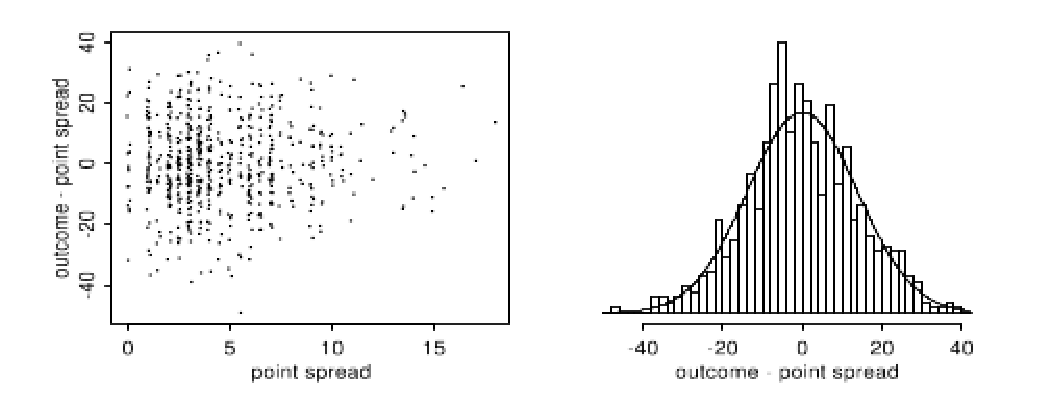
\includegraphics[scale = 0.35]{pictures/fig_1_2.eps}
\caption{Vztah mezi výskytem ischemické poruchy srdeční a věkem pacienta}
\label{fig_1_2}
\end{figure}

V následujícím textu budeme výraz $\pi(x) = E(Y | x)$ používat pro označení střední hodnoty závislé veličiny $Y$ podmíněné hodnotu $x$ pro jednorozměrný logistický regresní model, kde
\begin{equation}
\pi(x) = \frac{e^{\beta_0 + \beta_1 x}}{1 + e^{\beta_0 + \beta_1 x}}.
\end{equation}
Tuto transformaci, která je klíčová pro studium logistického regresního modelu, nazýváme logit transformací a lze ji snadno upravit do tvaru
\begin{equation}
g(x) = \ln \Big[\frac{\pi(x)}{1 - \pi(x)} \Big] = \beta_0 + \beta_1 x.
\end{equation}
Funkce $g(x)$, kterou nazýváme logit funkcí, může nabývat hodnot z intervalu $(-\infty, \infty)$.

Hodnotu závislé veličiny $y$ pro danou hodnotu $x$ můžeme vyjádřit jako $y = \pi(x) + \varepsilon$, kde $\varepsilon$ nabývá dvou stavů. Pokud $y = 1$, pak $\varepsilon = 1 -\pi(x)$ s pravděpodobností $\pi(x)$; pokud $y = 0$, pak $\varepsilon = -\pi(x)$ s pravděpodobností $1 - \pi(x)$.\footnote{Pokud $Y$ nabývá hodnot 0 popř. 1, lze $\pi(x) = E(Y | x)$ interpretovat ve smyslu pravděpodobnosti, s jakou $Y$ nabývá pro dané $x$ hodnoty 1. Pravděpodobnost, s jakou $Y$ nabývá pro dané $x$ hodnoty 0, je pak $1 - \pi(x)$.} Chyba $\varepsilon$ tak sleduje binomické rozdělení s nulovou střední hodnotou a rozptylem $\pi(x)[1 - \pi(x)]$. To je další ze zásadních rozdílů oproti lineárnímu regresnímu modelu, ve kterém chyba $\varepsilon$ sleduje normální rozdělení.

\section{Kalibrace logistického regresního modelu}

Základní metodou odhadu parametrů lineárního regresního modelu je metoda nejmenších čtverců. Podstatou této metody je volba takových hodnot parametrů $\beta_0$ a $\beta_1$, které minimalizují součet kvadrátu odchylek pozorovaných a predikovaných hodnot závislé veličiny $Y$. Tuto metodu však není v případě logistického regresního modelu možné použít.

Obecnější metodou odhadu parametrů je tzv. metoda maximální věrohodnosti, která odhadne hodnoty parametrů tak, aby výsledný model s maximální možnou pravděpodobností replikoval pozorovaná data. Za tímto účelem je třeba definovat tzv. funkci maximální věrohodnosti, která vyjadřuje pravděpodobnost výskytu pozorovaných dat v kontextu uvažovaného modelu jako funkci jeho parametrů.

Uvažujme jednorozměrný logistický regresní model a obecný pár $(x_i, y_i)$. Pokud $y_i = 1$, je kontribuce páru $(x_i, y_i)$ do funkce maximální věrohodnosti rovna $\pi(x)$. Pokud $y_i = 0$, je kontribuce páru $(x_i, y_i)$ do funkce maximální věrohodnosti rovna $1 - \pi(x)$. Tyto dva stavy lze zkombinovat do podoby
\begin{equation}
\pi(x_i)^{y_i}[1 - \pi(x_i)]^{1 - y_i}.
\end{equation}
Pokud předpokládáme, že jednotlivá pozorování představovaná páry $(x_i, y_i)$ jsou vzájemně nezávislá, lze funkci maximální věrohodnosti vyjádřit jako
\begin{equation}
l(\pmb{\beta}) = \prod_{i = 1}^n \pi(x_i)^{y_i}[1 - \pi(x_i)^{1 - y_i}].
\end{equation}
Z matematického a numerického hlediska je však snadnější pracovat s logaritmem funkce maximální věrohodnosti
\begin{equation}
L(\pmb{\beta}) = \ln[l(\pmb{\beta})] = \sum_{i = 1}^n \Big(y_i \ln[\pi(x_i) + (1 - y_i) \ln[1 - \pi(x_i)] \Big),
\end{equation}
kde $\pi(x_i) = \frac{e^{\beta_0 + \beta_1 x_i}}{1 + e^{\beta_0 + \beta_1 x_i}}$. Abychom nalezli hodnotu $\pmb{\beta}$, která maximalizuje $L(\pmb{\beta})$, je třeba nejprve derivovat $L(\pmb{\beta})$ dle $\beta_0$ a $\beta_1$ a tyto derivace položit rovny nule. Výsledné rovnice, které nazýváme rovnicemi maximální věrohodnosti, mají podobu
\begin{equation}
\sum_{i = 1}^n [y_i - \pi(x_i)] = 0
\end{equation}
a
\begin{equation}
\sum_{i = 1}^n x_i [y_i - \pi(x_i)] = 0.
\end{equation}
Rovnice maximální věrohodnosti jsou nelineární v parametrech $\beta_0$ a $\beta_1$, a proto je třeba je řešit iteračně pomocí optimalizační metody. Hodnotu $\pmb{\beta}$, která je řešením výše uvedených rovnic, značíme $\hat{\pmb{\beta}}$ a nazýváme ji odhadem maximální věrohodnosti. Podobně je $\hat{\pi}(x_i)$ odhadem maximální věrohodnosti pro $\pi(x_i)$, a platí
\begin{equation}
\hat{\pi}(x_i) = \frac{e^{\hat{\beta}_0 + \hat{\beta}_1 x_i}}{1 + e^{\hat{\beta}_0 + \hat{\beta}_1 x_i}}.
\end{equation}
Odhadnutá logit funkce pak má tvar
\begin{equation}
\hat{g}(x_i) = \hat{\beta}_0 + \hat{\beta}_1 x_i.
\end{equation}

Rovnici (1.7) lze také vyjádřit ve tvaru
\begin{equation}
\sum_{i = 1}^n y_i = \sum_{i = 1}^n \hat{\pi}(x_i),
\end{equation}
což lze interpretovat tak, že součet pozorovaných hodnot veličiny $y$ je roven součtu predikovaných hodnot.

\section{Testy významnosti odhadnutých parametrů}

\subsection{Věrohodnostní poměrový test}

Při posuzování statistické významnosti odhadnutého parametru porovnáváme pozorované hodnoty s predikovanými hodnotami získaných na základě dvou logistických regresních modelů, z nichž jeden zahrnuje zkoumanou veličinu a druhý nikoliv. Samotné porovnání modelů je pak založené na porovnání logaritmů jejich funkce maximální věrohodnosti. Pro lepší pochopení principu je užitečné o pozorovaných hodnotách přemýšlet jako o hodnotách predikovaných tzv. saturovaným model. Saturovaný logistický regresní model je takový model, který obsahuje tolik parametrů kolik je pozorovaných párů $(x_i, y_i)$.\footnote{Jednoduchým příkladem saturovaného modelu je kalibrace jednorozměrného lineárního regresního modelu na dvou pozorováních.} Porovnání pozorovaných a predikovaných hodnot je pak založeno na statistice
\begin{equation}
D = -2 \ln \Big[\frac{\textit{hodnota funkce maximální věrohodnosti kalibrovaného modelu}}{\textit{hodnota funkce maximální věrohodnosti saturovaného modelu}}\Big],
\end{equation}
kterou nazýváme věrohodnostním poměrem (likelihood ratio) a test na ní založený pak věrohodnostním poměrovým testem (likelihood ratio test). S využitím (1.6), (1.12) a skutečnosti, že pro hodnotu věrohodnostní funkce saturovaného modelu platí
\begin{equation}
l(\textit{saturovaný model}) = \prod_{i = 1}^n y_i^{y_i}(1 - y_i)^{1 - y_i},
\end{equation}
lze statistiku $D$ vyjádřit jako
\begin{equation}
D = -2 \sum_{i = 1}^n \Big[u_i \ln\Big( \frac{\hat{\pi}_i}{y_i} \Big) + (1 - y_i) \ln \Big( \frac{1 - \hat{\pi}_i}{1 - y_i} \Big) \Big],
\end{equation}
kde $\hat{\pi}_i = \hat{\pi}(x_i)$. Pokud si dále uvědomíme, že hodnota věrohodnostní funkce saturovaného modelu je vždy rovna jedné\footnote{Toto tvrzení lze snadno ověřit dosazením $y_i = 1$ a $y_i = 0$ do (1.13).}, lze (1.12) zjednodušit do podoby
\begin{equation}
D = -2 \ln (\textit{hodnota funkce maximální věrohodnosti kalibrovaného modelu}).
\end{equation}

Pro účely zhodnocení významnosti nezávislé veličiny pak porovnáváme věrohodnostní poměr $D$ pro model s a bez uvažované veličiny, tj.
\begin{multline}
G = D(\textit{hodnota funkce maximální věrohodnosti bez uvažované veličiny}) - \\
D(\textit{hodnota funkce maximální věrohodnosti s uvažovanou veličinou}),
\end{multline}
což lze dále upravit na
\begin{equation}
G = -2 \ln \left[\frac{\textit{hodnota funkce maximální věrohodnosti bez uvažované veličiny}}{\textit{hodnota funkce maximální věrohodnosti s uvažovanou veličinou}}\right].
\end{equation}
Lze snadno dokázat, že v případě modelu, který zahrnuje pouze parametr $\beta_0$, je odhad tohoto parametru roven $\ln(n_1 / n_0)$, kde $n_1 = \sum_{i = 1}^n y_i$ a $n_0 = \sum_{i = 1}^n (1 - y_i)$ a predikovaná hodnota má charakter konstanty $n_1 / n$. V tomto případě pak pro námi uvažovaný jednorozměrný logistický regresní model platí
\begin{equation}
G = -2 \ln \left[\frac{\Big(\frac{n_1}{n}\Big)^{n_1}\Big(\frac{n_0}{n}\Big)^{n_0}}{\prod_{i = 1}^n \hat{\pi}_i (1 - \hat{\pi}_i)^{1 - y_i}}\right].
\end{equation}

Při platné nulové hypotéze $H_0: \beta_1 = 0$ sleduje $G$ chi-kvadrát rozdělení s jedním stupněm volnosti.

\subsection{Waldův test}

Alternativou k věrohodnostnímu poměrovému testu je Waldův test, který poměřuje hodnotu odhadnutého parametru $\hat{\beta}_1$ k jeho směrodatné odchylce. Výsledný poměr
\begin{equation}
W = \frac{\hat{\beta}_1}{\widehat{se}(\hat{\beta}_1)}
\end{equation}
při platnosti nulové hypotézy $H_0: \beta_1 = 0$ sleduje standardní normální rozdělení. Nevýhodou Waldova testu bohužel je, že často nezamítne nulovou hypotézu ani v případě, kdy je odhadnutý parametr významný. Proto je vhodnější používat věrohodnostní poměrový test.

\subsection{Skóre test}

Dalším možným testem významnosti parametru je tzv. skóre test, jehož hlavní výhodou je nižší výpočetní náročnost. Test je založen na teorii pravděpodobnostního rozdělení derivace logaritmu věrohodnostní funkce. Konkrétně v případě jednorozměrného logistického regresního modelu je test založen na znalosti pravděpodobnostního rozdělení derivace (1.8) podmíněné derivací (1.7). Test používá hodnotu rovnice (1.8) vypočtenou s pomocí $\beta_0 = \ln(n_1 / n_0)$ a $\beta_1 = 0$. Jak již bylo zmíněno dříve, platí pro tento případ $\hat{\pi} = n_1 / n = \overline{y}$. Dále lze dokázat, že odhadovaný rozptyl je $\overline{y}(1 - \overline{y}) \sum (x_i - \overline{x})^2$. To vede ke statistice
\begin{equation}
ST = \frac{\sum_{i = 1}^n x_i (y_i - \overline{y})}{\sqrt{\overline{y}(1 - \overline{y}) \sum_{i = 1}^n (x_i - \overline{x})^2}},
\end{equation}
která opět sleduje standardizované normální rozdělení. Opět nicméně platí, že věrohodnostní poměrový test je preferovaný před skóre testem.

\section{Intervaly spolehlivosti}

Intervaly spolehlivosti odhadnutých parametrů jsou založeny na Waldově testu a mají tvar
\begin{equation}
\hat{\beta}_i \pm z_{1 - \alpha / 2} \widehat{se}(\hat{\beta}_i).
\end{equation}
Takto definované intervaly spolehlivosti lze použít nejen pro $\beta_1$ ale také pro konstantní člen modelu $\beta_0$.

Podobným způsobem lze také odhadnout intervaly spolehlivosti pro logit funkci. Střední hodnota logit funkce je definována jako
\begin{equation}
\hat{g}(x) = \hat{\beta}_0 + \hat{\beta}_1 x
\end{equation}
a její rozptyl v případě jednorozměrného logistického regresního modelu jako
\begin{equation}
\widehat{var}[g(x)] = \widehat{var}(\hat{\beta}_0) + x^2 \widehat{var}(\hat{\beta}_1) + 2 x \widehat{cov}(\hat{\beta}_0, \hat{\beta}_1).
\end{equation}
Interval spolehlivosti logit funkce pak lze vypočíst pomocí
\begin{equation}
\hat{g}(x) \pm z_{1 - \alpha / 2}\widehat{se}[\hat{g}(x)],
\end{equation}
kde $\widehat{se}[\hat{g}(x)] = \sqrt{\widehat{var}[g(x)]}$. Protože střední hodnota $\hat{\pi}(x)$ je definována jako $\frac{e^{\hat{g}(x)}}{1 + e^{\hat{g}(x)}}$, lze interval spolehlivosti pro $\hat{\pi}(x)$ určit pomocí
\begin{equation}
\frac{e^{\hat{g}(x) \pm z_{1 - \alpha / 2} \widehat{se}[\hat{g}(x)]}}{1 + e^{\hat{g}(x) \pm z_{1 - \alpha / 2} \widehat{se}[\hat{g}(x)]}}.
\end{equation}

\chapter{Vícerozměrný logistický regresní model}

\section{Vícerozměrný logistický regresní model}

Logit funkce vícerozměrného logistického regresního modelu má podobu
\begin{equation}
g(\pmb{x}) = \beta_0 + \beta_1 x_1 + \beta_2 x_2 + ... + \beta_p x_p
\end{equation}
a samotný logistický regresní model pak podobu
\begin{equation}
\pi(\pmb{x}) = \frac{e^{g(\pmb{x})}}{1 + e^{g(\pmb{x})}}.
\end{equation}

Pokud je některá z nezávislých veličin diskrétní numerická veličina, jejíž hodnoty označují jednotlivé kategorie (např. rasu nebo pohlaví), nelze s nimi nakládat jako s klasickými numerickými veličinami. V následujícím textu budeme tyto veličiny označovat jako kategorické. V případě numerické veličiny představují její hodnoty rozdílné úrovně; v případě kategorických veličin představují jejich hodnoty jednotlivé kategorie, které nemají ordinální význam. Pokud nabývá kategorická veličina $k$ různých hodnot, je třeba ji nahradit $k-1$ pomocnými binárními proměnnými. Pokud např. nezávislá veličina $X_i$ představující rasu nabývá hodnot 0 pro bělocha, 1 pro černocha a 2 pro asiata, je třeba ji nahradit pomocnými nezávislými veličinami $D_{i1}$, která nabývá hodnoty 1 pro černocha a 0 pro ostatní rasy, a $D_{i2}$, která nabývá hodnoty 1 pro asiata a hodnoty nula pro ostatní rasy. Je třeba zdůraznit, že není možné do modelu zahrnout také pomocnou proměnnou $D_{i3}$, která by nabývala hodnoty 1 pro bělocha, protože bychom tímto vytvořili perfektní multikolinearitu. Vícerozměrná logit funkce s kategorickou veličinou $X_j$, která nabývá $k_j$ hodnot tak má podobu
\begin{equation}
g(\pmb{x}) = \beta_0 + \beta_1 x_1 + ... + \sum_{l = 1}^{k_j - 1} \beta_{jl}D_{jl} + \beta_p x_p.
\end{equation}

\section{Kalibrace vícerozměrného logistického regresního modelu}

Stejně jako v případě jednorozměrného logistického regresního modelu také v případě vícerozměrného logistického regresního modelu se pro jeho kalibraci používá metody maximální věrohodnosti.

Uvažujme model definovaný logit funkcí (2.1). Derivací logaritmu odpovídající věrohodnostní funkce podle $p + 1$ parametrů získáme jednu rovnici maximální věrohodnosti ve tvaru
\begin{equation}
\sum_{i = 1}^n [y_i - \pi(\pmb{x}_i)] = 0
\end{equation}
a $p$ rovnic maximální věrohodnosti ve tvaru
\begin{equation}
\sum_{i = 1}^n x_{ij} [y_i - \pi(\pmb{x}_i)] = 0.
\end{equation}
Tyto rovnice lze použít pro odhad hodnot parametrů jednotlivých veličin pomocí optimalizační metody.

Kromě bodového odhadu parametrů je třeba také získat odhad jejich směrodatných odchylek. Příslušné odhady lze vypočíst ze soustavy rovnic druhých parciálních derivací logaritmu věrohodnostní funkce, které mají podobu
\begin{equation}
\frac{\partial^2 L(\pmb{\beta)}}{\partial \beta_j^2} = - \sum_{i = 1}^n x_{ij}^2 \pi_i(1 - \pi_i)
\end{equation}
a
\begin{equation}
\frac{\partial^2 L(\pmb{\beta})}{\partial \beta_j \partial \beta_l} = - \sum_{i = 1}^n x_{ij} x_{il} \pi_i (1 - \pi_i),
\end{equation}
pro $j, l = 0, 1, ..., p$, kde $\pi_i$ označuje $\pi(\pmb{x}_i)$. Matici $(p + 1) \times (p + 1)$ sestávající se ze záporných členů daných rovnicemi (2.6) a (2.7) označme jako $\pmb{I}(\pmb{\beta})$. Tato matice se nazývá pozorovaná informační matice (observed information matrix). Rozptyl a kovariance jednotlivých parametrů lze získat z inverze této matice, kterou budeme označovat jako $var(\pmb{\beta}) = \pmb{I}^{-1}(\pmb{\beta})$. Bohužel až na výjimečné případy není možné explicitně vyjádřit členy matice $var(\pmb{\beta})$. V následujícím textu budeme používat $var(\beta_j)$ k označení $j$-tého členu diagonály této matice, který představuje rozptyl odhadu $\hat{\beta}_j$, a $cov(\beta_j, \beta_l)$ k označení členů mimo diagonálu, které představují kovarianci mezi odhady $\hat{\beta}_j$ a $\hat{\beta}_l$. Jejich odhady jsou pak získány vyhodnocením matice $var(\pmb{\beta})$ pro $\hat{\pmb{\beta}}$.

Odhad informační matice lze vyjádřit ve tvaru $\hat{\pmb{I}}(\hat{\pmb{\beta}}) = X'VX$, kde
\begin{equation}
X =
\begin{bmatrix}
1 & x_{11} & x_{12} & \cdots & x_{1p}\\
1 & x_{21} & x_{22} & \cdots & x_{2p}\\
\vdots & \vdots & \vdots & \cdots & \vdots\\
1 & x_{n1} & x_{n2} & \cdots & x_{np}
\end{bmatrix}
\end{equation}
a
\begin{equation}
V =
\begin{bmatrix}
\hat{\pi}_1 (1 - \hat{\pi}_1) & 0 & \cdots & 0\\
0 & \hat{\pi}_2(1 - \hat{\pi}_2) & \cdots & 0\\
\vdots & 0 & \ddots & \vdots\\
0 & \cdots & 0 & \hat{\pi}_n (1 - \hat{\pi}_n) 
\end{bmatrix}.
\end{equation}

\section{Testy významnosti odhadnutých parametrů}

\subsection{Věrohodnostní poměrový test}

Stejně jako v případě jednorozměrného logistického regresního modelu lze také v případě vícerozměrného logistického regresního modelu použít pro posouzení významnosti odhadnutých parametrů věrohodnostní poměrový test.

Uvažujme vícerozměrný logistický model s $p$ nezávislými veličinami. Pro nulovou hypotézu předpokládáme, že hodnoty všech $p$ odhadnutých parametrů jsou rovny nule a že distribuce odpovídající $G$ statistiky sleduje chi-kvadrát rozdělení $p$ stupni volnosti. Pro úplnost připomeňme, že $G$ je podílem logaritmu věrohodnostní funkce modelu obsahujícího všech $p$ veličin a modelu obsahujícího pouze konstantní člen.

Analogickou formu věrohodnostního poměrového testu lze použít také k testování menšího počet odhadnutých parametrů a to včetně testování významnosti jednoho parametru. Jediným rozdílem je, že se při výpočtu statistiky $G$ namísto modelu obsahujícího pouze konstantní člen použije příslušný redukovaný model a odpovídajícím způsobem se upraví počet stupňů volnosti.

\subsection{Waldův test}

\subsubsection{Jednorozměrný Waldův test}

Při testování statistické významnosti jednoho odhadnutého parametru lze použít také Waldův test, jehož statistika má podobu
\begin{equation}
W_j = \frac{\hat{\beta}_j}{\widehat{se}(\hat{\beta}_j)},
\end{equation}
a která sleduje standardní normální rozdělení.

Jak již bylo zmíněno výše, pokud nezávislá proměnná nabývá $k > 2$ kategorií, je třeba ji ``přeformulovat" pomocných $k - 1$ binárních veličin. Jestliže na tyto pomocné binární veličiny aplikujeme Waldův test, může jedna veličina vyjít jako statisticky významná, zatímco ostatní veličiny jako statisticky nevýznamné. V tomto případě je žádoucí v modelu buď ponechat všechny nebo naopak žádnou z těchto pomocných veličin. Toto pravidlo se vztahuje také na ostatní typy testů statistické významnosti.

\subsubsection{Vícerozměrný Waldův test}

Kromě výše popsaného Waldova testu významnosti existuje také jeho vícerozměrná varianta. Jeho statistika je pak vypočtena jako
\begin{equation}
W = \hat{\pmb{\beta}}' \left[\widehat{var}(\hat{\pmb{\beta}})\right]^{-1} \hat{\pmb{\beta}} = \hat{\pmb{\beta}}' (\pmb{X}' V \pmb{X}) \hat{\pmb{\beta}}
\end{equation}
a sleduje chi-kvadrát rozdělení s $p$ stupni volnosti při hypotéze, že $p$ odhadnutých parametrů je rovno nule. Testy pro méně než $p$ parametrů jsou definovány analogicky.

Vyhodnocení vícerozměrného Waldova testu vyžaduje poměrně velkou výpočetní kapacitu, nenabízí tato metoda žádnou zásadnější výhodu oproti věrohodnostnímu poměrovému testu.

\subsection{Skóre test}

Vícerozměrná varianta skóre testu je založena na rozdělení $p$ derivací $L(\pmb{\beta})$ vzhledem k $\pmb{\beta}$. Nicméně podobně jako v případě Waldova testu i vícerozměrná varianta skóre testu je poměrně výpočetně náročná, a proto se upřednostňuje věrohodnostní poměrový test.

\section{Intervaly spolehlivosti}

Intervaly spolehlivosti jednotlivých parametrů jsou konstruovány stejným způsobem jako v případě jednorozměrného logistického regresního modelu, tj.
\begin{equation}
\hat{\beta}_i \pm z_{1 - \alpha / 2}\widehat{se}(\hat{\beta}_i).
\end{equation}
Podobně lze určit též interval spolehlivosti logit funkce jako
\begin{equation}
\hat{g}(\pmb{x}) \pm z_{1 - \alpha / 2}\widehat{se}(\hat{g}(\pmb{x})),
\end{equation}
kde
\begin{equation}
\hat{g}(\pmb{x}) = \hat{\beta}_0 + \hat{\beta}_1 x_1 + \hat{\beta}_2 x_2 + ... + \hat{\beta}_p x_p
\end{equation}
a
\begin{equation}
\widehat{se}[\hat{g}(\pmb{x})] = \sqrt{\widehat{var}[\hat{g}(\pmb{x})]} = \sqrt{\sum_{j = 0}^p x^2_j \widehat{var}(\hat{\beta}_j) + \sum_{j = 0}^p \sum_{k = j + 1}^p 2 x_j x_k \widehat{cov}(\hat{\beta}_j, \hat{\beta}_k)}.
\end{equation}
Maticově lze $\widehat{var}[\hat{g}(\pmb{x})]$ vyjádřit také jako
\begin{equation}
\widehat{var}[\hat{g}(\pmb{x})] = \pmb{x}' \widehat{var}(\hat{\pmb{\beta}}) \pmb{x} = \pmb{x}' (\pmb{X'VX})^{-1} \pmb{x}.
\end{equation}
\chapter{Interpretace logistického regresního modelu}

\section{Úvod}

Předpokladem interpretace libovolného nakalibrovaného modelu je, že jsme schopni smysluplně interpretovat jeho odhadnuté parametry. Tato interpretace zahrnuje dva kroky - (a) odhad funkcionálního vztahu mezi závislou a nezávislou veličinou a (b) definování vhodné jednotky změny nezávislé veličiny.

První krok předpokládá, že vztah mezi závislou a nezávislou veličinou lze popsat pomocí lineární funkce. V případě jednorozměrného lineárního regresního modelu má tento vztah podobu $y(x) = \beta_0 + \beta_1 x$. V případě logistického regresního modelu je tento vztah definován na úrovni logit funkce, tj. jako $g(x) = \ln \left(\frac{\pi(x)}{1 - \pi(x)}\right) = \beta_0 + \beta_1 x$.

Co se druhého kroku týče, je v případě jednorozměrného lineárního regresního modelu koeficient $\beta_1$ definován jako změna hodnoty závislé veličiny pro jednotkovou změnu závislé veličiny, tj. $\beta_1 = y(x + 1) - y(x)$. Naproti tomu v případě logistického regresního modelu představuje koeficient $\beta_1$ změnu v logit funkci, tj. $\beta_1 = g(x + 1) - g(x)$.

\section{Nezávislá binární veličina}

Nezávislou veličinu nazýváme binární, pokud nabývá pouze dvou hodnot. V následujícím textu budeme předpokládat, že taková veličina nabývá hodnot 0 a 1. Změna v logit funkci tak má podobu
\begin{equation}
g(1) - g(0) = [\beta_0 + \beta_1] - [\beta_0] = \beta_1.
\end{equation}
Možné kombinace logistické pravděpodobnosti jsou ilustrovány tabulkou na obrázku (3.1).
\begin{figure}[htp]
\centering
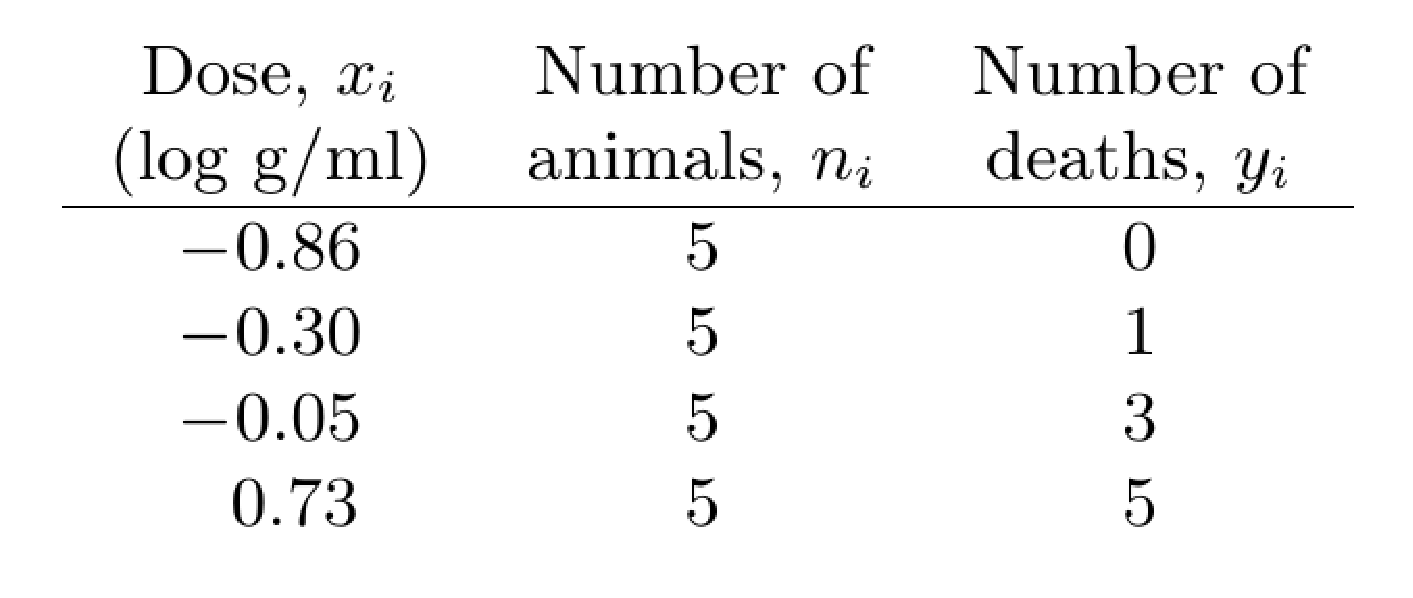
\includegraphics[scale = 0.35]{pictures/tbl_3_1.eps}
\caption{Hodnoty jednorozměrného logistického regresního modelu pro binární nezávislou veličinu}
\label{tbl_3_1}
\end{figure}

Důležitou statistikou používanou při analýze logistického regresního modelu je tzv. podíl rizik (odd ratio), které je definovaný jako
\begin{equation}
OR = \frac{\pi(1) / [1 - \pi(1)]}{\pi(0) / [1 - \pi(0)]}.
\end{equation}
V případě jednorozměrné logistické regrese s binární nezávislou veličinou, která nabývá hodnot 0 nebo 1, je vztah mezi podílem rizik a hodnotou regresního parametru definován jako
\begin{equation}
OR = \frac{\pi(1) / [1 - \pi(1)]}{\pi(0) / [1 - \pi(0)]} = \frac{\frac{e^{\beta_0 + \beta_1}}{1 + e^{\beta_0 + \beta_1}} \Big/ \frac{1}{1 + e^{\beta_0 + \beta_1}}}{\frac{e^{\beta_0}}{1 + e^{\beta_0}} \Big/ \frac{1}{1 + e^{\beta_0}}} = \frac{e^{\beta_0 + \beta_1}}{e^{\beta_0}} = e^{(\beta_0 + \beta_1) - \beta_0} = e^{\beta_1}.
\end{equation}
Podíl rizik přibližně vyjadřuje kolikrát je pravděpodobnější výskyt pozitivní hodnoty závislé veličiny pro pozorování $x = 1$ než pro pozorování $x = 0$. Pokud např. $y$ označuje výskyt / absenci rakoviny plic $x$ obsahuje informaci o tom, zda-li je daná osoba kuřák, pak $\widehat{OR} = 2$ znamená, že pravděpodobnost výskytu rakoviny plic u kuřáka je dvakrát vyšší než u nekuřáka. Vzhledem k definici podílu rizik je zřejmé, že tato statistika přibližně vyjadřuje tzv. relativní riziko, které je definováno jako $\pi(1) / \pi(0)$. Z tabulky (3.1) je pak zřejmé, že tato aproximace platí, pokud $[1 - \pi(0)] / [1 - \pi(1)] \approx 1$. To je splněno, pokud $\pi(x)$ je malé jak pro $x = 1$ tak pro $x = 0$.

V řadě aplikací logistické regrese, se kterými se můžeme setkat v odborné literatuře, jsou spojité numerické veličiny převedeny na binární pomocí vhodně zvoleného hraničního bodu. Pro ilustraci uvádíme klasifikační tabulku (3.2), kdy veličina $AGED$ nabývá hodnoty 0 pokud je dané osobě méně než 55 let a hodnoty 1 v ostatních případech.
\begin{figure}[htp]
\centering
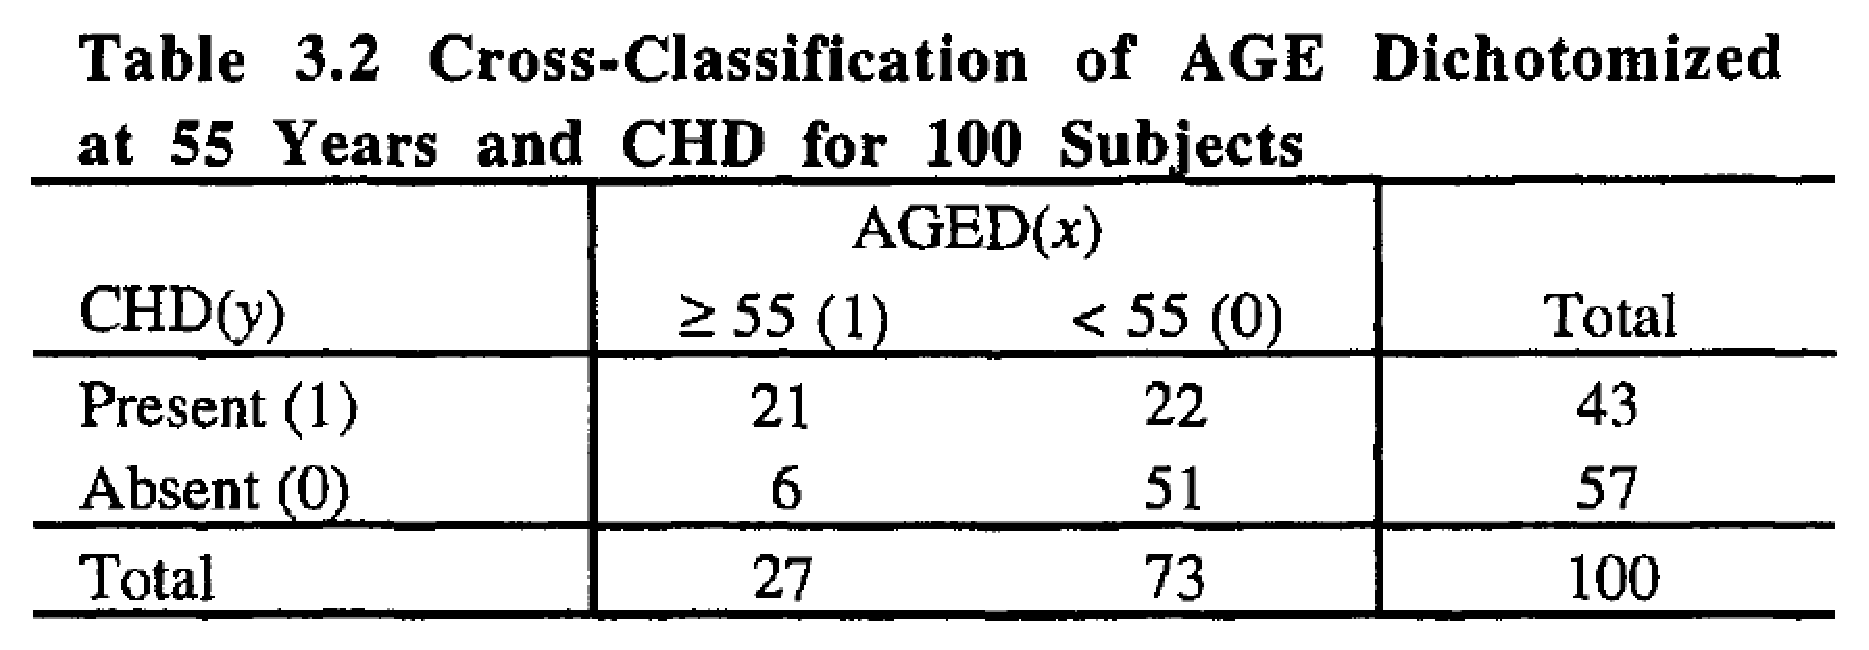
\includegraphics[scale = 0.35]{pictures/tbl_3_2.eps}
\caption{Klasifikační tabulka pro binární nezávislou veličinu $AGED$ a závislou veličinu $CHD$ představující výskyt ischemické choroby srdeční.}
\label{tbl_3_2}
\end{figure}
Zkoumaná populace se dle tabulky (3.2) skládala z 21 osob s hodnotami $(x = 1, y = 1)$, 22 osob s hodnotami $(x = 0, y = 1)$, 6 osob s hodnotami $(x = 1, y = 0)$ a 51 osob s hodnotami $x = 0, y = 0$. Pokud bychom na základě těchto dat odhadli metodou maximální věrohodnosti parametr pro veličinu $AGED$, získali bychom hodnotu 2.094. Podíl rizik bychom pak odhadli na $\widehat{OR} = e^{2.094} = 8.1$. Podíl rizik však lze odhadnout také přímo s pomocí klasifikační tabulky, tj. jako
\begin{equation}
\widehat{OR} = \frac{\hat{\pi}(1) / [1 - \hat{\pi}(1)]}{\hat{\pi}(0) / [1 - \hat{\pi}(0)]} = \frac{21/6}{22/51} = 8.11.
\end{equation}
Interval spolehlivosti podílu rizik se pak určí tak, že se nejprve vypočtou krajní hodnoty odpovídající intervalu spolehlivosti odhadu parametru $\beta_1$ a na ně se aplikuje exponenciála, tj.
\begin{equation}
e^{\beta_1 \pm z_{1 - \alpha / 2} \widehat{se}(\hat{\beta}_1)}.
\end{equation}
Vzhledem ke způsobu konstrukce je interval spolehlivosti podílu rizik nesymetrický.

V předchozím textu jsme předpokládali, že nezávislá binární veličina $x$ nabývá veličin 0 a 1. Je třeba zdůraznit, že výše uvedené závěry jsou platné pouze pro tento případě. Uvažujme situaci, kdy $x$ nabývá dvou různých obecných hodnot $a$ a $b$. Pak platí
\begin{equation}
\ln[\widehat{OR}(a, b)] = \hat{g}(x = a) - \hat{g}(x = b) = (\hat{\beta}_0 + \hat{\beta}_1 a) - (\hat{\beta}_0 + \hat{\beta}_1 b) = \hat{\beta}_1 (a - b)
\end{equation}
neboli
\begin{equation}
\widehat{a, b} = e^{\hat{\beta}_1 (a - b)}.
\end{equation}
Analogie (3.2) pak má podobu
\begin{equation}
\widehat{OR}(a, b) = \frac{\hat{\pi}(x = a) / [1 - \hat{\pi}(x = a)]}{\hat{\pi}(x = b) / [1 - \hat{\pi}(x = b)]}.
\end{equation}
Interval spolehlivosti podílu rizik lze vyjádřit jako
\begin{equation}
e^{\hat{\beta}_1(a - b) \pm z_{1 - \alpha / 2}|a - b| \widehat{se}(\hat{\beta}_1)}.
\end{equation}
Je třeba zdůraznit, že kódování binární proměnné do 0 a 1 je zdaleka nejčastější, a proto ho budeme používat i v následujícím textu. Dalším používaným kódováním je pak -1 a 1, které je však méně frekventované.

\section{Nezávislá kategorická veličina}

Kategorickou veličinou rozumíme veličinu, která může nabývat $k > 2$ různých nominální hodnot. Jak jsme již zmínili výše, takovouto veličinu musíme převést na $k - 1$ pomocných binárních veličin. Jako příklad uveďme veličinu $X_i$, která nabývá hodnot 0 pro bělocha, 1 pro černocha a 2 pro asiata. Tuto veličinu musíme nahradit dvojicí pomocných binárních veličin $D_{i1}$ a $D_{i2}$. Při nejčastěji používaném kódování nabývá veličina $D_{i1}$ hodnoty 1, pokud je daná osoba černoch, a 0 v ostatních případech. Podobně veličina $D_{i2}$ nabývá hodnoty 1, pokud je daná osoba asiat, a 0 v ostatních případech. Je třeba zdůraznit, že pokud bych do modelu přidali ještě třetí veličinu, $D_{i3}$, která by nabývala hodnoty 1, pokud je daná osoba běloch, a 0 v ostatních případech, vytvořili bychom perfektní multikolinearitu.\footnote{Informaci o tom, že je daná osoba běloch totiž, lze získat také na základě veličin $D_{i1}$ a $D_{i2}$. Konkrétně, pokud obě veličiny nabývají hodnoty 0, víme, že se nejedná ani o černocha a ani o asiata, takže se musí jednat o bělocha. Informace představovaná veličinou $D_{i3}$ je tak duplicitní.}

Pro ilustraci uvažujme model $y(\pmb{x}) = \beta_0 + \beta_1 D_{i1} + \beta_2 D_{i2}$, kde $y = 1$ představuje výskyt ischemické choroby srdeční. Pokud použijeme standardní kódování pomocných binárních veličin na hodnoty 0 a 1, platí
\begin{equation}
\ln[\widehat{OR}(\textit{black}, \textit{white})] = \hat{g}(\textit{black}) - \hat{g}(\textit{white}) = (\hat{\beta}_0 + \hat{\beta}_1 \cdot 1 + \hat{\beta}_2 \cdot 0) - (\hat{\beta}_0 + \hat{\beta}_1 \cdot 0 + \hat{\beta}_2 \cdot 0) = \hat{\beta}_1.
\end{equation}
Jak vyplývá z označení $\widehat{OR}(\textit{black}, \textit{white})$, vyjadřuje $\hat{\beta}_1$ odhad, kolikrát je výskyt ischemické choroby srdeční pravděpodobnější u černocha než u bělocha.  Pokud bychom chtěli porovnat pravděpodobnosti výskytu ischemické choroby srdeční pro černocha vs. asiata, museli bychom výše uvedenou rovnici upravit do tvaru
\begin{multline}
\ln[\widehat{OR}(\textit{black}, \textit{asian})] = \hat{g}(\textit{black}) - \hat{g}(\textit{asian}) =\\(\hat{\beta}_0 + \hat{\beta}_1 \cdot 1 + \hat{\beta}_2 \cdot 0) - (\hat{\beta}_0 + \hat{\beta}_1 \cdot 0 + \hat{\beta}_2 \cdot 1) = \hat{\beta}_1 - \hat{\beta}_2.
\end{multline}
Interval spolehlivosti $\widehat{OR}(\textit{black}, \textit{white})$ pak má podobu
\begin{equation}
e^{\hat{\beta}_1 \pm z_{1 - \alpha / 2} \sqrt{\widehat{var}\big(\ln[\widehat{OR}(\textit{black}, \textit{white})]\big)}} = e^{\hat{\beta}_1 \pm z_{1 - \alpha / 2} \widehat{se}(\hat{\beta}_1)}
\end{equation}
a interval spolehlivosti $\widehat{OR}(\textit{black}, \textit{asian})$ podobu
\begin{equation}
e^{(\hat{\beta}_1 - \hat{\beta}_2) \pm z_{1 - \alpha / 2} \sqrt{\widehat{var}\big(\ln[\widehat{OR}(\textit{black}, \textit{asian})]\big)}},
\end{equation}
kde
\begin{equation}
\widehat{var}\big(\ln[\widehat{OR}(\textit{black}, \textit{asian})]\big) = \widehat{var}(\hat{\beta}_1) - 2 \hat{\beta}_1 \hat{\beta}_2 \widehat{cov}(\hat{\beta}_1, \hat{\beta}_2) + \widehat{var}(\hat{\beta}_2).
\end{equation}

Dalším možným způsobem kódování je použití hodnot -1, 0 a 1. Běloch je tak reprezentován hodnotami -1 pro $D_{i1}$ a -1 pro $D_i2$, černoch hodnotami 1 pro $D_{i1}$ a 0 pro $D_{i2}$ a konečně asiat hodnotami 0 pro $D_{i1}$ a 1 pro $D_{i2}$. Platí tedy
\begin{equation}
\ln[\widehat{OR}(\textit{black}, \textit{white})] = \hat{g}(\textit{black}) - \hat{g}(\textit{white}) = (\hat{\beta}_0 + \hat{\beta}_1 \cdot 1 + \hat{\beta}_2 \cdot 0) - (\hat{\beta}_0 + \hat{\beta}_1 \cdot (-1) + \hat{\beta}_2 \cdot (-1)) = 2\hat{\beta}_1 + \hat{\beta}_2
\end{equation}
a podobně
\begin{equation}
\ln[\widehat{OR}(\textit{black}, \textit{asian})] = \hat{g}(\textit{black}) - \hat{g}(\textit{asian}) = (\hat{\beta}_0 + \hat{\beta}_1 \cdot 1 + \hat{\beta}_2 \cdot 0) - (\hat{\beta}_0 + \hat{\beta}_1 \cdot 0 + \hat{\beta}_2 \cdot 1) = \hat{\beta}_1 - \hat{\beta}_2
\end{equation}.
Intervaly spolehlivosti podílů rizik pak mají podobu
\begin{equation}
e^{(2\hat{\beta}_1 + \hat{\beta}_2) \pm z_{1 - \alpha / 2} \sqrt{\widehat{var}\big(\ln[\widehat{OR}(\textit{black}, \textit{white})]\big)}}
\end{equation}
pro $\widehat{OR}(\textit{black}, \textit{white})$ a
\begin{equation}
e^{(\hat{\beta}_1 - \hat{\beta}_2) \pm z_{1 - \alpha / 2} \sqrt{\widehat{var}\big(\ln[\widehat{OR}(\textit{black}, \textit{asian})]\big)}}
\end{equation}
pro $\widehat{OR}(\textit{black}, \textit{asian})$ kde
\begin{equation}
\widehat{var}\big(\ln[\widehat{OR}(\textit{black}, \textit{white})]\big) = 4\widehat{var}(\hat{\beta}_1) + 4 \hat{\beta}_1 \hat{\beta}_2 \widehat{cov}(\hat{\beta}_1, \hat{\beta}_2) + \widehat{var}(\hat{\beta}_2).
\end{equation}
a
\begin{equation}
\widehat{var}\big(\ln[\widehat{OR}(\textit{black}, \textit{asian})]\big) = \widehat{var}(\hat{\beta}_1) - 2 \hat{\beta}_1 \hat{\beta}_2 \widehat{cov}(\hat{\beta}_1, \hat{\beta}_2) + \widehat{var}(\hat{\beta}_2).
\end{equation}
Tento způsob kódování je však používán spíše výjimečně, a proto budeme v následujícím textu používat kódování pomocí hodnot 0 a 1.
\chapter{Asymptotické vlastnosti a souvislost s nebayesiánskými\\ metodami}

\section{Normální aproximace aposteriorního rozdělení}

\subsection{Normální aproximace aposteriorního sdruženého rozdělení}

Jestliže je aposteriorní rozdělení $p(\theta|y)$ unimodální a přibližně symetrické, můžeme ho aproximovat pomocí normální rozdělení, tj. logaritmus aposteriorního rozdělení aproximujeme kvadratickou funkcí parametru $\theta$.

Taylorovým rozvojem $\ln(p(y|\theta))$ centrovaným na aposteriorní mód $\hat{\theta}$ získáváme
\begin{equation}
\ln\big(p(\theta|y)\big) = \ln\big(p(\hat{\theta}|y)\big) + \frac{1}{2}(\theta - \hat{\theta})^T \Big[\frac{d^2}{d \theta^2}\ln\big(p(\theta|y)\big)\Big]_{\theta = \hat{\theta}}(\theta - \hat{\theta}) + ...,
\end{equation}
kde lineární člen rozvoje je nulový, protože derivace pravděpodobnostního rozdělení v jeho módu je rovna nule. Vyšší členy rozvoje můžeme vzhledem k jejich kvadratické formě zanedbat, pokud je $\theta$ dostatečně blízko $\hat{\theta}$ a $n$ dostatečně velké.

První člen rozvoje (4.1) je konstantní a druhý člen je proporcionální logaritmu normálního rozdělení, což vede k aproximaci
\begin{equation}
p(\theta | y) \approx N(\hat{\theta}, [I(\hat{\theta})]^{-1}),
\end{equation}
kde $I(\theta)$ je
\begin{equation}
I(\theta) = - \frac{d^2}{d \theta^2} \ln(p(\theta|y)).
\end{equation}
Jestliže se mód aposteriorního rozdělení $\hat{\theta}$ nachází uvnitř parametrového prostoru, pak je matice $I(\hat{\theta})$ pozitivně definitní.

\subsubsection{Ilustrativní příklad - normální rozdělení s neznámou střední hodnotou a rozptylem}

Nechť $(y_1,..., y_n)$ jsou nezávislá pozorování z $N(\mu, \sigma^2)$ a předpokládejme apriorní uniformní rozdělení pro parametry $(\mu, \ln(\sigma))$. Abychom mohli zkonstruovat výše uvedenou aproximaci, potřebujeme druhou derivaci logaritmu aposteriorního rozdělení,
\begin{equation}
\ln\big(p(\mu, \ln(\sigma)|y)\big) = \textit{konstanta} - n \ln(\sigma) - \frac{1}{2 \sigma^2}\big((n - 1)s^2 + n(\overline{y} - \mu)\big).
\end{equation}
První derivace mají podobu
\begin{equation}
\frac{d}{d \mu} \ln\big(p(\mu, \ln(\sigma)|y)\big) = \frac{n(\overline{y} - \mu)}{\sigma^2},
\end{equation}
\begin{equation}
\frac{d}{d\big(\ln(\sigma)\big)} \ln\big(p(\mu, \ln(\sigma)|y)\big) = -n + \frac{(n - 1)s^2 + n(\overline{y} - \mu)^2}{\sigma^2},
\end{equation}
z nichž lze s pomocí vztahů $\frac{d}{d \mu} = 0$ a $\frac{d}{d(\ln(\sigma))} = 0$ vypočíst mód
\begin{equation}
\big(\hat{\mu}, \ln(\hat{\sigma})\big) = \Big(\overline{y}, \ln\Big(\sqrt{\frac{n - 1}{n}}s\Big)\Big).
\end{equation}
Druhé derivace logaritmu aposteriorního rozdělení jsou pak
\begin{equation}
\frac{d^2}{d \mu^2} \ln\big(p(\mu, \ln(\sigma)|y)\big) = - \frac{n}{\sigma^2},
\end{equation}
\begin{equation}
\frac{d^2}{d \mu d\big(\ln(\sigma)\big)} \ln\big(\mu, \ln(\sigma)|y\big) = -2n \frac{\overline{y} - \mu}{\sigma^2},
\end{equation}
\begin{equation}
\frac{d^2}{d\big(\ln(\sigma)\big)^2}\ln\big(p(\mu, \ln(\sigma)|y)\big) = -\frac{2}{\sigma^2}\big((n - 1)s^2 + n(\overline{y} - \mu)^2 \big).
\end{equation}
Matice druhých derivací v módu je tak
\begin{equation}
\begin{bmatrix}
-n / \hat{\sigma}^2 & 0\\
0 & -2n\\
\end{bmatrix}.
\end{equation}
Pomocí (4.2) tak lze aposteriorní rozdělení aproximovat jako
\begin{equation}
p\big(\mu, \ln(\sigma)|y \big) \approx N \Big(\begin{bmatrix}\mu \\ \ln(\sigma) \end{bmatrix} \Bigm| \begin{bmatrix}\overline{y} \\ \ln(\hat{\sigma}) \end{bmatrix},  \begin{bmatrix}\hat{\sigma}^2 / n & 0\\ 0 & 1 / (2n) \end{bmatrix}\Big).
\end{equation}

Pokud bychom aproximaci konstruovali s pomocí $p(\mu, \sigma^2)$ namísto $p\big(\mu, \ln(\sigma)\big)$, pak bychom matici obsahující derivace druhého řádu násobili Jakobiánem transformační matice z $\ln(\sigma)$ na $\sigma^2$. To by vedlo je změně módu na $\hat{\sigma}^2 = \frac{n}{n + 2}\hat{\sigma}^2$. Obě komponenty parametru $(\mu, \sigma^2)$ by byly rámci aproximace aposteriorního rozdělení stále nezávislé a platilo by $p(\sigma^2 | y) \approx N\big(\sigma^2| \tilde{\sigma}^2, 2 \tilde{\sigma}^4 / (n + 2)\big)$.

\subsection{Interpretace aposteriorního rozdělení s ohledem na jeho maximum}

Kromě aproximace lze vícerozměrné normální rozdělení použít také při interpretaci konturových grafů (contour plots). V případě $d$-rozměrného normálního rozdělení je totiž logaritmus jeho hustoty pravděpodobnosti roven součtu konstanty a $\chi_d^2$ rozdělení vyděleného členem $-2$. Např. 95\% kvantil $\chi_{10}^2$ rozdělení je roven 18.31. Pokud má tedy námi řešený problém $d = 10$ parametrů, pak je 95\% aposteriorní pravděpodobnostní masy spojeno s hodnotami parametru $\theta$, pro které je $p(\theta|y)$ alespoň $e^{-18.31 / 2} = 1.1 \cdot 10^{-4}$ krát pravděpodobnostní hustota v módu. Podobně pro $d = 2$ parametrů odpovídá 95\% aposteriorní pravděpodobnostní masy přibližně hustotě $e^{-5.99 / 2} = 0.05$ a více relativně vzhledem k módu.

\subsection{Předpoklad normality}

Pokud je $n$ dostatečně veliké, často se implicitně předpokládá, že aposteriorní rozdělení může být aproximováno pomocí normálního rozdělení. V praxi je však poměrně obtížné ověřit míru splnění tohoto předpokladu. V řadě případů lze konvergenci k normálnímu rozdělení zlepšit pomocí transformace. Pokud je $\phi$ spojitá transformace parametru $\theta$, pak se jak $p(\phi | y)$ tak $p(\theta | y)$ blíží normálnímu rozdělení, nicméně míra přiblížení se normálnímu rozdělení se v může výrazně lišit podle zvolené transformace.

\subsection{Redukce dat a souhrnné statistiky}

Při aproximaci pomocí normálního rozdělení lze aposteriorní rozdělení souhrnně popsat pomocí módu $\hat{\theta}$ a zakřivení aposteriorního rozdělení $I(\hat{\theta})$, což jsou asymptoticky dostatečné statistiky. Tyto dostatečné statistiky umožňují relativně snadnou aplikaci hierarchických modelů s cílem zlepšit odhady jednotlivých parametrů. Využití souhrnných statistik je vhodné zejména v situacích, kdy jsou aposteriorní rozdělení blízká normálnímu rozdělení. V opačném případě však může aplikace souhrnných statistik vést k zavádějícím závěrům.

\subsection{Aproximace nízkorozměrným normálním rozdělením}

V případě konečného výběru velikosti $n$ je aproximace normálním rozdělením typicky více přesná pro podmíněné a marginální rozdělení komponent vektoru $\theta$ než je tomu v případě celého sdruženého pravděpodobnostní rozdělení. Platí totiž, že pokud je sdružené vícerozměrné rozdělení normální, jsou normální také jeho marginální rozdělení; opačné tvrzení však neplatí. Dále platí, že výpočet marginálního rozdělení je založen na průměrování přes zbývající komponenty vektoru $\theta$ a že právě toto průměrování zajišťuje větší přiblížení se marginálního rozdělení rozdělení normálnímu.

Aproximace aposteriorního rozdělení pomocí normálního rozdělení je pro nízkorozměrný parametr $\theta$ často relativně přijatelné a to obzvláště po aplikaci vhodné transformace. Pokud je parametr $\theta$ vícerozměrný, dochází často ke dvěma situacím. Za prvé, marginální rozdělení jednotlivých komponent vektoru $\theta$ lze aproximovat pomocí normálního rozdělení a inference těchto komponent lze jednotlivě popsat pomocí výše uvedených souhrnných statistik. Za druhé, vektor $\theta$ lze rozdělit na dva subvektory $\theta = (\theta_1, \theta_2)$, pro které nemusí být $p(\theta_2|y)$ přibližně normální, avšak $p(\theta_1 | \theta_2, y)$ je normální a to se střední hodnotou a rozptylem, které jsou funkcí $\theta_2$.

\subsubsection{Ilustrativní příklad - biotest (pokračování)}

Ačkoliv je velikost výběru v rámci našeho testu je poměrně omezená - pouze dvacet zvířat - zjistili jsme v předchozím textu, že normální aproximace je poměrně blízká skutečnému aposteriornímu rozdělení, i když mezi nimi existuje několik podstatných rozdílů.

\subparagraph{Normální aproximace aposteriorního sdruženého rozdělení parametrů $(\alpha, \beta)$.}

Nejprve s pomocí softwarového balíku pro logistickou regresi vypočteme mód aposteriorního rozdělení a následně normální aproximaci (4.2) v módu. Aposteriorní mód parametrů $(\alpha, \beta)$ je stejný jako odhad metodou maximální věrohodnosti, protože jsme předpokládali apriorní uniformní rozdělení těchto parametrů. Obrázek 4.1 zobrazuje konturový graf dvourozměrné normální aproximace a korelační diagram 1~000 náhodných výběrů z této aproximace. Tento graf je velmi podobný grafu 3.3, který byl zkonstruován na základě skutečného aposteriorního rozdělení, avšak bez sešikmení v pravém horním rohu. Vliv sešikmení je zřejmý, pokud porovnáme střední hodnoty normální aproximace $(\alpha, \beta) = (0.8, 7.7)$ a střední hodnoty skutečného aposteriorního rozdělení $(\alpha, \beta) = (1.4, 11.9)$ vypočtené z nasimulovaných hodnot.
\begin{figure}[htp]
\centering
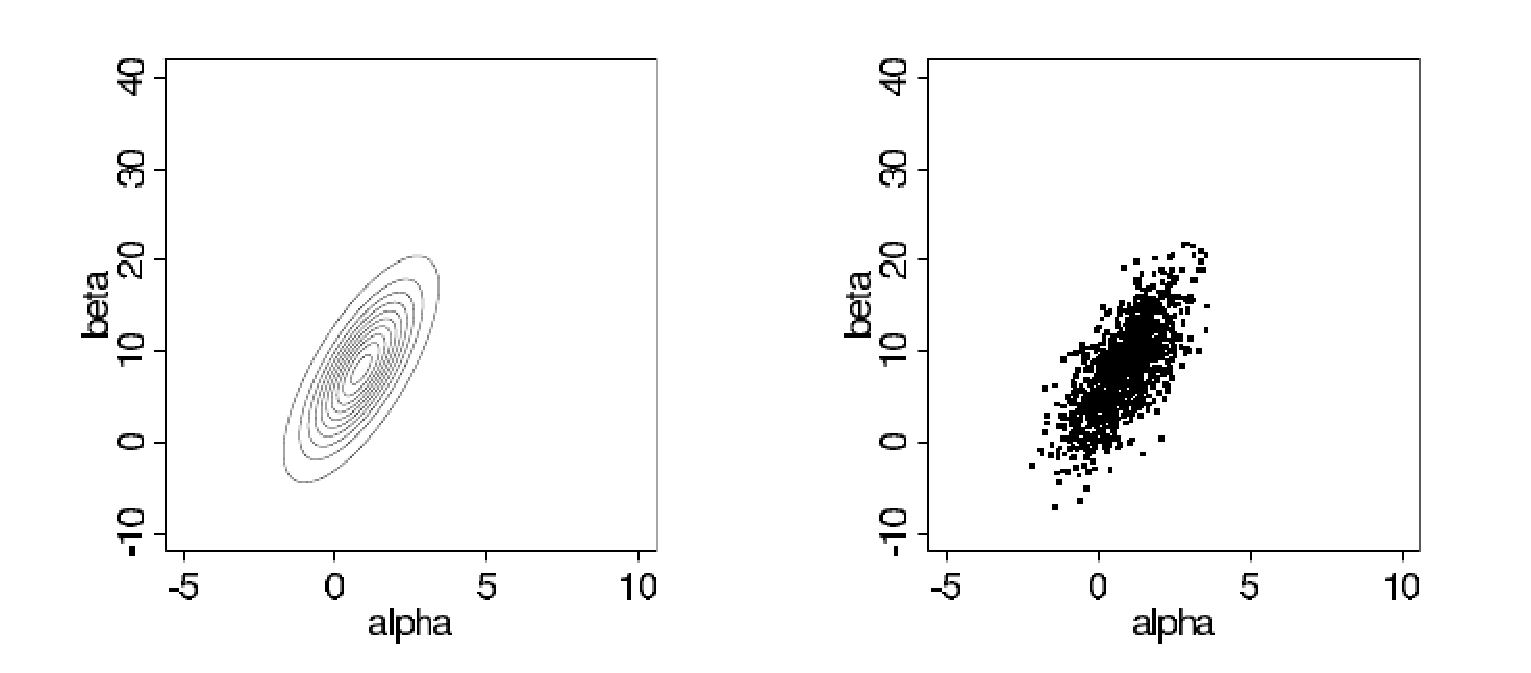
\includegraphics[scale = 0.45]{pictures/fig_4_1.eps}
\caption{Výsledky biotestu - (a) konturový graf, (b) korelační graf}
\label{fig_4_1}
\end{figure}

\subparagraph{Aposteriorní rozdělení LD50 s využitím normální aproximace parametrů $(\alpha, \beta)$.}

Výběr 1~000 pozorování náhodně vygenerovaných z normální aproximace aposteriorního rozdělení lze použít také pro odhad pravděpodobnosti $p(\beta > 0)$ a LD50 podmíněně na $\beta > 0$. Z 1~000 pozorování již 950 splňuje $\beta > 0$.
\begin{figure}[htp]
\centering
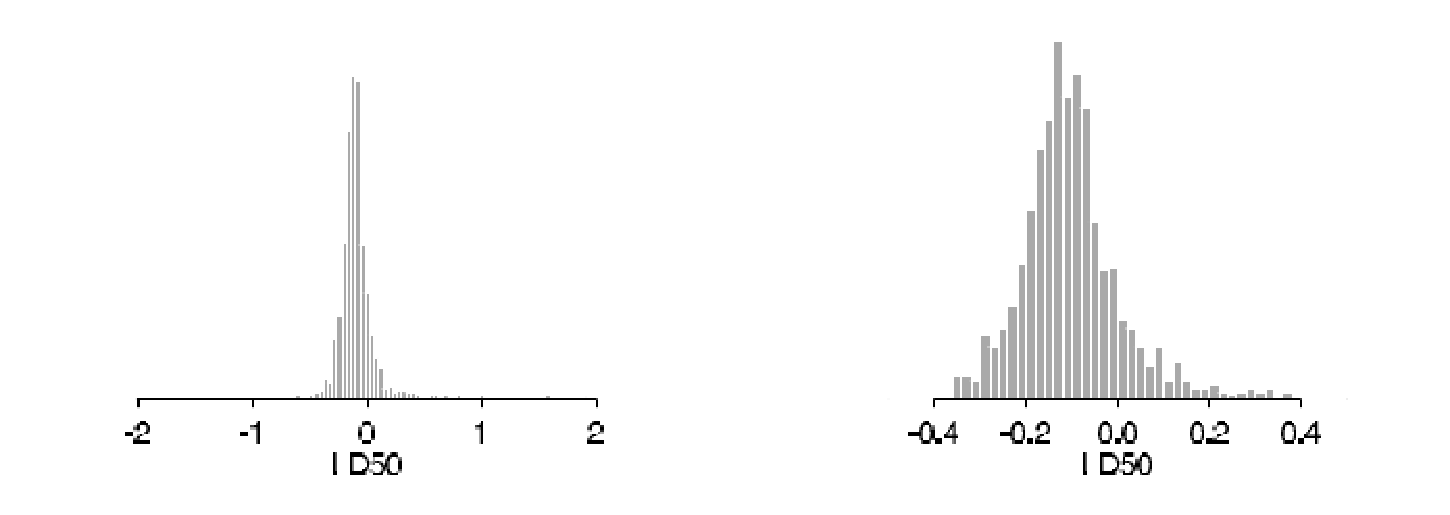
\includegraphics[scale = 0.45]{pictures/fig_4_2.eps}
\caption{Výsledky biotestu - (a) konturový graf, (b) korelační graf}
\label{fig_4_2}
\end{figure}
Obrázek 4.2a ilustruje histogram LD50 hodnot bez některých extrémních hodnot v obou chvostech.\footnote{Pokud bychom extrémní hodnoty v grafu ponechali, bylo by jeho měřítko zdeformované do té míry, že by byl nečitelný.} Obrázek 4.2b pak představuje výřez z 4.2a v okolí módu. Oba histogramy jsou centrovány přibližně kolem stejného bodu jako 3.3, nicméně vykazují mnohem vyšší volatilitu a to z důvodu vyšší pravděpodobnosti, že je skutečná hodnota parametru $\beta$ blízká nule.

Aposteriorní rozdělení založené na normální aproximaci je tedy podobné skutečnému aposteriornímu rozdělení. Nicméně, s ohledem na malou velikost náhodného výběru, je skutečné aposteriorní rozdělení výrazně více sešikmené než jeho normální aproximace, která je založená na předpokladu náhodného výběru velkého rozsahu. Proto má skutečné aposteriorní rozdělení LD50 mnohem kratší chvosty než je tomu v případě aposteriorního rozdělení založeného na normální aproximaci.

\section{Výběr velkého rozsahu}

\subsection{Úvod do problematiky}

Základním nástrojem Bayesiánské inference pro výběry velkého rozsahu je předpoklad asymptotické normality aposteriorního rozdělení. Asymptotická normalita je založena na myšlence, že s tím, jak podkladový proces generuje stále více nových dat, se aposteriorní rozdělení parametrového vektoru $\theta$ stále více blíží vícerozměrnému normálnímu rozdělení, i když skutečné pravděpodobností rozdělení dat nespadá pod uvažovanou parametrickou rodinu pravděpodobnostních rozdělení. Tento závěr lze nejsnáze aplikovat na pozorování $y_1, ..., y_n$, která jsou nezávislá a pocházejí ze společného pravděpodobnostního rozdělení $f(y)$.

Předpokládejme, že data jsou modelována pomocí parametrické rodiny $p(y|\theta)$ s apriorním rozdělením $p(\theta)$.  Jestliže je skutečné pravděpodobnostní rozdělení dat pokryté uvažovanou parametrickou rodinou, tj. jestliže $f(y) = p(y|\theta_0)$ pro určité $\theta_0$, pak je díky asymptotické normalitě splněn předpoklad konzistence. To znamená, že aposteriorní rozdělení konverguje k bodu, který představuje skutečnou hodnotu parametru $\theta_0$ s tím, jak $n \rightarrow \infty$. Pokud skutečné rozdělení uvažovanou parametrickou rodinou pokryté není, skutečné hodnoty $\theta_0$ nemusí být dosaženo - její roli přebírá hodnota $\theta_0$, pro kterou je rozdělení $p(y|\theta)$ nejbližší skutečnému rozdělení $f(y)$.

\subsection{Asymptotická normalita a konzistence}

Lze dokázat, že při splnění určitých předpokladů\footnote{Zejména se jedná o předpoklad, že věrohodnostní funkce je spojitá funkce v parametru $\theta$ a že $\theta_0$ neleží na hranici parametrového prostoru.} se aposteriorní rozdělení parametru $\theta$ blíží normálnímu rozdělení se střední hodnotu $\theta_0$ a rozptylem $\big(nJ(\theta_0)\big)^{-1}$ s tím, jak $n \rightarrow \infty$. Zjednodušeně lze tento závěr chápat v kontextu Taylorova rozvoje (4.1) logaritmu aposteriorní hustoty centrované na aposteriorní mód $\hat{\theta}$. Lze dokázat, že aposteriorní mód $\hat{\theta}$ je konzistentním odhadem skutečné hodnoty parametru $\theta_0$, tj. že a aposteriorní rozdělení $p(\theta|y)$ se koncentruje stále více a více kolem $\theta_0$ a že vzdálenost $|\hat{\theta} - \theta_0|$ se blíží nule s tím, jak $n \rightarrow \infty$.

S pomocí $p(\theta|y) = p(\theta) p(y|\theta)$ můžeme kvadratický člen (4.1) přepsat do tvaru
\begin{equation}
\Big[\frac{d^2}{d \theta^2} \ln\big(p(\theta|y)\big)\Big]_{\theta = \hat{\theta}} = \Big[\frac{d^2}{d \theta^2} \ln\big(p(\theta)\big)\Big]_{\theta = \hat{\theta}} + \sum_{i = 1}^n \Big[\frac{d^2}{d \theta^2} \ln\big(p(y_i|\theta)\big)\Big]_{\theta = \hat{\theta}}.
\end{equation}
Na tento člen, který je funkcí parametru $\theta$, lze nahlížet jako na součet konstanty a sumy $n$ členů, jejichž střední hodnota je pro skutečnou výběrovou distribuci $p(y|\theta)$ přibližně $-J(\theta_0)$, pokud je aposteriorní mód $\hat{\theta}$ dostatečně blízko skutečné hodnotě parametru $\theta_0$.\footnote{Předpokládáme, že $f(y) = p(y|\theta_0)$ pro určitou hodnotu $\theta_0$.} Proto lze pro velká $n$ aproximovat sešikmení logaritmu aposteriorního rozdělení Fisherovou informací v bodě $\hat{\theta}$.

Výše uvedené lze shrnout tak, že v kontextu zvolené pravděpodobnostní rodiny se pro velká $n$ (a) aposteriorní mód $\hat{\theta}$ limitně blíží skutečné hodnotě $\theta_0$ uvažovaného parametru a (b) sešikmení aposteriorního rozdělení se blíží $nJ(\hat{\theta})$. Dále platí, že pro $n \rightarrow \infty$ dominuje věrohodnostní funkce nad apriorním rozdělením, a proto lze použít pouze věrohodnostní funkci, abychom získali mód a sešikmení pro účely konstrukce normální aproximace.

\subsection{Dominance věrohodnostní funkce nad apriorním rozdělením}

Výše popsaná asymptotická vlastnost dává za pravdu intuici, že význam apriorního rozdělení klesá s tím, jak se zvětšuje velikost vzorku. Logickým důsledkem tohoto závěru je, že si v případě, kdy máme k dispozici velké množství dat, nemusíme příliš lámat hlavu s formulací apriorního rozdělení. A naopak, pokud je vzorek relativně malý, může hrát volba apriorního rozdělení velmi důležitou úlohu.

\section{Nesplnění předpokladů normální aproximace}

Pro níže uvedené případy nejsou splněny předpoklady normální aproximace, a proto má v jejich případě volba apriorního rozdělení vliv na aposteriorní inference, a to i v případě výběrů velkého rozsahu.

\subsection{Nedostatečně identifikované modely}

O modelu říkáme, že je nedostatečně identifikován, pokud je jeho věrohodnostní funkce $p(\theta|y)$ konstantní pro určité rozmezí hodnot parametru $\theta$. Pro takovéto modely neexistuje jediný bod $\theta_0$, ke kterému by aposteriorní rozdělení mohlo konvergovat.

\subsection{Nedostatečně identifikované parametry}

Uvažujme model
\begin{equation}
\begin{bmatrix}u \\ v \end{bmatrix} \sim N \Big(\begin{bmatrix}0 \\ 0 \end{bmatrix}, \begin{bmatrix} 1 & \rho\\ \rho & 1 \end{bmatrix} \Big),
\end{equation}
ve kterém je pro každý pár $(u, v)$ pozorováno pouze $u$ nebo $v$. V tomto případě je parametr $\rho$ neidentifikovaný. Pozorovaná data nám totiž neposkytují žádnou informaci o $\rho$, a proto je aposteriorní rozdělení tohoto parametru stejné bez ohledu na počet pozorování jako jeho apriorní rozdělení.

\subsection{Počet parametrů narůstá s velikostí výběru}

Pokud počet parametrů narůstá s počtem pozorování, pak výše uvedené závěry, které předpokládají fixní model $p(y_i | \theta)$, neplatí. Pro ilustraci uvažujme situaci, kdy je každému pozorování přiřazen parametr - např. $y_i \sim N(\theta_i, \sigma^2)$. Obecně platí, že parametry $\theta_i$ nelze konzistentně odhadnout, pokud se objem dat pro každé pozorování nezvyšuje ruku v ruce s počtem jednotek $i$.

Stejně jako v případě nedostatečně identifikovaných modelů nebude aposteriorní rozdělení parametru $\theta_i$ konvergovat k jeho skutečné hodnotě, pokud nová data nepřinesou také novou informaci o $\theta_i$. V tomto konkrétním případě aposteriorní rozdělení nekonverguje k určitému bodu, protože parametrický prostor neustále narůstá v důsledku zvyšující se dimensionality parametru $\theta$.

\subsection{Zaměnitelné parametry}

Uvažujme směsný normální model s nezávislými daty $y_1, ..., y_n$ z identického pravděpodobnostního rozdělení a parametrickým vektorem $\theta = (\mu_1, \mu_2, \sigma_1^2, \sigma_2^2, \lambda)$, kde
\begin{equation}
p(y_i|\mu_1, \mu_2, \sigma_1^2, \sigma_2^2, \lambda) = \lambda \frac{1}{\sqrt{2 \pi} \sigma_1}e^{-\frac{1}{2 \sigma_1^2}(y_i - \mu_1)^2} + (1 - \lambda) \frac{1}{\sqrt{2 \pi} \sigma_2}e^{-\frac{1}{2 \sigma_2^2}(y_i - \mu_2)^2}.
\end{equation}
Pokud prohodíme hodnoty v párech $(\mu_1, \mu_2)$ a $(\sigma_1^2, \sigma_2^2)$ a vyměníme $\lambda$ za $(1 - \lambda)$, nebude to mít vliv na věrohodnostní funkci. Aposteriorní rozdělení takovéhoto modelu tak má alespoň dva módy a skládá se ze dvou rozdělení, která jsou vzájemně zrcadlová, a proto nekonverguje do jednoho bodu a to bez ohledu na počet pozorování. Tento problém lze odstranit omezením parametrického prostoru tak, abychom odstranili případné duplicity - např. v našem případě lze parametrický prostor omezit podmínkou $\mu_1 \le \mu_2$.

\subsection{Neohraničená věrohodnostní funkce}

Jestliže je věrohodnostní funkce neohraničená (unbounded), pak v rámci parametrického prostoru nemusí existovat aposteriorní mód, což je v rozporu s předpokladem normální aproximace. Pro ilustraci uvažujme předchozí směsný normální model. Pro zjednodušení předpokládejme, že $\lambda$ je známá hodnota z otevřeného intervalu $(0, 1)$. Jestliže $\mu_1 = y_i$ pro arbitrárně zvolené $y_i$ a $\sigma_1^2 \rightarrow 0$, pak se věrohodnostní funkce blíží nekonečnu. Jak se $n$ blíží nekonečnu, narůstá počet módu věrohodnostní funkce. Jestliže je apriorní rozdělení parametru $\sigma_1^2$ uniformní a $\sigma_2^2$ se nachází poblíž nuly, narůstá také počet módů aposteriorního rozdělení, pro které neexistují odpovídající normální aproximace. Pokud je apriorní rozdělení proporcionální k $\frac{1}{\sigma_1^2 \sigma_2^2}$, je více pravděpodobnostní masy koncentrováno v okolí nuly, což má za následek ještě větší `explozi' aposteriorního rozdělení v tomto bodě.

K výše popsané situaci však v praxi dochází pouze zřídka, protože neohraničená věrohodnostní funkce je často důsledkem nerealistických podmínek v rámci modelu.

\subsection{Nevlastní aposteriorní rozdělení}

Uvažujme nenormalizované aposteriorní rozdělení získané vynásobením věrohodnostní funkce `formálním' nevlastním apriorním rozdělením. Pokud je integrál tohoto aposteriorní rozdělení roven nekonečnu, není splněn předpoklad asymptoticky normálního rozdělení, který je založen na předpokladu, že součet pravděpodobností je roven nule.

Připomeňme, že nevlastní aposteriorní rozdělení nemůže vzniknout jinak než v důsledku nevlastního apriorního rozdělení. Řešení problému je snadné - pokud zvolené apriorní rozdělení nevede k vlastnímu aposteriornímu rozdělení, je třeba zvolit jiné apriorní rozdělení, tak aby byl integrál výsledného aposteriorního rozdělení konečný.

\subsection{Apriorní rozdělení, které nezahrnuje konvergenční bod}

Jestliže $p(\theta_0) = 0$ pro nespojitý parametrický prostor nebo $p(\theta_0) = 0$ v okolí $\theta_0$ pro spojitý parametrický prostor, pak není splněn předpoklad konvergence, který je založen na dominanci věrohodnostní funkce nad apriorním rozdělením. Řešením je přiřadit všem myslitelným hodnotám parametru $\theta$ nenulovou hodnotu.

\subsection{Konvergence k hranici parametrického prostoru}

Jestliže se skutečná hodnota $\theta_0$ hledaného parametru $\theta$ nachází na hranici parametrického prostoru, pak musí být Taylorův rozvoj v daném směru `odseknutý' a výsledná normální aproximace tak nemusí být aplikovatelná a to ani v případě výběru velkého rozsahu.

Pro ilustraci uvažujme model $y_i \sim N(\theta, 1)$ s omezením $\theta \ge 0$. Předpokládejme, že se jedná o přesný model se skutečnou hodnotou parametru $\theta = 0$. Aposteriorní rozdělení parametru $\theta$ je normální centrované na $\overline{y}$ s `odseknutou' zápornou částí. Aposteriorní rozdělení parametru $\theta$ má tak pro $n \rightarrow \infty$ tvar polovičního normálního rozdělení centrovaného na bodě nula.

Uvažujme výše uvedený model, avšak tentokrát předpokládejme skutečnou hodnotu parametru $\theta = -1$, tj. hodnotu mimo parametrický prostor. Limitní aposteriorní rozdělení parametru $\theta$ má ostré maximum v bodě nula, však jeho tvar nebude ani vzdáleně připomínat tvar normálního rozdělení.

Řešením popsaného problému je uvědomit si, že se skutečná hodnota parametru nachází na hranici nebo dokonce za hranicí uvažovaného parametrického prostoru. Z tohoto důvodu je vhodné přiřadit všem myslitelným hodnotám parametru $\theta$ nenulovou pravděpodobnost.

\subsection{Chvosty pravděpodobnostního rozdělení}

Normální aproximace je často přijatelná pro většinu pravděpodobnostní masy aposteriorního rozdělení s výjimkou chvostů. Uvažujme situaci, kdy je $p(\theta | y)$ proporcionální k $e^{-c|\theta|}$ s tím, jak se $|\theta|$ blíží k nekonečnu, kde $c$ představuje konstantu.\footnote{Pro srovnání, normální rozdělení je proporcionální k $e^{-c\theta^2}$.} Pravděpodobnostní rozdělení stále konverguje k normálnímu rozdělení, avšak pro libovolný konečný vzorek velikosti $n$ tato aproximace selhává ve chvostech.

Jako další příklad uvažujme situaci, kdy je parametr $\theta$ omezený na kladné hodnoty. Pro libovolný konečný výběr bude normální aproximace přiřazovat nenulovou pravděpodobnost záporné hodnotě parametru, což je v rozporu se skutečným stavem věci.

\section{Bayesiánské inference}

\subsection{Shoda ve výběrech velkého rozsahu}

Předpokládejme, že lze aposteriorní rozdělení parametru $\theta$ aproximovat normálním rozdělením pomocí (4.2). Pak můžeme aplikovat transformaci
\begin{equation}
[I(\hat{\theta})]^{1/2}(\theta - \hat{\theta})|y \sim N(0, I),
\end{equation}
kde $\hat{\theta}$ je aposteriorní mód a $[I(\hat{\theta})]^{1/2}$ je libovolný kořen čtvercové matice $I(\hat{\theta})$. Navíc, protože $\hat{\theta} \rightarrow \theta_0$, můžeme výše uvedenou aproximaci vyjádřit pomocí $I(\theta_0)$. Jestliže je skutečné pravděpodobnostní rozdělení dat zahrnuto v uvažované třídě modelů, tj. $f(y) \equiv p(y|\theta)$ pro určité $\theta$, pak lze pro opakovaný výběr s fixním $\theta$ dokázat, že pro $n \rightarrow \infty$ platí
\begin{equation}
[I(\hat{I})]^{1/2}(\theta - \hat{\theta}) | \theta \sim N(0, I).
\end{equation}
Jedná se o závěr klasické statistické teorie, který je platný pro hodnotu odhadu $\hat{\theta}$ získaného metodou maximální věrohodnosti. Tento závěr lze snadno rozšířit také na situace, kdy je $\hat{\theta}$ rovno aposteriornímu módu. Výše uvedené výsledky implikují, že pro libovolnou funkci $(\theta - \hat{\theta})$ je aposteriorní rozdělení odvozené z (4.16) asymptoticky totožné s rozdělením získaným opakovaným výběrem z (4.17). To znamená, že 95\% aposteriorní interval parametru $\theta$ bude v 95\% případů opakovaného náhodného výběru obsahovat skutečnou hodnotu $\theta_0$.

\subsection{Bodový odhad, konzistence a efektivita odhadu}

Bodový odhad parametru $\theta$ dává smysl především v případě výběru velkého rozsahu, kdy je aposteriorní mód $\hat{\theta}$ `centrem' aposteriorního rozdělení parametru $\theta$ a nejistota reprezentovaná $nI(\hat{\theta})$ je relativně zanedbatelná. Nicméně pro výběry malého rozsahu bodový odhad parametru $\theta$ příliš smysl nedává - mnohem vhodnější je presentovat celé jeho aposteriorní rozdělení popř. hodnoty vybraných kvantilů.

O bodovém odhadu říkáme, že je konzistentní, pokud konverguje k správné hodnotě parametru s tím, jak roste velikost vzorku. Proto, pokud $f(y) \equiv p(y|\theta_0)$, je bodový odhad $\hat{\theta}$ parametru $\theta$ konzistentní, pokud jeho výběrové rozdělení konverguje k bodu $\theta_0$ s tím, jak roste velikost výběru $n$. Blízký koncept je pak tzv. asymptotická nezkreslenost, kde $\frac{E(\hat{\theta}|\theta_0)}{sd(\hat{\theta}|\theta_0)}$ konverguje k nule.\footnote{$\hat{\theta}(y)$ opět považujeme za náhodnou veličinu, jejíž pravděpodobnostní rozdělení je dáno $p(y|\theta_0)$.} Pokud rodina modelů, které kalibrujeme na pozorovaných datech, je zahrnuje skutečné pravděpodobnostní rozdělení, pak je nejen aposteriorní mód $\hat{\theta}$ ale také aposteriorní střední hodnota a medián konzistentní a asymptoticky nezkreslený a to při splnění několika relativně neomezujících regulárních podmínek.

O bodovém odhadu říkáme, že efektivní, pokud neexistuje žádná další funkce parametru $y$, která by odhadovala hodnotu parametru $\theta$ s nižší směrodatnou odchylkou, tj. $E\big((\hat{\theta} - \theta_0)^2 | \theta_0 \big)$ je nejnižší dosažitelná (aka optimální) hodnota. Efektivita odhadu $\hat{\theta}$ se měří jako poměr optimální směrodatné odchylky a skutečné směrodatné odchylky odhadu $\hat{\theta}$. Odhad je asymptoticky efektivní, pokud se tento poměr blíží jedné s tím, jak se velikost výběru $n$ blíží nekonečnu. Při splnění několika neomezujících regulárních podmínek je `střed' aposteriorního rozdělení (definovaný např. jako aposteriorní střední hodnota, medián nebo mód) asymptoticky efektivní.

\subsection{Interval spolehlivosti}

Jestliže region $C(y)$ zahrnuje $\theta_0$ v alespoň $100(1 - \alpha)\%$ případech opakovaných výběrů, pak $C(y)$ nazýváme $100(1 - \alpha)\%$ intervalem spolehlivosti parametru $\theta$. Pro ilustraci si připomeňme, že v předchozím textu jsme tvrdili, že $100(1 - \alpha)\%$ aposteriorní interval parametru $\theta$ má tu asymptotickou vlastnost, že pro opakované náhodné výběry $y$ obsahuje $100(1 - \alpha)\%$ intervalů hodnotu $\theta_0$.

\section{Bayesiánská interpretace ostatních statistických metod}

\subsection{Metoda maximální věrohodnosti a další bodové odhady}

Z pohledu Bayesiánské analýzy dat lze klasický bodový odhad často interpretovat jako aposteriorní statistiku založenou na implicitním pravděpodobnostním modelu. V případě výběru velkého rozsahu lze dokonce obhájit klasickou metodu maximální věrohodnosti pomocí Bayesiánského přístupu. Při splnění regulárních podmínek je totiž v limitě $n \rightarrow \infty$ odhad $\hat{\theta}$ získaný metodou maximální věrohodnosti  dostatečnou statistikou stejně jako aposteriorní mód, střední hodnota či medián. Jinými slovy, pro dostatečně veliké $n$ obsahuje odhad založený na metodě maximální věrohodnosti stejnou informaci o hledaném parametru $\theta$ jako samotná data.

V případě opakovaného náhodného výběru s $\theta = \theta_0$ platí
\begin{equation}
p \big(\hat{\theta}|\theta = \theta_0 \big) \approx N\big(\hat{\theta}(y)|\theta_0, (nJ(\theta_0))^{-1}\big).
\end{equation}
Výběrové rozdělení náhodné veličiny $\hat{\theta}(y)$ je tedy přibližně normální se střední hodnotou $\theta_0$ a přesností $nJ(\theta_0)$.\footnote{Abychom předešli nedorozumění, zápisem $\hat{\theta}(y)$ zdůrazňujeme, že $\hat{\theta}$ je funkcí $y$.} Pokud budeme předpokládat, že apriorní rozdělení je lokálně uniformní (nebo spojité a nenulové) v okolí skutečné hodnoty parametru $\theta$, pak prostá analýza normální střední hodnoty (viz. sekce 3.5) implikuje, že aposteriorní Bayesiánská inference má podobu
\begin{equation}
p(\theta | \hat{\theta}) \approx N(\theta | \hat{\theta}, (nJ(\hat{\theta}))^{-1}).
\end{equation}
Tento závěr přímo vyplývá z asymptotické normality, nicméně jeho odvození nepřímo skrze Bayesiánskou inferenci má poskytuje vhled do Bayesiánského odůvodnění klasické asymptotické inference založené na bodových odhadech a směrodatných odchylkách.

Závěrem připomeňme, že pro konečné $n$ není výše uvedený přístup efektivní, protože $\hat{\theta}$ není dostatečnou statistikou.

\subsection{Nezkreslené odhady}

Některé statistické metody kladou velký důraz na nezkreslenost odhadů. Odhad $\theta | y$ nazýváme nezkresleným, jestliže $E\big(\hat{\theta}(y)|\theta\big) = \theta$ pro libovolné $\theta$, kde tato střední hodnota je vypočtena pomocí $p(y|\theta)$. Z pohledu Bayesiánského přístupu je požadavek na nezkreslenost rozumný v limitě pro výběry velkého rozsahu nicméně potenciálně zavádějící v ostatních případech. Minimalizace zkreslení totiž v praxi často vede k nežádoucímu nárůstu rozptylu daného odhadu.

Obecný problém požadavku na nezkreslenost je, že v praxi je často nemožné odhadnout několik parametrů najednou tak, aby byly alespoň `přibližně' nezkreslené.

\subsubsection{Ilustrativní příklad - predikce pomocí regrese}

Nechť parametr $\theta$ představuje výšku dospělé dcery při známé výšce $y$ její matky. Předpokládejme, že výška dcery a matky sledují sdružené normální rozdělení se střední hodnotou 160 centimetrů, shodnou směrodatnou odchylkou a korelací 0.50. Aposteriorní střední hodnota parametru $\theta$ má tedy tvar
\begin{equation}
E(\theta | y) = 160 + 0.5(y - 160).
\end{equation}
Aposteriorní střední hodnota však není nezkresleným odhadem parametru $\theta$ ve smyslu opakovaného výběru $y$ pro fixované $\theta$. Pro danou výšku dcery $\theta$ má výška matky $y$ střední hodnotu $E(y | \theta) = 160 + 0.50(\theta - 160)$. Proto je v případě opakovaného výběru $y$ při fixovaném $\theta$ aposteriorní střední hodnota rovna $160 + 0.25(\theta - 160)$ a je zkreslená směrem ke střední hodnotě 160. Naopak podmíněný odhad
\begin{equation}
\hat{\theta} = 160 + 2(y - 160)
\end{equation}
je nezkreslený pro opakovaný výběr $y$. Odhad $\hat{\theta}$ bohužel nedává smysl pro hodnoty $y$ různé od 160. Pokud je matka např. o 10 centimetrů vyšší než průměrně vysoká žena, je dle tohoto odhadu její dcera o 20 centimetrů vyšší než průměr.

V tomto jednoduchém případě, ve kterém parametr $\theta$ sleduje zvolené populační rozdělení, by nebayesiánský statistik nepoužil $\hat{\theta}$ jako nezkreslený odhad. Namísto toho by tento problém `překlasifikoval' jako predikci.

\subsection{Intervaly spolehlivosti}

I pro výběry malého rozsahu jsou Bayesiánské $(1 - \alpha)\%$ aposteriorní intervaly spolehlivosti často blízké $(1 - \alpha)\%$ intervalům spolehlivosti pro opakované výběry podmíněné $\theta$. Nicméně existují intervaly spolehlivosti, které jsou založeny čistě na teorii výběru, a které jsou zcela odlišné od Bayesiánských pravděpodobnostních intervalů. Mnoho autorů ukázalo, že obecná teorie založená na nepodmíněném chování může často vést k neintuitivním výsledkům, jako jsou intervaly s nulovou nebo nekonečnou délkou. Jako jednoduchý příklad lze uvést interval spolehlivost, který je v 5\% případů prázdný a v 95\% případů obsahuje všechna reálná čísla. Tím je zajištěno, že tento interval v 95\% případů zahrnuje skutečnou hodnotu parametru $\theta$, protože v 95\% případů zahrnuje všechna reálná čísla. Tento příklad nemá za cíl zpochybnit přínos intervalů spolehlivosti, ale spíše ukázat, že samotná konvergence nezaručuje smysluplné inference.

\subsection{Testování hypotéz}

Pokud má Bayesiánská analýza vést k nenulové aposteriorní pravděpodobnosti pro nulovou hypotézu o bodovém odhadu, musíme nejprve formulovat apriorní rozdělení daného parametru tak, aby apriorní pravděpodobnost platnosti této hypotézy byla také nenulová. V případě spojitého parametru lze takové apriorní rozdělení nalézt poměrně snadno. Největší problémy s interpretací výsledků testování hypotéz je obvykle dáno formulací nulové resp. alternativní hypotézy ve tvaru $H_0: \theta = \theta_0$ resp. $H_1: \theta \ne \theta_0$. V případě spojitého parametru $\theta$ (definovaného např. jako rozdíl dvou středních hodnot) nedává nulová hypotéza $H_0: \theta = 0$ povětšinou příliš smysl a spíše nás zajímá pravděpodobnostní rozdělení popř. odpovídající interval odhadu parametru $\theta$.

Řada jednoduchých testů může být chápána jako analogie aposteriorní pravděpodobnosti pro neinformativní apriorní rozdělení. Např. předpokládejme, že pozorujeme $y = 1$ z modelu $y \sim N(\theta, 1)$ s apriorním uniformním rozdělením pro parametr $\theta$. Nemůžeme zamítnout hypotézu $\theta = 0$, protože jednostranná $p$-hodnota je 0.16 a dvoustranná $p$-hodnota je 0.32, tj. v obou případech vyšší než obvyklá hraniční hodnota 0.05. Na druhou stranu, pravděpodobnost $\theta > 0$ je 84\%, což je více informativní údaj než pouhý verdikt o zamítnutí či nezamítnutí nulové hypotézy.

\subsection{Vzájemné porovnání vícero parametrů}

Uvažujme nezávislá měření $y_j \sim N(\theta_j, 1)$ pro každý z $J$ parametrů, jejichž cílem je kvantifikovat rozdíly a pořadí spojitých parametrů $\theta_j$. V klasické statistice se nabízí několik metod víceúrovňového porovnání, které testují, zda-li jsou jednotlivá $\theta_j$ `významně' odlišná. V případě Bayesiánského přístupu sledují parametry $\theta_j$ sdružené pravděpodobnostní rozdělení. S jeho pomocí tak můžeme (alespoň teoreticky) určit aposteriorní pravděpodobnost každého z $J!$ možných pořadí.
\chapter{Hierarchické modely}

\section{Parametrizované apriorní rozdělení}

\subsection{Analýza jednoduchého experimentu v kontextu historických dat}

Uvažujme situaci, kdy odhadujeme parametr $\theta$ na základě dat získaných v rámci experimentu s pomocí apriorní distribuce zkonstruované na základě podobných historických experimentů. Jinými slovy, současná a historická data považujeme za náhodný výběr ze stejné populace.

\subsubsection{Ilustrativní příklad - odhad pravděpodobnosti nádoru}

Řada farmaceutických studií je prováděna na laboratorních potkanech. Předpokládejme, že potřebujeme odhadnout parametr $\theta$, který představuje pravděpodobnost výskytu nádoru ve skupině laboratorních potkanů, které není podáván lék, a proto ji označujeme jako tzv. kontrolní skupinu. Z dat lze vyčíst, že z celkového počtu 14 potkanů se u 4 objevil nádor. Přirozenou volbou pro modelování počtu nádorů je binomické rozdělení. Pro zjednodušení předpokládejme, že apriorní rozdělení parametru $\theta$ sleduje $\textit{Beta}(\alpha, \beta)$ rozdělení z odpovídající konjugátní rodiny.

\subparagraph{Fixní apriorní rozdělení.} Předpokládejme, že na základě historických dat víme, že pravděpodobnost výskytu nádoru, která je představovaná parametrem $\theta$, sleduje přibližně beta rozdělení se známou střední hodnotou a směrodatnou odchylkou. Pokud v minulosti proběhlo několik podobných experimentů, lze z historických dat vypočíst střední hodnotu a směrodatnou odchylku a na jejich základě vybrat vhodné hodnoty parametrů $\alpha$ a $\beta$ apriorního rozdělení.

\subparagraph{Odhad populačního rozdělení na základě historických dat.} Uvažujme historická data ze 70 podobných experimentů uvedených v tabulce na obrázku 5.1.
\begin{figure}[htp]
\centering
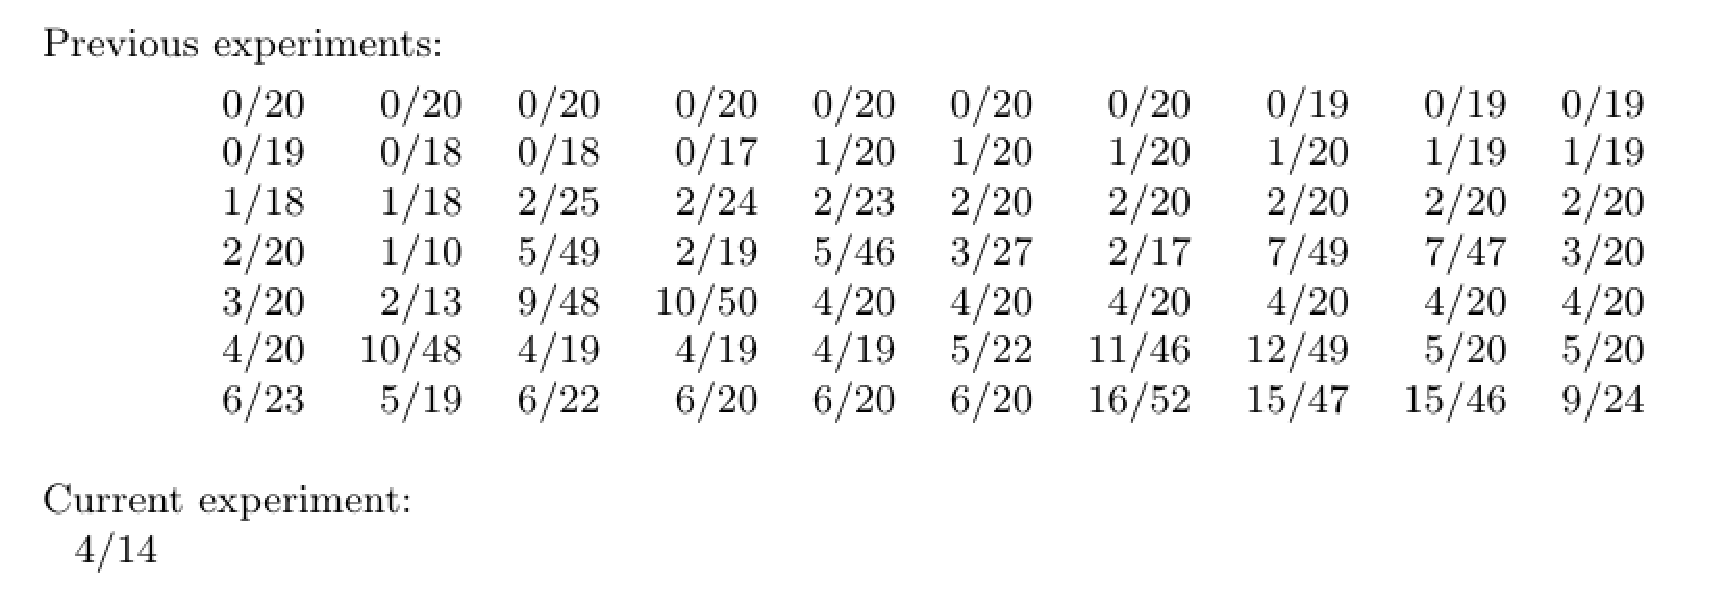
\includegraphics[scale = 0.45]{pictures/tbl_5_1.eps}
\caption{Výskyt nádoru u kontrolní skupiny potkanů; údaje jsou zobrazeny ve tvaru $\frac{\textit{počet nádorů ve skupině}}{\textit{velikost skupiny}}$.}
\label{tbl_5_1}
\end{figure}
V případě $j$-tého experimentu budeme počet nádorů označovat veličinou $y_j$ a velikost skupiny veličinou $n_j$. Počet nádorů $y_j$ budeme modelovat jako vzájemně nezávislé výběry z binomického rozdělení pro známé $n_j$ a hodnotu parametru $\theta_j$, která jsou specifické pro daný experiment. Pokud budeme předpokládat, že apriorní rozdělení $\textit{Beta}(\alpha, \beta)$ je vhodným popisem populačního rozdělení parametrů $\theta_j$, můžeme použít tzv. hierarchický model, který je schématicky znázorněn na obrázku 5.2. Index 1 až 70 představuje historické experimenty; index 71 pak představuje aktuální experiment.
\begin{figure}[htp]
\centering
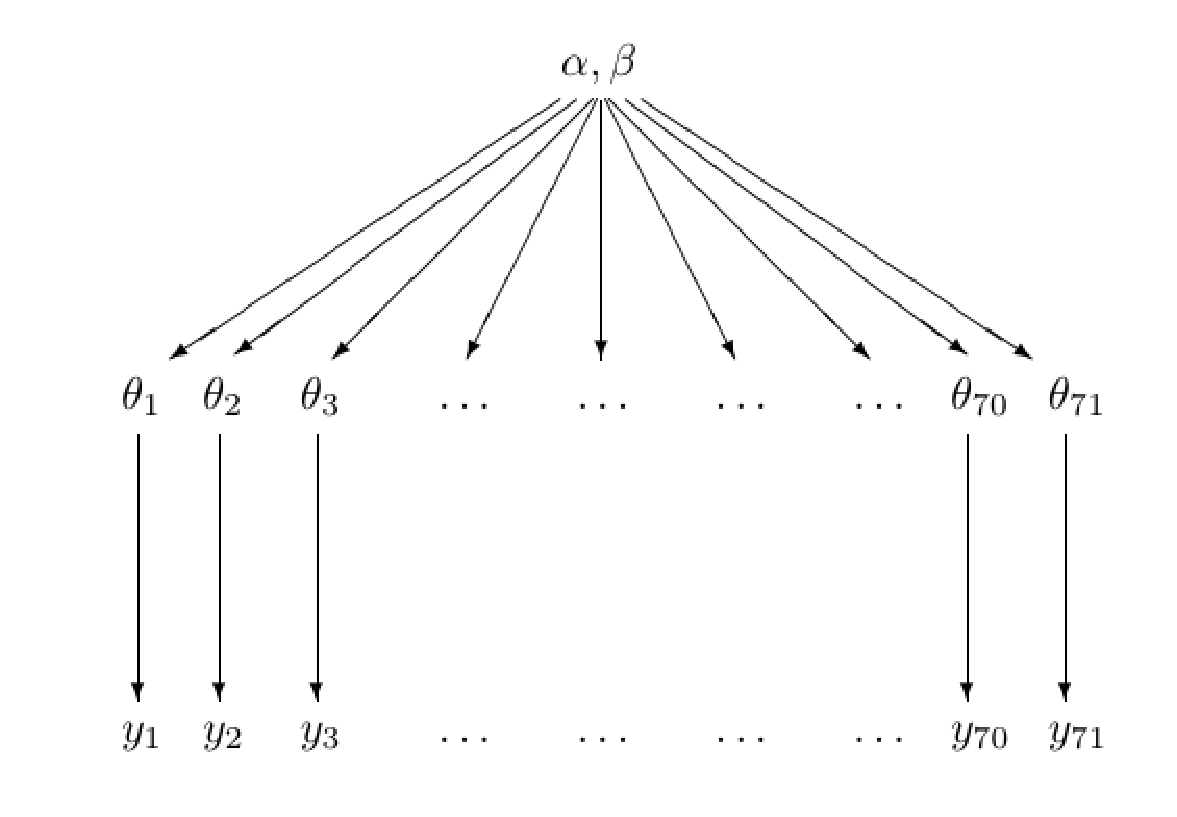
\includegraphics[scale = 0.45]{pictures/fig_5_1.eps}
\caption{Struktura hierarchického modelu pro ilustrativní příklad odhadu rizika nádoru.}
\label{fig_5_1}
\end{figure}
Střední hodnota a směrodatná odchylka parametru $\theta$ odhadnuté z historických dat jsou 0.136 a 0.103, čemuž odpovídá apriorní rozdělení $\textit{Beta}(1.4, 8.6)$. Tento jednoduchý odhad apriorního rozdělení pak odpovídá aposteriornímu rozdělení $\textit{Beta}(5.4, 18.6)$ pro aktuální parametr $\theta_{71}$. Aposteriorní střední hodnota a směrodatná odchylka parametru $\theta_{71}$ jsou tak 0.223 a 0.083.\footnote{Apriorní data způsobila, že aposteriorní střední hodnota je výrazně nižší než poměr nádorů v rámci aktuálního experimentu, tj. $4 / 14 = 0.286$. Historická zkušenost nám totiž říká, že počet nádorů v aktuálním experimentu je nezvykle vysoký.}

Je třeba zdůraznit, že výše uvedená analýza předpokládá, že historické parametry $\theta_1$ až $\theta_{70}$ a současný parametr $\theta_{71}$ pocházejí se stejného pravděpodobnostního rozdělení. Pokud existuje oprávněný důvod zpochybňující tento předpoklad, mohou být závěry výše uvedené analýzy zavádějící.

V předchozím textu jsme použili 70 historických experimentů ke konstrukci apriorního rozdělení parametru $\theta_{71}$. Toto apriorní rozdělení však můžeme, alespoň teoreticky, použít také k získání Bayesiánských inferencí parametrů $\theta_1$ až $\theta_{70}$. S tímto přístupem se však pojí několik praktických problémů.
\begin{itemize}
\item Pokud bychom apriorní rozdělení použili také pro odvození inferencí historickým experimentů, pak bychom data z těchto experimentů použili dvakrát. To by mělo za následek nadhodnocení přesnosti takto získaných odhadů.
\item Odhad $\alpha$ a $\beta$ je do určité míry arbitrární. Použití bodového odhadu těchto parametrů pak ignoruje část aposteriorní nejistoty.
\item V návaznosti na předchozí bod se také můžeme ptát, zda-li mají být parametry $\alpha$ a $\beta$ vůbec odhadovány. Tyto parametry jsou totiž součástí apriorního rozdělení a je tak otázkou, zda-li mají být v souladu s logikou Bayesiánské inference známy před tím, než máme k dispozici data ze současného experimentu.
\end{itemize}

\subsection{Kombinování informací}

Navzdory výše uvedeným problémům je smysluplnější odhadnout populační rozdělení na základě všech dat, které tak vstupují do odhadu každého jednotlivého $\theta_j$, spíše než odhadnout všech 71 hodnot $\theta_j$ samostatně.

Uvažujme parametry $\theta_{26}$ a $\theta_{27}$, které odpovídají experimentům s dvěma pozorovanými nádory v rámci skupiny 20 potkanů. Předpokládejme, že námi uvažované apriorní rozdělení pro oba parametry je centrováno na hodnotu 0.15. Dále předpokládejme, že po dokončení analýzy dat nám bylo řečeno, že skutečná hodnota $\theta_{26}$ je rovna 0.10. To by mělo mít vliv na odhad parametru $\theta_{27}$. Na základě této nové informace bychom se mohli oprávněně domnívat, že hodnota $\theta_{27}$ je nižší, než jsme se původně domnívali, protože data pro $\theta_{26}$ a $\theta_{27}$ jsou identická. Parametry $\theta_{26}$ a $\theta_{27}$ by tak měly být s ohledem na aposteriorní rozdělení `závislé' a neměly by být posuzovány odděleně.

Pokud aplikujeme pravděpodobnostní model na celou sadu parametrů $\theta_j$ a následně provedeme Bayesiánskou analýzu na sdruženém pravděpodobnostním rozdělení všech modelových parametrů, zachováme výhody plynoucí z použití dat pro odhad apriorních parametrů a zároveň se zbavíme výše zmiňovaných nevýhod. Tato tzv. kompletní Bayesiánská analýza je popsána v sekci 5.3. Na výše uvedenou analýzu využívající data pro odhad apriorních parametrů, která je někdy nazývána empirickou Bayesiánskou analýzou, můžeme pohlížet jako aproximaci kompletní Bayesiánské analýzy.

\section{Zaměnitelnost a hierarchický model}

Uvažujme skupinu experimentů $j = 1, ..., J$, kdy experiment $j$ je charakterizován daty $y_j$ a parametrem $\theta_j$ s věrohodnostní funkcí $p(y_j|\theta_j)$. Abychom zkonstruovali sdružený pravděpodobnostní model všech parametrů $\theta$, využijeme již dříve popsané myšlenky zaměnitelnosti.

\subsection{Zaměnitelnost}

Parametry $(\theta_1, ..., \theta_J)$ jsou v rámci sdruženého pravděpodobnostního rozdělení zaměnitelné, pokud je $p(\theta_1, ..., \theta_J)$ invariantní vzhledem k permutacím indexů $(1, ..., J)$. Pokud bychom např. v našem ilustrativním příkladě neměli pro 71 experimentů k dispozici jinou informaci, než je velikost $n_j$ testovaných skupin (o kterých můžeme předpokládat, že nesouvisí s hodnotou parametru $\theta_j$), pak můžeme pro parametry $\theta_j$ použít předpoklad zaměnitelnosti.

V rámci nejjednodušší formy zaměnitelného pravděpodobnostního rozdělení má každý parametr $\theta_j$ charakter náhodného výběru z apriorního (popř. populačního) rozdělení, které je dané neznámým parametrem $\phi$, neboli
\begin{equation}
p(\theta|\phi) = \prod_{j = 1}^J p(\theta_j | \phi).
\end{equation}
Obecně platí, že $\phi$ je neznámé, a proto pravděpodobnostní rozdělení parametru $\theta$ musí odrážet naši nejistotu ohledně $\phi$, tj.
\begin{equation}
p(\theta) = \int \Big(\prod_{j = 1}^J p(\theta_j | \phi) \Big) p(\phi) d\phi.
\end{equation}

\subsection{Zaměnitelnost a nová informace}

Často se stává, že pozorování nejsou plně ale pouze částečně či podmíněně zaměnitelná.
\begin{itemize}
\item Jestliže můžeme pozorování rozřadit do skupin, můžeme zkonstruovat hierarchický model, ve kterém má každá skupina svůj vlastní podmodel, jehož parametry však neznáme. Jestliže předpokládáme, že v rámci skupiny jsou pozorování zaměnitelná, můžeme pro danou skupinu zkonstruovat apriorní rozdělení parametrů charakterizujících tuto skupinu.
\item Jestliže je pozorování $y_i$ doprovázeno dodatečnou informací $x_i$ tak, že $x_i$ a $y_i$ nejsou zaměnitelné, avšak jednotlivé dvojce $(y_i, x_i)$ zaměnitelné jsou, můžeme zkonstruovat sdružený model pro $(y_i, x_i)$ nebo podmíněný model pro $y_i|x_i$.
\end{itemize}

Obvyklý způsob modelování zaměnitelnosti nezávislých veličin je přes podmíněnou nezávislost, tj. $p(\theta_1, ..., \theta_J|x_1, ..., x_J) = \int \Big[\prod_{j = 1}^J p(\theta_j | \phi, x_j)\Big]p(\phi|x)d\phi$, kde $x = (x_1, .., x_J)$. Tímto způsobem se modely založené na zaměnitelnosti stávají univerzálně použitelné, protože každá informace, která nám umožňuje rozlišit jednotlivá pozorování, by měla být zohledněna v proměnných $x$ a $y$.

V případě našeho ilustrativní příkladu pravděpodobnosti výskytu nádoru je jedinou informací, která nám umožňuje odlišit jednotlivé experimenty, velikost skupiny $n_j$. Ačkoliv není pravděpodobné, že by velikost skupiny vysvětlovala pravděpodobnost výskytu nádoru, můžeme zkonstruovat model pro $J$ párů $(n, y)_j$. Prvním přirozeným krokem je vytvoření grafu, který bude porovnávat výskyt nádoru $y_j / n_j$ s velikostí skupiny $n_j$, s cílem zjistit případnou vazbu $y_j / n_j$ na $n_j$. Např. se mohlo stát, že některé experimenty byly prováděny na větší skupině potkanů, protože se očekávala nižší míra výskytu nádoru, tj. nižší $\theta_j$, což by se pak odrazilo na nižším $y_j / n_j$. V našem případě se však žádný takový vztah nepotvrdil.

\subsection{Námitky vůči zaměnitelnému modelu}

Je přirozené odmítat předpoklad zaměnitelnosti, protože v praxi se okolnosti, za kterých byla získána jednotlivá pozorování, často liší. Např. v případě 71 experimentů v rámci ilustrativního případu byly jednotlivé experimenty prováděny v různé době, na různých skupinách potkanů, v různých laboratořích atd. Na druhou stranu, pokud nám informace, kterou máme k dispozici, neumožňuje jednotlivá pozorování odlišit, pak neexistuje důvod, proč bychom je neměli považovat za zaměnitelná.

\subsection{Hierarchický model v kontextu Bayesiánského přístupu}

Pokud se vrátíme k problému inference, pak slovo `hierarchický' znamená, že $\phi$ je neznámý parametr s vlastním apriorním rozdělením $p(\phi)$. Aposteriorní rozdělení tak má charakter vektoru $(\phi, \theta)$. Sdružené apriorní rozdělení má pak podobu
\begin{equation}
p(\phi, \theta) = p(\phi) p(\theta | \phi),
\end{equation}
a sdružené aposteriorní rozdělení podobu
\begin{equation}
\begin{split}
p(\phi, \theta|y) & \varpropto p(\phi, \theta) p(y|\phi, \theta)\\
 & = p(\phi, \theta) p(y | \theta),
\end{split}
\end{equation}
kde výše uvedené zjednodušení je platné, protože pravděpodobnostní rozdělení dat $p(y|\phi, \theta)$ závisí pouze na parametru $\theta$; $\phi$ ovlivňuje $y$ pouze skrze $\theta$.

\subsection{Hyperapriorní rozdělení}

Abychom mohli zkonstruovat sdružené pravděpodobnostní rozdělení pro $(\phi, \theta)$, musíme nejprve přiřadit apriorní rozdělení parametru $\phi$. Pokud máme o parametru $\phi$ pouze omezené informace, můžeme použít nevlastní apriorní rozdělení, pouze se musíme ujistit, že (a) výsledné aposteriorní rozdělení má konečný integrál a (b) kvantifikovat, do jaké míry jsou naše závěry citlivé na předpoklady ohledně zvoleného apriorního rozdělení. Ve většině reálných případů bychom však měli mít k dispozici dostatek informací k tomu, abychom pro $\phi$ vytyčili rozumný parametrický prostor popř. také přiřadili vhodné apriorní rozdělení.

\subsection{Aposteriorní prediktivní rozdělení}

Hierarchické modely jsou charakterizovány jak hyperparametrem $\phi$, tak parametrem $\theta$. Existují dvě aposteriorní prediktivní rozdělení, která nás zajímají a to (1) pravděpodobnostní rozdělení budoucích pozorování $\tilde{y}$ odpovídající existujícím hodnotám $\theta_j$ a (2) pravděpodobnostní rozdělení pozorování $\tilde{y}$ odpovídající budoucímu experimentu charakterizovaného neznámou hodnotou parametrem $\theta_j$. Pro účely následující textu označujeme budoucí hodnoty parametrů $\theta_j$ jako $\tilde{\theta}$.

V našem ilustrativním příkladě může být (1) dodatečný potkan v rámci již existujícího experimentu a (2) výsledek budoucího experimentu. V prvním případě je aposteriorní prediktivní výběr založen na aposteriorní hodnotě $\theta_j$ existujícího experimentu. V druhém případě je třeba nejprve náhodně vybrat $\tilde{\theta}$ pro nový experiment z populačního rozdělení pro aposteriorní výběr $\phi$, a následně vybrat $\tilde{y}$ pro simulované $\tilde{\theta}$.

\section{Bayesiánská analýza konjugátního hierarchického modelu}

\subsection{Analytické odvození podmíněného a marginálního rozdělení}

Nejprve provedeme následující tři kroky.
\begin{enumerate}
\item Vyjádříme sdružené aposteriorní rozdělení $p(\theta, \phi | y)$ v nenormalizované podobě jako součin hyperapriorního rozdělení $p(\phi)$, populačního rozdělení $p(\theta|\phi)$ a věrohodnostní funkce $p(y | \theta)$.
\item Analyticky určíme podmíněné aposteriorní rozdělení parametru $\theta$ pro daný hyperparametr $\phi$. V případě fixního pozorování $y$ má toto rozdělení podobu funkce $\phi$, konkrétně pak $p(\theta | \phi, y)$.
\item Odhadneme $\phi$ s pomocí Bayesiánského paradigmatu, tj. získáme jeho aposteriorní rozdělení $p(\phi|y)$.
\end{enumerate}

První krok lze aplikovat relativně přímočaře. Druhý krok je poměrně snadný pro konjugátní modely, protože podmíněně na $\phi$ je populační rozdělení parametru $\theta$ nezávislý a identicky rozdělený model (5.1), takže podmíněné aposteriorní rozdělení je součinem konjugátních aposteriorních rozdělení pro jednotlivé komponenty $\theta_j$. Třetí krok lze řešit pomocí `hrubé' výpočetní síly, kdy numericky integrujeme sdružené pravděpodobnostní rozdělení přes $\theta$, tj.
\begin{equation}
p(\phi | y) = \int p(\theta, \phi | y) d \theta.
\end{equation}
V případě řady standardních modelů, které jsou založeny na normálním rozdělení, lze marginální aposteriorní rozdělení $\phi$ spočítat algebraicky s použitím podmíněné pravděpodobnosti jako
\begin{equation}
p(\phi | y) = \frac{p(\theta, \phi | y)}{p(\theta | \phi, y)}.
\end{equation}
Výše uvedený výraz lze snadno použít, protože jeho čitatel je sdružené aposteriorní rozdělení (5.4) a jeho jmenovatel je aposteriorní rozdělení $\theta$ za předpokladu známého $\phi$. Obtížnost použitelnosti (5.6) v praxi spočítá v tom, že (s výjimkou několika málo standardních konjugátních modelů) má jmenovatel $p(\theta | \phi, y)$ normalizační faktor, který závisí jak na $\phi$ tak na $y$. Při aplikaci normalizační konstanty v rámci Bayesovy věty je třeba se ujistit (a to zejména v případě hierarchických modelů), že se skutečně jedná o konstantu.

\subsection{Náhodný výběr z aposteriorního rozdělení}

Následující postup je vhodný pro náhodný výběr ze sdruženého pravděpodobnostního rozdělení $p(\theta, \phi | y)$ v případě jednoduchého hierarchického modelu, jaký uvažujeme v této kapitole.
\begin{itemize}
\item Náhodně vybereme hyperparametr $\phi$ z jeho aposteriorního marginálního rozdělení $p(\phi | y)$. Pokud má $\phi$ povahu skaláru, můžeme pro náhodný výběr použít stejnou metodu jako v kapitole 3. Pokud má $\phi$ charakter vektoru, je třeba použít sofistikovanější metodu, viz. např. část III této knihy.
\item Náhodně vybereme parametr $\theta$ z aposteriorního podmíněného rozdělení $p(\theta | \phi, y)$ pro hodnotu $\phi$ získanou v předchozím kroku. Pokud platí faktorizace $p(\theta | \phi, y) = \prod_j p(\theta_j | \phi, y)$, lze jednotlivé komponenty $\theta_j$ vybrat postupně nezávisle na sobě.
\item Prediktivní hodnoty $\tilde{y}$ lze získat z aposteriorního prediktivního rozdělení pro dané $\theta$. V závislosti na uvažovaném problému může být nejprve nutné náhodně vybrat novou hodnotu $\tilde{\theta}$ pro dané $\phi$ tak, jak bylo diskutováno na konci předchozí sekce.
\end{itemize}
Výše uvedené kroky jsou zopakovány $L$-krát s cílem získat $L$ náhodných výběrů. Na základě aposteriorní sdružené simulace $\theta$ a $\tilde{y}$ lze vypočíst aposteriorní rozdělení libovolného odhadu nebo prediktivního ukazatele.

\subsection{Aplikace modelu na pravděpodobnost výskytu nádoru}

Nyní aplikujeme Bayesiánskou analýzu na ilustrativní příklad pravděpodobnosti výskytu nádoru, který je popsán v sekci 5.1. Opět předpokládáme, že data z experimentů $j = 1, ..., J$, kde $J = 71$, sledují nezávislá binomická rozdělení
\begin{equation}
y_j \sim \textit{Bin}(n_j, \theta_j),
\end{equation}
kde $n_j$ představuje počet potkanů ve skupině. O parametrech $\theta_j$ předpokládáme, že se jedná o nezávislé výběry z beta rozdělení, tj.
\begin{equation}
\theta_j \sim \textit{Beta}(\alpha, \beta)
\end{equation}
a hyperparametrům $(\alpha, \beta)$ přiřadíme neinformativní rozdělení s ohledem na naši neznalost jejich skutečného rozdělení. Pokud se volba tohoto neinformativního hyperapriorního rozdělení z pohledu výsledné inference ukáže jako zásadní, měli bychom toto zjištění v naší studii zmínit a případně se pokusit získat další data, která by nám umožnila konstrukci `informativnějšího' apriorního rozdělení. Pokud použijeme nevlastní apriorní rozdělení pro hyperparametry $(\alpha, \beta)$, musíme zkontrolovat, že má výsledné aposteriorní rozdělení konečný integrál.

\subsubsection{Sdružené, podmíněné a marginální aposteriorní rozdělení}

Sdružené aposteriorní rozdělení všech parametrů má podobu
\begin{equation}
\begin{split}
p(\theta, \alpha, \beta | y) & \varpropto p(\alpha, \beta) p(\theta | \alpha, \beta) p(y | \theta, \alpha, \beta)\\
 & \varpropto p(\alpha, \beta) \prod_{j = 1}^J \frac{\Gamma(\alpha + \beta)}{\Gamma(\alpha) \Gamma(\beta)} \theta_j^{\alpha - 1}(1 - \theta_j)^{\beta - 1} \prod_{j = 1}^J \theta_j^{y_j}(1 - \theta_j)^{n_j - y_j}.
\end{split}
\end{equation}
Pro dané $(\alpha, \beta)$ sledují komponenty vektoru $\theta$ identická aposteriorní rozdělení, která mají formu beta rozdělení $\theta_j^A(1 - \theta_j)^B$ a sdružené rozdělení má tak tvar
\begin{equation}
p(\theta | \alpha, \beta, y) = \prod_{j = 1}^J \frac{\Gamma(\alpha + \beta + n_j)}{\Gamma(\alpha + y_j)\Gamma(\beta + n_j - y_j)} \theta_j^{\alpha + y_j - 1}(1 - \theta_j)^{\beta + n_j - y_j - 1}.
\end{equation}
Aposteriorní marginální rozdělení $(\alpha, \beta)$ můžeme získat dosazením (5.9) a (5.10) do rovnice podmíněné pravděpodobnosti (5.6), čímž získáme
\begin{equation}
p(\alpha, \beta | y) \varpropto p(\alpha, \beta) \prod_{j = 1}^J \frac{\Gamma(\alpha + \beta)}{\Gamma(\alpha)\Gamma(\beta)} \frac{\Gamma(\alpha + y_j)\Gamma(\beta + n_j - y_j)}{\Gamma(\alpha + \beta + n_j)}.
\end{equation}

\subsubsection{Standardní parametrizace a nastavení neinformativního hyperapriorního rozdělení}

Protože nemáme k dispozici informaci o pravděpodobnostním rozdělení výskytu nádoru, použijeme pro $\alpha$ a $\beta$ `obecná' hyperapriorní rozdělení. Před samotným výběrem těchto rozdělení však $\alpha$ a $\beta$ transformujeme na $logit\big(\frac{\alpha}{\alpha + \beta}\big) = \ln\big(\frac{\alpha}{\beta}\big)$ a $\ln \big(\alpha + \beta \big)$, což jsou logit střední hodnoty a logaritmus `velikosti výběru' beta rozdělení použitého pro modelování parametru $\theta$. Pomocí těchto transformací jsme střední hodnotu a `velikost výběru' převedli na interval $(-\infty, \infty)$. Jestliže přijmeme předpoklad o nezávislosti střední hodnoty a `velikosti výběru', můžeme takto transformovaným parametrům nezávislá hyperapriorní rozdělení. Pokud bychom však použili uniformní rozdělení, získali bychom nevlastní aposteriorní rozdělení, které má nekonečný integrál v limitě $(\alpha + \beta) \rightarrow \infty$. Proto v tomto konkrétním případě musíme zvolit jiný typ hyperapriorního rozdělení.

V našem ilustrativním příkladě je možné použít `neinformativní' hyperapriorní rozdělení, kterému `dominuje' věrohodnostní funkce, což vede vlastnímu aposteriornímu rozdělení. Jedním z takovýchto možných hyperapriorních rozdělení je uniformní rozdělení nad intervalem $\big(\frac{\alpha}{\alpha + \beta}, (\alpha, \beta)^{-1/2} \big)$, které po vynásobení příslušným Jacobiánem vede k
\begin{equation}
p \Big(\ln \big(\ln \frac{\alpha}{\beta}\big), \ln(\alpha + \beta) \Big) \varpropto \alpha \beta (\alpha + \beta)^{-5/2}
\end{equation}
a po převedením na původní škálu k
\begin{equation}
p(\alpha, \beta) \varpropto (\alpha + \beta)^{-5/2}.
\end{equation}

Alternativně lze použít rozdělení typu $p(\frac{\alpha}{\alpha + \beta}, \alpha + \beta) \varpropto 1$ popř. $p(\alpha, \beta) \varpropto 1$ a následně zkonstruovat kontury na základě simulace z výsledného aposteriorního rozdělení. Z těchto výsledků by mělo být patrné, zda-li aposteriorní kontury směřují do nekonečna, což indikuje, že aposteriorní rozdělení nemá konečný integrál. Stejně jako v předchozím případech, i zde je řešením volba jiného apriorního rozdělení.

Bohužel použití apriorního uniformního rozdělení pro $\big(\ln(\frac{\alpha}{\beta}), \ln(\alpha + \beta) \big)$ i nad poměrně `velkorysým' hyperparametrickým prostorem jako např. $[-10^{10}, 10^{10}] \times [-10^{10}, 10^{10}]$ není řešením, protože většina pravděpodobnostní masy je koncentrováno v regionu, kde se $\alpha$ a $\beta$ blíží nekonečnu. To odpovídá $\textit{Beta}(\alpha, \beta)$ rozdělení s nulovým rozptylem, což znamená, že všechny parametry $\theta_j$  jsou v rámci aposteriorního rozdělení totožné. Pokud věrohodnostní funkce nemá konečný integrál, pak tento problém nelze vyřešit rozšířením hyperparametrické prostoru.

\subsubsection{Výpočet marginálního aposteriorního rozdělení hyperparametrů}

Po té, co jsme odvodili pravděpodobnostní modely pro data a parametry, můžeme vypočíst marginální aposteriorní rozdělení hyperparametrů. Obrázek 5.3 zobrazuje konturový graf nenormalizovaného aposteriorního rozdělení na mřížce $\big(\ln(\frac{\alpha}{\beta}), \ln(\alpha + \beta) \big)$.
\begin{figure}[htp]
\centering
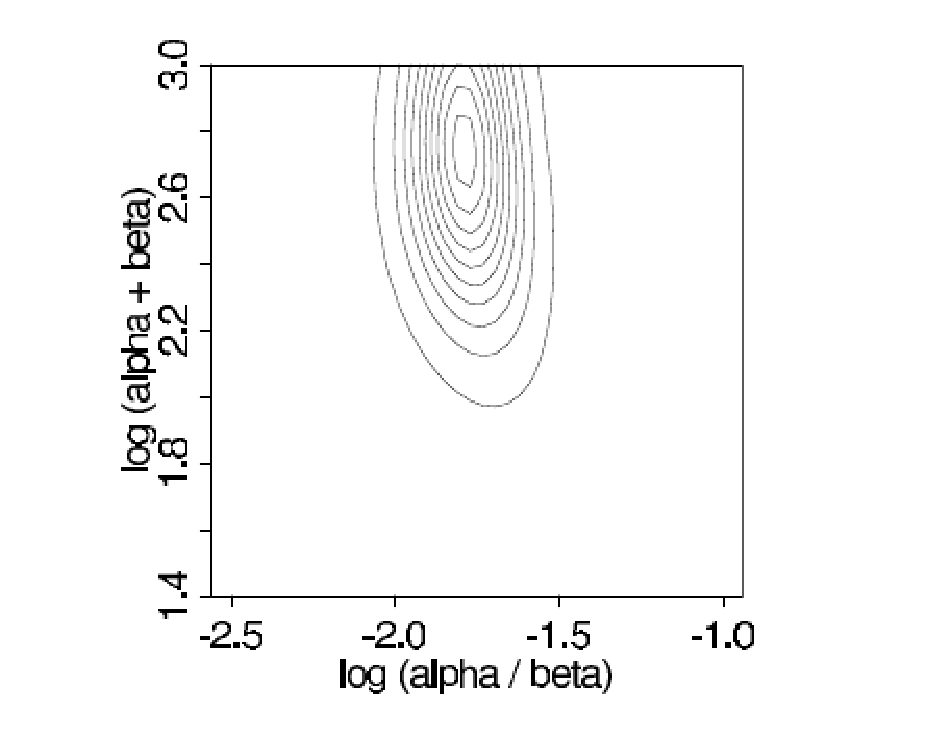
\includegraphics[scale = 0.45]{pictures/fig_5_2.eps}
\caption{První pokus o konturový graf marginálního aposteriorního rozdělení parametrů $\big(\ln(\frac{\alpha}{\beta}), \ln(\alpha + \beta) \big)$ pro ilustrativní příklad míry výskytu nádoru.}
\label{fig_5_2}
\end{figure}
Graf byl zkonstruován tak, že jsme nejprve vypočetli logaritmus pravděpodobnostního rozdělení (5.11) s využitím apriorního rozdělení (5.13) a následně vynásobili Jacobiánem s cílem získat pravděpodobnostní rozdělení $\big(\ln(\frac{\alpha}{\beta}), \ln(\alpha + \beta) \big)$. Mřížku v grafu jsme nastavili na $\big(\ln(\frac{\alpha}{\beta}), \ln(\alpha + \beta) \big) \in [-2.5, -1.0] \times [1.5, 3.0]$ vycentrovanou na bod našeho předchozího odhadu $(-1.8, 2.3)$, což odpovídá $(\alpha, \beta) \in (1.4, 8.6)$. Nakonec, abychom se vyhnuli numerickým problémům, jsme odečetli maximální hodnotu logaritmu pravděpodobnostního rozdělení od každého bodu mřížky a aplikovali exponenciálu, čímž jsme získali nenormalizované marginální aposteriorní rozdělení zobrazené v grafu.

Z výše uvedeného konturového grafu je zřejmé, že (1) mód není příliš daleko od bodového odhadu a (2) významná část marginálního aposteriorního rozdělení se nachází mimo uvažovanou hyperparametrickou mřížku. Proto přepočteme $\big(\ln(\frac{\alpha}{\beta}), \ln(\alpha + \beta) \big)$ nad mřížkou $[-2.3, -1.3] \times [1.0, 5.0]$. Výsledný graf je zachycen na obrázku 5.4a a zobrazuje téměř celé marginální aposteriorní rozdělení.
\begin{figure}[htp]
\centering
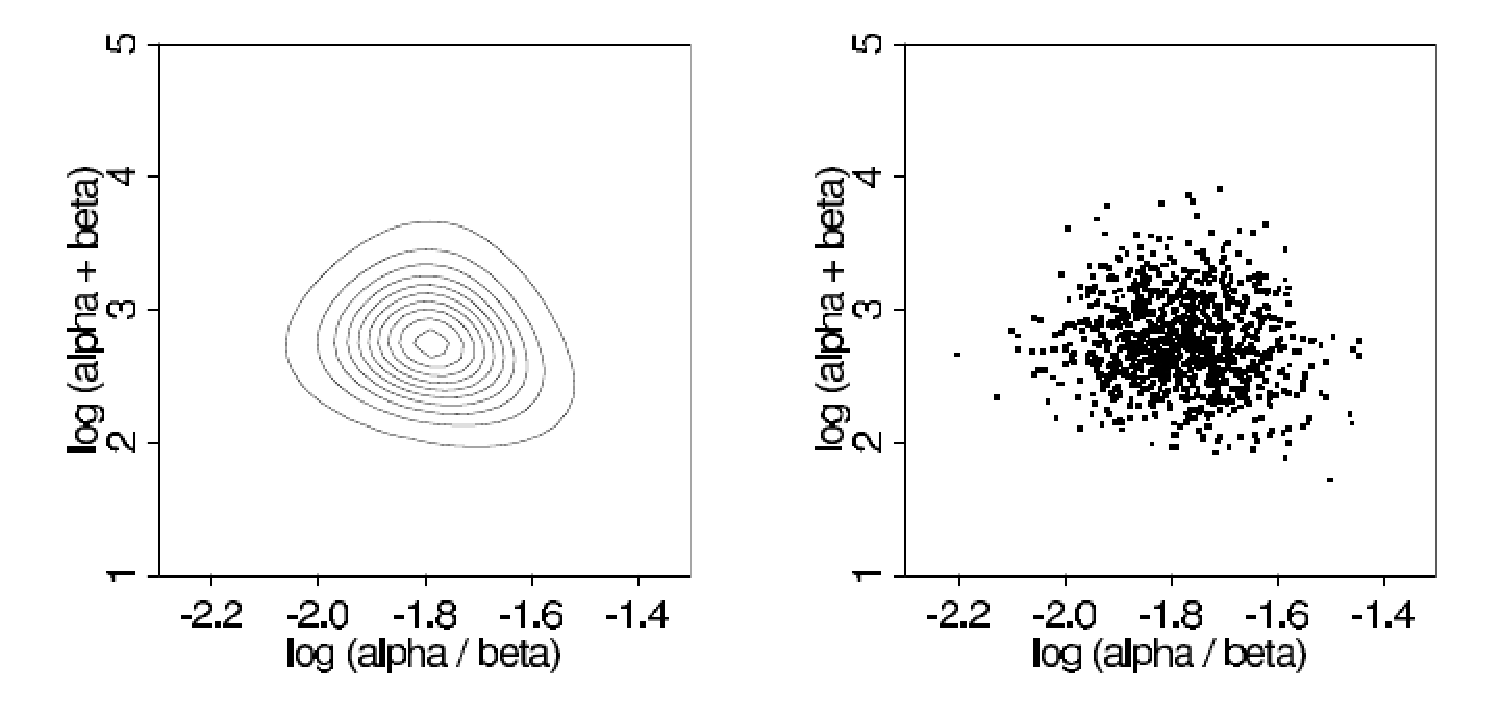
\includegraphics[scale = 0.45]{pictures/fig_5_3.eps}
\caption{(a) Konturový graf marginálního aposteriorního rozdělení parametrů $\big(\ln(\frac{\alpha}{\beta}), \ln(\alpha + \beta) \big)$ pro ilustrativní příklad pravděpodobnosti výskytu nádoru. Konturové linie jsou zobrazeny pro 0.05, 0.15, ..., 0.95 násobek hustoty pravděpodobnosti v módu. (b) Korelační diagram 1~000 náhodných výběrů $\big(\ln(\frac{\alpha}{\beta}), \ln(\alpha + \beta) \big)$ z numericky vypočteného marginálního aposteriorního rozdělení.}
\label{fig_5_3}
\end{figure}
Graf na obrázku 5.4b pak zobrazuje 1~000 náhodných výběrů z numericky vypočteného aposteriorního rozdělení. Z obou grafů je také patrné, že po aplikaci transformací je aposteriorní rozdělení hyperparametrů přibližně symetrické okolo módu a to v rozpětí $(-1.75, 2.80)$. To odpovídá přibližně hodnotám $(\alpha, \beta) = (2.40, 14.0)$, což se do určité míry odlišuje od našich dřívějších hrubých odhadů.

Po té, co jsme vypočetli relativní aposteriorní rozdělení nad mřížkou, která pokrývá efektivní rozpětí hyperparametrů $(\alpha, \beta)$, můžeme toto rozdělení aproximovat schodovou funkcí a následně normalizovat tak, aby součet jejích pravděpodobnostní byl roven jedné.

V dalším kroku pak můžeme vypočíst aposteriorní momenty založené na mřížce $\big(\ln(\frac{\alpha}{\beta}), \ln(\alpha + \beta) \big)$, kdy např. $E(\alpha | y)$ je odhadnuto jako
\begin{equation}
E(\alpha | y) = \sum_{\ln\big(\frac{\alpha}{\beta}\big), \ln(\alpha + \beta)} \alpha \cdot p\Big(\ln\big(\frac{\alpha}{\beta}\big), \ln(\alpha + \beta) | y \Big).
\end{equation}

\subsubsection{Výběr ze sdruženého aposteriorního rozdělení parametrů a hyperparametrů}

Náhodný výběr o velikosti 1~000 vzorků ze sdruženého aposteriorního rozdělení pro $(\alpha, \beta, \theta_1, ..., \theta_J)$ získáme následujícím způsobem.

\begin{enumerate}
\item Nejprve náhodně vybereme 1~000 vzorků $\big(\ln(\frac{\alpha}{\beta}), \ln(\alpha + \beta) \big)$ z aposteriorního rozdělení zobrazeného na obrázku 5.4. Pro výběr použijeme stejný postup jako v případě výběru $(\alpha, \beta)$ u obrázku (3.3).
\item Pro $l = 1, ..., 1~000$:
\begin{enumerate}
\item Transformujeme $l$-tý výběr $\big(\ln(\frac{\alpha}{\beta}), \ln(\alpha + \beta) \big)$ na $(\alpha, \beta)$ s cílem získat náhodný výběr hyperparametrů z jejich marginálního aposteriorního rozdělení.
\item Pro každé $j = 1, ..., J$ náhodně vybereme $\theta_j$ z podmíněného aposteriorního rozdělení $\theta_j | \alpha, \beta, y \sim \textit{Beta}(\alpha + y_j, \beta + n_j - y_j)$.
\end{enumerate}
\end{enumerate}

\subsubsection{Zobrazení výsledků}

Obrázek 5.5 zobrazuje aposteriorní mediány a 95\% intervaly spolehlivosti pro jednotlivá $\theta_j$ získaná pomocí simulace.
\begin{figure}[htp]
\centering
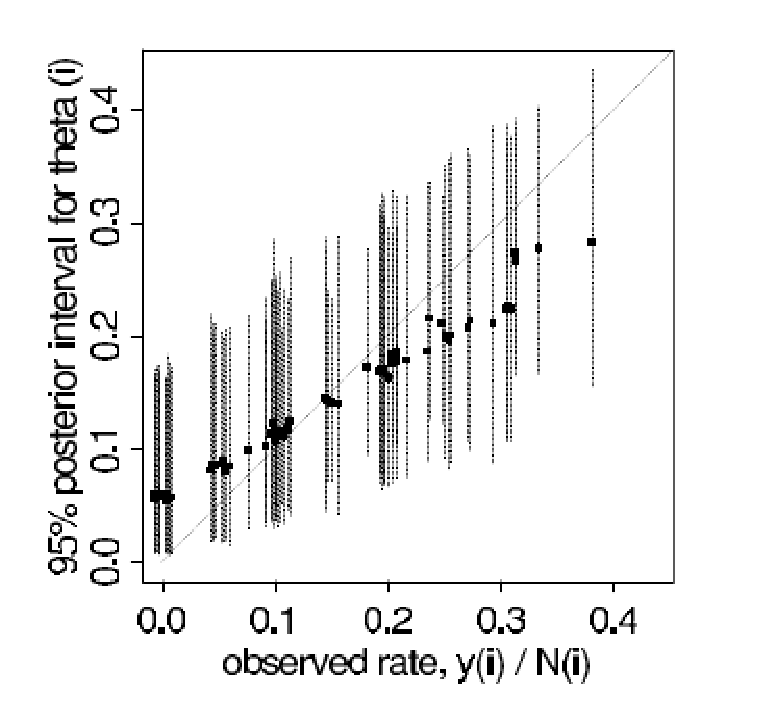
\includegraphics[scale = 0.45]{pictures/fig_5_4.eps}
\caption{Aposteriorní mediány a 95\% intervaly spolehlivosti pravděpodobnosti výskytu nádoru $\theta_j$ (vs. pozorované míry výskytu $y_j / n_j$) založené na náhodných výběrech ze sdruženého aposteriorního rozdělení.}
\label{fig_5_4}
\end{figure}
Pravděpodobnosti nádorů $\theta_j$ pro jednotlivé experimenty jsou z jejich bodových odhadů $y_j / n_j$ vychýleny směrem k střední hodnotě populačního rozdělení, která je přibližně rovna 0.14. Použitím populačního rozdělení jsme docílili, že experimenty s méně pozorováními vykazují vyšší aposteriorní rozptyl. Střední hodnoty odhadovaných parametrů $\theta_j$ jsou přibližně stejné jako v případě bodových odhadů, což není vzhledem k relativně velkému počtu experimentů překvapivé. Nicméně zásadním rozdílem je vyšší rozptyl těchto parametrů, což je odrazem aposteriorní nejistoty hyperparametrů $\alpha$ a $\beta$.

\section{Odhad zaměnitelných parametrů z normálního modelu}

\subsection{Datová struktura}

Uvažujme $J$ nezávislých experimentů, kde v rámci $j$-tého experimentu odhadujeme parametr $\theta_j$ na základě $n_j$ nezávislých pozorování $y_{ij}$ z normálního rozdělení se známým rozptylem $\sigma^2$, tj.
\begin{equation}
y_{ij} | \theta_j \sim N(\theta_j, \sigma^2)
\end{equation}
pro $i = 1, ..., n_j$ a $j = 1, ..., J$. Pro každý jednotlivý experiment definujme výběrovou střední hodnotu
\begin{equation}
\overline{y}_{\cdot j} = \frac{1}{n_j} \sum_{i = 1}^{n_j} y_{ij}
\end{equation}
a výběrový rozptyl
\begin{equation}
\sigma^2_j = \frac{\sigma^2}{n_j}.
\end{equation}
Věrohodnostní funkci $\theta_j$ pak můžeme zapsat s pomocí dostatečné statistiky $\overline{y}_{\cdot j}$ jako
\begin{equation}
\overline{y}_{\cdot j} | \theta_j \sim N(\theta_j, \sigma^2_j).
\end{equation}
V následujícím textu této kapitoly budou všechny výrazy implicitně podmíněny známými hodnotami $\sigma_j^2$.

\subsection{Konstrukce apriorního rozdělení pro účely pragmatických úvah}

Zamysleme se nad tím, jaký typ aposteriorních odhadů může být přijatelný pro $\theta$ při daných datech $(y_{ij})$. Nejjednodušší přístup je odhadnout $\theta_j$ pomocí $\overline{y}_{\cdot j}$, tj. pomocí průměru $j$-tého experimentu. Nicméně se může stát, že budeme mít např. $J = 20$ experimentů s pouze $n_j = 2$ pozorováními na skupinu. V tomto případě můžeme odhadnout $\theta_j$ pomocí tzv. sdíleného odhadu (pooled estimate)
\begin{equation}
\overline{y}_{\cdot \cdot} = \frac{\sum_{j = 1}^J \frac{1}{\sigma_j^2}\overline{y}_{\cdot j}}{\sum_{j = 1}^J \frac{1}{\sigma^2_j}}.
\end{equation}

Abychom rozhodli, který odhad použít, lze aplikovat $F$ test z klasické statistiky na rozdíly mezi středními hodnotami jednotlivých skupin. Pokud se neprokáže, že střední hodnoty jsou v rámci $J$ skupin statisticky významně odlišné, lze použít sdílený odhad $\overline{y}_{\cdot \cdot}$. Následující tabulka shrnuje analýzu rozptylu, kde $\tau^2$ představuje rozptyl parametrů $\theta_1, ..., \theta_J$. Pro zjednodušení předpokládáme $n_j = n$ a $\sigma_j^2 = \sigma^2 / n$ pro všechna $j$.
\begin{figure}[htp]
\centering
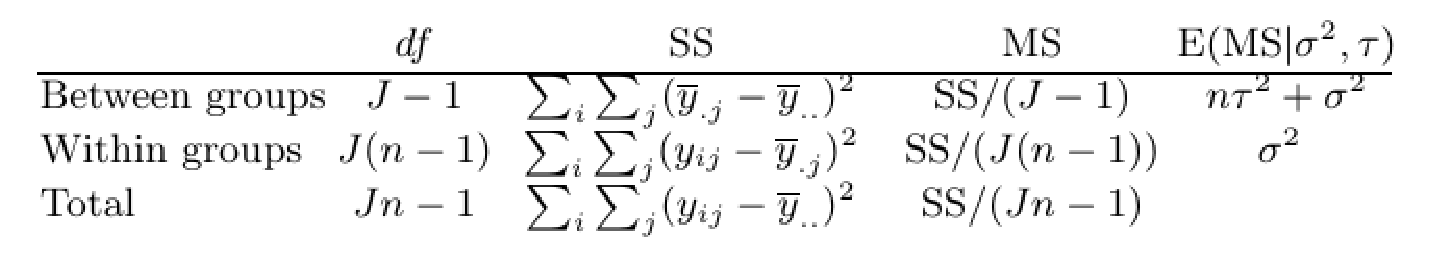
\includegraphics[scale = 0.45]{pictures/tbl_5_2.eps}
\caption{Tabulka analýzy rozptylu}
\label{fig_5_2}
\end{figure}
V klasické analýze rozptylu se vypočte sloupec součtů čtverců (SS - sum of squares) a sloupec průměru čtverců (MS - mean square) a následně se použije meziskupinový a vnitroskupinový průměr čtverců pro odhad $\tau$. Pokud je poměr meziskupinového a vnitroskupinového průměru čtverců výrazně vyšší než 1.0, pak na základě této analýzy rozptylu budeme jednotlivá $\theta_j$ odhadovat zvlášť, tj. $\hat{\theta}_j = \overline{y}_{\cdot j}$. Pokud je však poměr průměrů čtverců statisticky nevýznamný, odhadujeme $\theta_j$ jednou hodnotou $\overline{y}_{\cdot \cdot}$ pro všechna $j$. Alternativně můžeme použít vážený průměr těchto dvou přístupů, tj.
\begin{equation}
\hat{\theta}_j = \lambda_j \overline{y}_{\cdot j} + (1 - \lambda_j) \overline{y}_{\cdot \cdot},
\end{equation}
kde $\lambda_j$ představuje váhu mezi $0$ a $1$. Na tento přístup lze také pohlížet jako na zobecnění dvou předchozích přístupů, které jsou reprezentovány krajními hodnotami $\lambda = 0$ a $\lambda = 1$.

Následující body shrnují, jaké typy apriorních modelů vedou k jakým typům aposteriorních odhadů.
\begin{enumerate}
\item Odhad $\hat{\theta}_j = \overline{y}_{\cdot j}$ je aposteriorní střední hodnotou, pokud $J$ hodnot $\theta_j$ sleduje nezávislé apriorní uniformní rozdělení nad intervalem $(-\infty, \infty)$.
\item Odhad $\hat{\theta} = \overline{y}_{\cdot \cdot}$ je aposteriorní střední hodnotou, pokud je všech $J$ hodnot $\theta_j$ shodných s uniformním apriorním rozdělením pro společné $\theta$.
\item Vážený průměr dvou výše uvedených přístupů je aposteriorní střední hodnotou, pokud $J$ hodnot $\theta_j$ sleduje nezávislá a identická apriorní normální rozdělení.
\end{enumerate}

\subsection{Hierarchický model}

Z důvodu konjugace předpokládáme, že jsou parametry $\theta_j$ náhodně vybrány z normálního rozdělení popsaného hyperparametry $(\mu, \tau)$
\begin{equation}
\begin{split}
p(\theta_1 ..., \theta_J | \mu, \tau) = \prod_{j = 1}^J N(\theta_j | \mu, \tau^2)\\
p(\theta_1, ..., \theta_J) = \int \prod_{j = 1}^J \big[N(\theta_j | \mu, \tau^2)\big]p(\mu, \tau)d(\mu, \tau).
\end{split}
\end{equation}
To znamená, že $\theta_j$ jsou podmíněně na $(\mu, \tau)$ vzájemně nezávislá. Hierarchický model také dovoluje interpretovat jednotlivá $\theta_j$ jako náhodný výběr z populačního rozdělení tak, jak to ilustruje obrázek 5.1.

Přiřaďme hyperparametru $\mu$ neinformativní uniformní rozdělení za předpokladu znalosti $\tau$
\begin{equation}
p(\mu, \tau) = p(\mu | \tau) p(\tau) \varpropto p(\tau).
\end{equation}
Použití uniformního apriorního rozdělení je v tomto případě rozumné - vzhledem k tomu, že kombinovaná data ze všech $J$ experimentů jsou obecně velmi informativní ohledně $\mu$, můžeme si v případě apriorního rozdělení dovolit být relativně vágní. Apriorní rozdělení hyperparametru $\tau$ budeme diskutovat později.

\subsection{Sdružené aposteriorní rozdělení}

Kombinací výběrového modelu pro pozorování $y_{ij}$ a apriorního rozdělení získáme sdružené aposteriorní rozdělení všech parametrů a hyperparametrů, které můžeme vyjádřit pomocí dostatečných statistik $\overline{y}_{\cdot j}$ jako
\begin{equation}
\begin{split}
p(\theta, \mu, \tau | y) & \varpropto p(\mu, \tau) p(\tau | \mu, \tau) p(y | \theta)\\
 & \varpropto p(\mu, \tau) \prod_{j = 1}^J N(\theta_j | \mu, \tau^2) \prod_{j = 1}^J N(\overline{y}_{\cdot j} | \theta_j, \sigma_j^2),
\end{split}
\end{equation}
kde můžeme ignorovat členy, které závisí pouze na $y$ a parametrech $\sigma_j$, o kterých předpokládáme, že je známe.

\subsection{Podmíněné aposteriorní rozdělení normálních středních hodnot pro známé hyperparametry}

Stejně jako v obecné hierarchické struktuře jsou parametry $\theta_j$ v apriorním rozdělení nezávislé (pro dané $\mu$ a $\tau$) a figurují ve věrohodnostní funkci (5.15). To znamená, že podmíněné aposteriorní rozdělení $p(\theta | \mu, \tau, y)$ lze rozložit na součin $J$ komponent.

Podmíněně na hyperparametrech tak máme $J$ nezávislých neznámých středních hodnot, které sledují dané apriorní normální rozdělení, a proto můžeme nezávisle na každém $\theta_j$ aplikovat metody ze sekce 2.5. Podmíněná aposteriorní rozdělení parametrů $\theta_j$ definovaná jako
\begin{equation}
\theta_j | \mu, \tau, y \sim N(\hat{\theta}_j, V_j)
\end{equation}
jsou vzájemně nezávislá, kde
\begin{equation}
\hat{\theta}_j = \frac{\frac{1}{\sigma_j^2} \overline{y}_{\cdot j} + \frac{1}{\tau^2}}{\frac{1}{\sigma_j^2} + \frac{1}{\tau^2}}
\end{equation}
a
\begin{equation}
V_j = \frac{1}{\frac{1}{\sigma^2_j} + \frac{1}{\tau^2}}.
\end{equation}
Aposteriorní střední hodnota je tak váženým průměrem apriorní populační střední hodnoty a výběrové střední hodnoty $j$-tého experimentu. Výše uvedené vztahy pro $\hat{\theta}_j$ a $V_j$ jsou funkcemi $\mu$ a $\tau$ stejně jako dat. Podmíněná aposteriorní rozdělení parametrů $\theta_j$ pro daná $\mu$ a $\tau$ jsou vlastní.

\subsection{Marginální aposteriorní rozdělení hyperparametrů}

Výše nabízené řešení je pouze částečné, protože závisí na neznámých hyperparametrech $\mu$ a $\tau$. Sekce 5.3 zmiňuje integraci nebo analytický výpočet jako dva možné způsoby odvození $p(\mu, \tau | y)$ ze sdruženého aposteriorního rozdělení $p(\theta, \mu, \tau | y)$. V případě hierarchického normálního modelu můžeme přímo zohlednit informaci o hyperparametrech poskytnutou daty přímo jako
\begin{equation}
p(\mu, \tau | y) \varpropto p(\mu, \theta)p(y | \mu, \tau).
\end{equation}
V řadě případů však tento rozklad nepomůže, protože `marginální' věrohodnostní funkci $p(y| \mu, \tau)$ nelze obecně vyjádřit v uzavřené formě. Marginální rozdělení středních hodnot $\overline{y}_{\cdot j}$ zprůměrovaná přes $\theta$ sledují nezávislá (avšak nikoliv identická) normální rozdělení
\begin{equation}
\overline{y}_{\cdot j} | \mu, \tau \sim N(\mu, \sigma_j^2 + \tau^2).
\end{equation}
Marginální aposteriorní rozdělení tak můžeme zapsat jako
\begin{equation}
p(\mu, \tau | y) \varpropto p(\mu, \tau) \prod_{j = 1}^J N(\overline{y}_{\cdot j} | \mu, \sigma_j^2 + \tau^2).
\end{equation}

\subsubsection{Aposteriorní rozdělení $\mu$ pro dané $\tau$}

Vztah (5.29) můžeme použít pro výpočet aposteriorního rozdělení $p(\mu, \tau | y)$ jako funkce dvou proměnných a pokračovat stejně jako v případě ilustrativního příkladu s pravděpodobností výskytu nádoru ve skupině potkanů. V případě normálního modelu však můžeme zjednodušit integraci přes $\mu$, což nám umožní jednoduše numericky vypočíst $p(\tau | y)$. Marginální aposteriorní rozdělení hyperparametrů rozložíme na součin dvou členů stejně, jako jsme to udělali v případě (5.22), tj.
\begin{equation}
p(\mu, \tau | y) = p(\mu | \tau, y)p(\tau | y).
\end{equation}
První člen na pravé straně (5.30) je aposteriorní rozdělení $\mu$ pro dané $\tau$. Pokud se pozorně podíváme na vztah (5.29), u kterého předpokládáme známé $\tau$, pak za předpokladu uniformního podmíněného aposteriorního rozdělení $p(\mu | \tau)$ je logaritmus aposteriorního rozdělení kvadratickou funkcí v $\mu$, a proto $p(\mu | \tau, y)$ musí sledovat normální rozdělení. Střední hodnotu a rozptyl tohoto rozdělení lze získat ze středních hodnot $\overline{y}_{\cdot j}$, které jsou považovány za $J$ nezávislých odhadů parametru $\mu$ s rozptylem $(\sigma_j^2 + \tau^2)$. Kombinací dat s uniformním apriorním rozdělením $p(\mu | \tau)$ získáváme
\begin{equation}
\mu | \tau, y \sim N(\hat{\mu}, V_{\mu}),
\end{equation}
kde $\hat{\mu}$ je váženým průměrem jednotlivých $\overline{y}_{\cdot j}$, tj.
\begin{equation}
\hat{\mu} = \frac{\sum_{j = 1}^J \frac{1}{\sigma_j^2 + \tau^2} \overline{y}_{\cdot, j}}{\sum_{j = 1}^J \frac{1}{\sigma_j^2 + \tau^2}}
\end{equation}
a $V_{\mu}^{-1}$ je celková přesnost, tj.
\begin{equation}
V_{\mu}^{-1} = \sum_{j = 1}^J \frac{1}{\sigma_j^2 + \tau^2}.
\end{equation}
Výsledek je vlastní aposteriorní rozdělení parametru $\mu$ pro dané $\tau$.

\subsubsection{Aposteriorní rozdělení $\tau$}

Nyní můžeme s pomocí (5.30), (5.32) a (5.33) odvodit aposteriorní rozdělení parametru $\tau$ jako
\begin{equation}
\begin{split}
p(\tau | y) & = \frac{p(\mu, \tau | y)}{p(\mu | \tau, y)}\\
 & \varpropto \frac{p(\tau) \prod_{j = 1}^J N(\overline{y}_{\cdot, j} | \mu, \sigma_j^2 + \tau^2)}{N(\mu | \hat{\mu}, V_{\mu})}.
\end{split}
\end{equation}
Tato identita musí být splněna pro všechny hodnoty $\mu$. Jinými slovy, pokud se tento výraz zjednoduší, musí se všechny členy parametru $\mu$  vzájemně vyrušit. Konkrétně je tato podmínka splněná, pokud $\mu = \hat{\mu}$, čímž získáváme
\begin{equation}
\begin{split}
p(\tau | y) & \varpropto \frac{p(\tau)\prod_{j = 1}^J N(\overline{y}_{\cdot j} | \hat{\mu}, \sigma_j^2 + \tau^2)}{N(\hat{\mu} | \hat{\mu}, V_{\mu})}\\
 & \varpropto p(\tau) V_{\mu}^{\frac{1}{2}} \prod_{j = 1}^J (\sigma_j^2 + \tau^2)^{-\frac{1}{2}} e^{-\frac{(\overline{y}_{\cdot j} - \hat{\mu})^2}{2(\sigma_j^2 + \tau^2)}},
\end{split}
\end{equation}
kde $\hat{\mu}$ a $V_{\mu}$ jsou definovány skrze (5.32) a (5.33). Protože jsou jak $\hat{\mu}$ tak $V_{\mu}$ funkcí $\tau$, je $p(\tau | y)$ poměrně složitou funkcí $\tau$.

\subsubsection{Apriorní rozdělení $\tau$}

Abychom dokončili naši analýzu, musíme parametru $\tau$ přiřadit apriorní rozdělení. Pro tento účel použijeme neinformativní aposteriorní rozdělení $p(\tau) \varpropto 1$, a proto bychom měli zkontrolovat, zda-li má výsledné aposteriorní rozdělení konečný integrál. Lze však dokázat, že uniformní rozdělení v případě $\tau$ vede k vlastnímu aposteriornímu rozdělení.\footnote{Naopak zdánlivě rozumné apriorní rozdělení $p\big(\ln(\tau)\big)$ vede k nevlastnímu aposteriornímu rozdělení.} Alternativně pak lze jako apriorní rozdělení pro $\tau^2$ použít škálované inverzní $\chi^2$ rozdělení, které kalibrujeme na odhad střední hodnoty a odhad hraniční hodnoty, který budeme považovat např. za 99\% kvantil.

\subsection{Výpočet}

Výpočet aposteriorního rozdělení parametru $\theta$ je nejjednodušší skrze simulaci s využitím následující faktorizace
\begin{equation}
p(\theta, \mu, \tau | y) = p(\tau | y) p(\mu | \tau, y)p(\theta | \mu, \tau, y).
\end{equation}
První krok, simulace $\tau$, lze snadno provést numericky s využitím inverzní kumulativní pravděpodobnostní funkce na mřížce s uniformně rozmístěnými hodnotami $\tau$ a $p(\tau | y)$ vypočteným pomocí (5.35). Druhý a třetí krok, simulace $\mu$ a následná simulace $\theta$, lze implementovat formou náhodného výběru z normálního rozdělení, kde nejprve použijeme (5.32) a (5.33) k získání $\mu$ a následně pak (5.25) a (5.26) k získání jednotlivých $\theta_j$.

\subsection{Aposteriorní prediktivní rozdělení}

Uvažujme dva scénáře - (1) budoucí data $\tilde{y}$ jako `pokračování' stávajících experimentů se středními hodnotami $\theta = (\theta_1, ..., \theta_J)$ a (2) budoucí data $\tilde{y}$ jako výsledek $\tilde{J}$ nových experimentů se středními hodnotami $\tilde{\theta} = (\tilde{\theta}_1, ..., \tilde{\theta}_{\tilde{J}})$. V druhém případě musíme také specifikovat celkem $\tilde{J}$ velikostí $\tilde{n}_j$ skupin potkanů pro nově uvažované experimenty.

Abychom získali náhodný výběr $\tilde{y}$ z aposteriorního prediktivního rozdělení pro stávající experimenty charakterizované stávajícími hodnotami $\theta_j$, použijme (5.15).

Náhodný výběr $\tilde{y}$ z aposteriorního prediktivního rozdělení pro $\tilde{J}$ nových experimentů lze provést v následujících třech krocích. Nejprve náhodně vybereme $(\mu, \tau)$ z jejich aposteriorního rozdělení. Následně náhodně vybereme $\tilde{J}$ nových parametrů $\tilde{\theta} = (\tilde{\theta}_1, ..., \tilde{\theta}_{\tilde{J}})$ z populačního rozdělení $p(\tilde{\theta}_j | \mu, \tau)$. Na závěr náhodně vybereme $\tilde{y}$ pro dané $\tilde{\theta}$ z rozdělení (5.15).

\subsection{Nebayesiánské odhady hyperparametrů}

Abychom ilustrovali výhody Bayesiánského  přístupu, porovnáme ho s přibližnou metodou, která je založená na bodovém odhadu $\mu$ a $\tau$ z pozorovaných dat. Nezkreslené bodové odhady, které jsme prezentovali výše, mají podobu
\begin{equation}
\begin{split}
\hat{\mu} = \overline{y}_{\cdot \cdot}\\
\tau^2 = (MS_B - MS_W)/n,
\end{split}
\end{equation}
kde $MS_B$ a $MS_W$ představují `between' a `within' součet čtverců. V tomto alternativním přístupu jsou inference pro $\theta_1, ..., \theta_J$ založeny na podmíněném aposteriorním rozdělení $p(\theta | \hat{\mu}, \hat{\tau})$ pro dané bodové odhady.

V rámci ilustrativního příkladu pravděpodobnosti výskytu nádoru jsme již dříve uvedli, že hlavní problém bodových odhadů hyperparametrů je, že ignorují část reálné nejistoty. Výsledná inference pro $\theta$ tak nemůže interpretována jako Bayesiánská aposteriorní souhrnná statistika. Navíc bodový odhad $\hat{\theta}$ získaný na základě (5.37) může být záporný! To se týká situací, kdy $MS_B < MS_W$, což může nastat, pokud je velikost vzorku příliš malá na to, abychom mohli zamítnout hypotézu $\tau^2 = 0$. To je však něco jiného, než tvrzení $\tau^2 = 0$. Pokud bychom v těchto případech předpokládali $\tau^2 = 0$, pak bychom také implicitně předpokládali, že všechna $\theta_j$ jsou shodná. To však, jak si ukážeme v následující sekci, vede ke kontroverzním tvrzením.

\section{Ilustrativní příklad - paralelní experiment na osmi školách}

Ve Spojených státech byla pro agenturu Educational Testing Service provedena studie, jejíž cílem bylo analyzovat efekt speciálního programu pro studenty na jimi dosažené skóre v celonárodním testu. V testu může student získat 200 až 800 bodů; střední hodnota je 500 bodů, směrodatná odchylka je pak 100 bodů. Studie probíhala současně na osmi školách.

\subsection{Inference založené na nehierarchických modelech}

Nejprve uvažujme dvě jednoduché nehierarchické metody - (a) odhad efektu programu pro všech osm experimentů nezávisle na sobě a (b) odhad efektu programu pro všech osm experimentů najednou.

\subsubsection{Nezávislé odhady}

Na první pohled by se z tabulky na obrázku 5.7 mohlo zdát, že na některých školách měl program větší úspěch než na jiných. Pokud však vezmeme v potaz směrodatnou odchylku, je složité od sebe jednotlivé experimenty odlišit. Např. pokud pro výsledek každé školy zkonstruujeme 95\% interval spolehlivosti, budou se jednotlivé intervaly z velké části vzájemně překrývat.

\subsubsection{Sdílený odhad}

Výše zmiňovaný překryv intervalů spolehlivosti naznačuje, že by mohlo být vhodné efekt programu odhadnout na datech za všech osm škol.
\begin{figure}[htp]
\centering
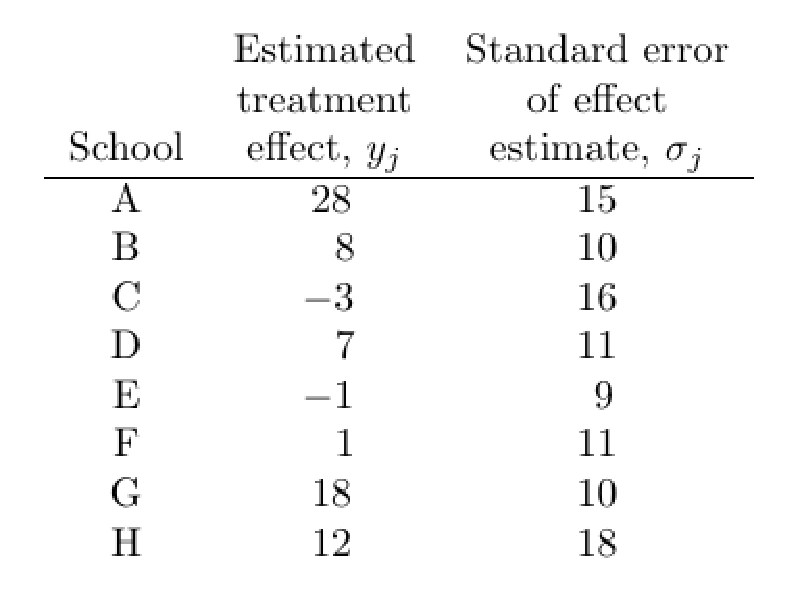
\includegraphics[scale = 0.45]{pictures/tbl_5_3.eps}
\caption{Pozorovaný efekt podpůrného programu}
\label{tbl_5_3}
\end{figure}
Implicitním předpokladem tohoto přístupu je, že všechny experimenty mají stejný efekt a data v tabulce na obrázku 5.7 tak lze považovat za osm pozorování z normálního rozdělení se známým rozptylem. Při použití neinformativního apriorního rozdělení je aposteriorní střední hodnota společného efektu programu na uvažovaných osmi školách $\overline{y}_{\cdot \cdot}$ dle (5.19) s tím, že $\overline{y}_{\cdot j}$ je nahrazeno $\overline{y}_j$. Takto získaný aposteriorní odhad je $\overline{y}_{\cdot \cdot} = 7.7$ s aposteriorním rozptylem $\sum_{j = 1}^8 \frac{1}{\sigma_j^2}^{-1} = 16.6$.\footnote{Při výpočtu rozptylu bylo využito skutečnosti, že jednotlivé experimenty jsou nezávislé.} Odpovídající 95\% aposteriorní interval spolehlivosti je tak $[-0.5, 15.9]$ nebo také $[8 \pm 8]$. Pro klasický test hypotézy o shodnosti jednotlivých $\theta_j$ je $\chi^2$ statistika menší než je počet stupňů volnosti, konkrétně $\sum_{j = 1}^8 \frac{(y_j - \overline{y}_{\cdot \cdot})}{\sigma_j^2} = 4.6$. Jinými slovy, $\hat{\tau}^2$ vypočtené dle (5.37) je záporné.

Otázkou nicméně zůstává, zda-li je výsledek dodatečných 28 bodů pro školu A v kontextu ostatních škol vůbec uvěřitelný. Předpokládejme, že tabulka na obrázku 5.7 představuje náhodné výběry z normálního rozdělení se střední hodnotou 8 bodů a směrodatnou odchylkou 13 bodů.\footnote{Směrodatná odchylka byla vypočtena jako odmocnina průměru rozptylů za uvažovaných osm škol.} Pak, na základě očekávaných hodnot normálních pořadových statistik, můžeme očekávat hodnoty 26, 19, 14, 10, 6, 2, -3 a -9 bodů, což je v souladu s hodnotami uvedenými v tabulce na obrázku 5.7.

\subsubsection{Problematika nezávislých a sdílených odhadů}

Uvažujme efekt ve škole A, tj. $\theta_1$, který je 28.4 dodatečných bodů se standardní směrodatnou odchylkou 14.9 za předpokladu nezávislých odhadů. To je v kontrastu se sdíleným odhadem, který má střední hodnotu 7.7 a směrodatnou odchylku 4.1. Nezávislé odhady implikují aposteriorní tvrzení \textit{`pravděpodobnost, že skutečný efekt v případě školy A je větší než 28.4 bodů, je 50\%'}, což je, s ohledem na výsledky ostatních škol, zpochybnitelné. Na druhou stranu, sdílený odhad implikuje tvrzení \textit{`pravděpodobnost, že skutečný efekt programu v případě školy A je menší než 7.7 bodů, je 50\%'}, což se zdá v být v příkrém rozporu s pozorovaných efektem 28 bodů. Další tvrzení, které společný odhad implikuje, je \textit{`pravděpodobnost, že skutečný efekt programu na škole A je menší než na škole B, je 50\%'}, což je opět poměrně těžké obhájit tváří v tvář tabulce na obrázku 5.7. Řešením je zkombinovat informaci ze všech osmi experimentů bez toho, aniž bychom předpokládali, že všechna $\theta_j$ jsou shodná, což nám umožňuje výše diskutovaný hierarchický model.

\subsection{Aposteriorní simulace v rámci hierarchického modelu}

Následně můžeme vypočíst aposteriorní rozdělení parametrů $\theta_1, ..., \theta_8$ založené na normálním modelu, který jsme představili v sekci 5.4. Nejprve náhodně vybereme hodnoty parametrů $\tau$, $\mu$ a $\theta$ z jejich aposteriorních rozdělení, přičemž předpokládáme, že (a) výběrové směrodatné odchylky $\sigma_j$ jsou dány hodnotami v tabulce na obrázku 5.7 a že (b) apriorní uniformní rozdělení pro parametry $\mu$ a $\tau$ jsou vzájemně nezávislá.

\subsection{Výsledky}

Marginální aposteriorní rozdělení $p(\tau|y)$ získané na základě (5.35) je zobrazeno na obrázku 5.8.
\begin{figure}[htp]
\centering
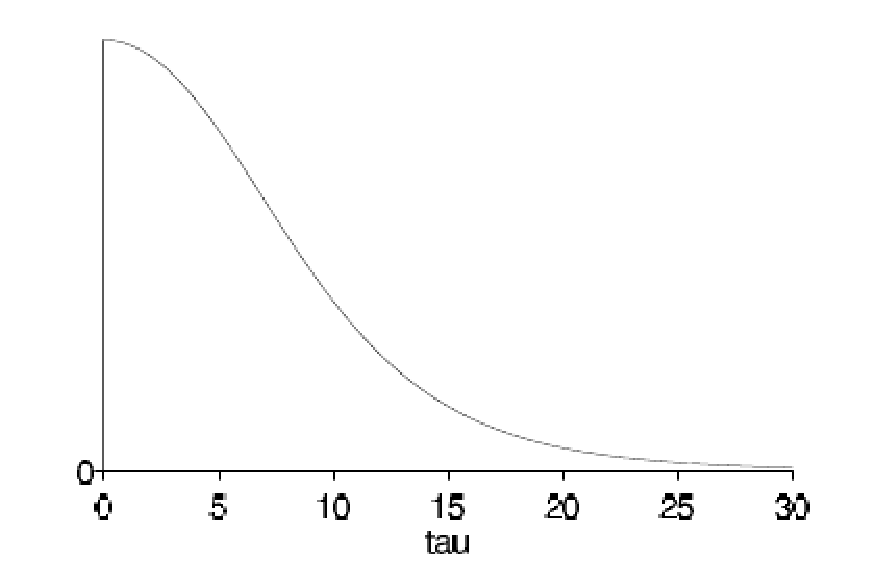
\includegraphics[scale = 0.45]{pictures/fig_5_5.eps}
\caption{Marginální aposteriorní rozdělení $p(\tau | y)$ pro standardní směrodatnou odchylku efektu speciálního programu na podporu studentů}
\label{fig_5_5}
\end{figure}
Hodnoty okolo nula bodů mají přiřazenu nejvyšší hustotu pravděpodobnosti; hodnoty vyšší než 25 bodů mají téměř nulovou hustotu pravděpodobnosti. Inference týkající se marginálního rozdělení ostatních parametrů a jejich sdružené rozdělení lze získat z nasimulovaných hodnot.

Podmíněné střední hodnoty $E(\theta_j|\tau, y)$ získané průměrováním přes $\mu$ jsou zobrazeny jako funkce $\tau$ na obrázku 5.8.
\begin{figure}[htp]
\centering
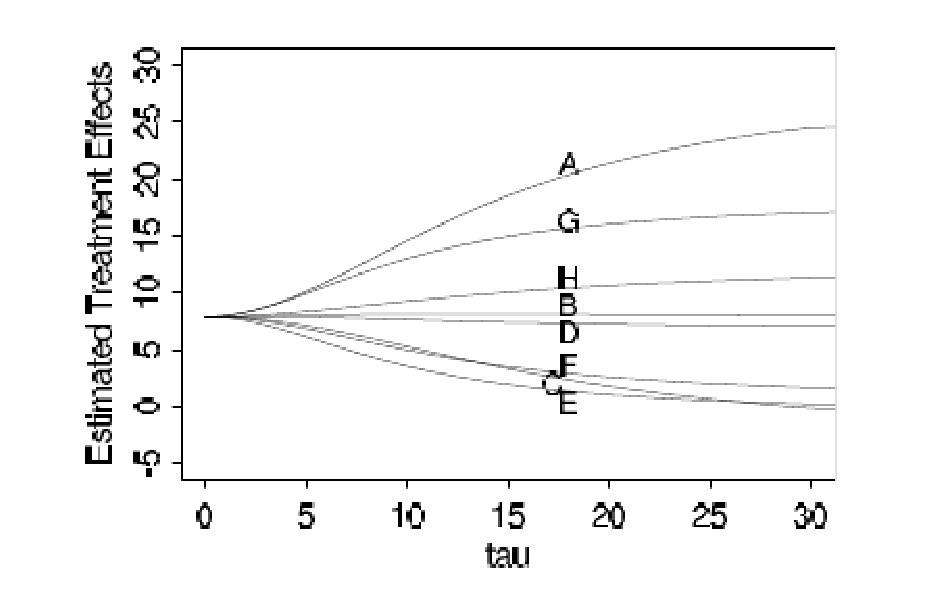
\includegraphics[scale = 0.45]{pictures/fig_5_6.eps}
\caption{Podmíněné aposteriorní střední hodnoty $E(\theta_j | \tau, y)$ efektu programu na podporu studentů jako funkce směrodatné odchylky $\tau$. Graf školy C protíná grafy škol E a F, protože C má vyšší směrodatnou odchylku a jeho odhad je tak vychýlen směrem k celkové střední hodnotě.}
\label{fig_5_6}
\end{figure}
Porovnáním obrázků 5.8 a 5.9, které mají shodné měřítko na vodorovné ose, vidíme, že pro většinu `pravděpodobných' hodnot  parametru $\tau$ jsou odhadnuté efekty relativně blízko u sebe. S tím, jak se $\tau$ stává větším, což odpovídá větším rozdílům mezi jednotlivými školami, se jednotlivé odhady blíží více a více hodnotám v tabulce na obrázku 5.7.

Grafy na obrázku 5.10 představují podmíněné směrodatné odchylky $sd(\theta_j | \tau, y)$ jako funkci $\tau$. S tím, jak se $\tau$ zvyšuje, zvyšuje se potenciální odlišnost dopadu programu na jednotlivé školy, což se projevuje nárůstem aposteriorní nejistoty jednotlivých $\theta_j$, která se blíží standardním směrodatným odchylkám v tabulce na obrázku 5.7 v limitě $\tau \rightarrow \infty$.
\begin{figure}[htp]
\centering
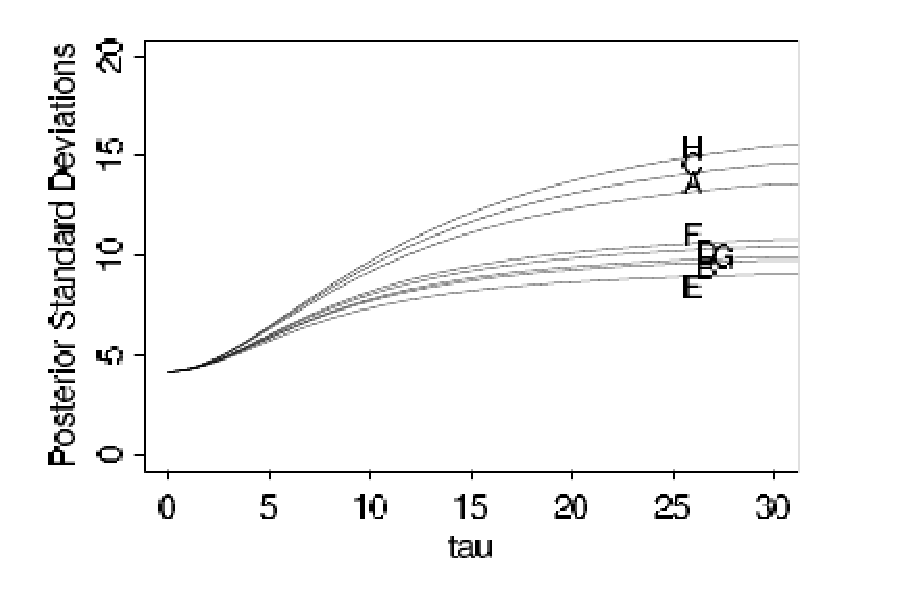
\includegraphics[scale = 0.45]{pictures/fig_5_7.eps}
\caption{Podmíněné aposteriorní směrodatné odchylky $sd(\theta_j | \tau, y)$ vlivu programu na podporu studentů jako funkce parametru $\tau$}
\label{fig_5_7}
\end{figure}

Na závěr bychom měli poznamenat, že pokud aplikujeme podmínění na aposteriorní mód parametru $\tau$, nezískáme přesnou sumární statistiku dat. Podmínění modální hodnotu (např. při odhadu metodou maximální věrohodnosti) hyperparametru jako je $\tau$ se často používá v praxi (alespoň jako aproximace), ačkoliv ignoruje nejistotu jeho aposteriorního rozdělení. Pro $\tau = 0$ je efekt programu pro všechny školy shodný, tj. předpokládáme střední hodnotu 7.7 bodů a směrodatnou odchylku 4.1 bodů. Obrázky 5.8 až 5.10 ilustrují, že tento stav předpokládá `konvergenci' odhadů pro všech osm škol. Tento problém je v našem ilustrativním příkladě obzvlášť akutní, protože se aposteriorní mód $\tau$ nachází na hranici parametrického prostoru. Sdružený aposteriorní modální odhad $(\theta_1, ..., \theta_J, \mu, \tau)$ pak `trpí' ještě většími problémy.

\subsection{Diskuse}

Tabulka na obrázku 5.11 sumarizuje 200 simulací pro uvažovaných osm škol. V jistém slova smyslu jsou tyto výsledky podobné společnému 95\% intervalu spolehlivosti $[8 \pm 8]$ a to v tom, že odpovídající Bayesiánské 95\% intervaly spolehlivosti se z velké části překrývají a jsou centrovány na mediánu v rozmezí 5 až 10 bodů. Na druhou stranu jsou tyto výsledky odlišné, protože naznačují různý efekt pro jednotlivé školy - 95\% Bayesiánské intervaly spolehlivosti jsou téměř dvakrát tak široké než interval spolehlivosti pro společný odhad s výrazně vyšší pravděpodobností 16 a více bodů (obzvláště v případě školy A) a větší pravděpodobnosti záporného efektu (obzvláště v případě školy C).

Pořadí škol v závislosti na efektu programu naznačené v tabulce na obrázku 5.11 je v podstatě totožné s pořadím, které bychom získali na základě osmi oddělených odhadů. Nicméně existují určité rozdíly v detailech - např. Bayesiánská pravděpodobnost, že efekt programu na škole A je vyšší než 28 bodů je méně než 10\%, což je významně méně než 50\% pravděpodobnost založená na samostatném odhadu pro tuto školu.
\begin{figure}[htp]
\centering
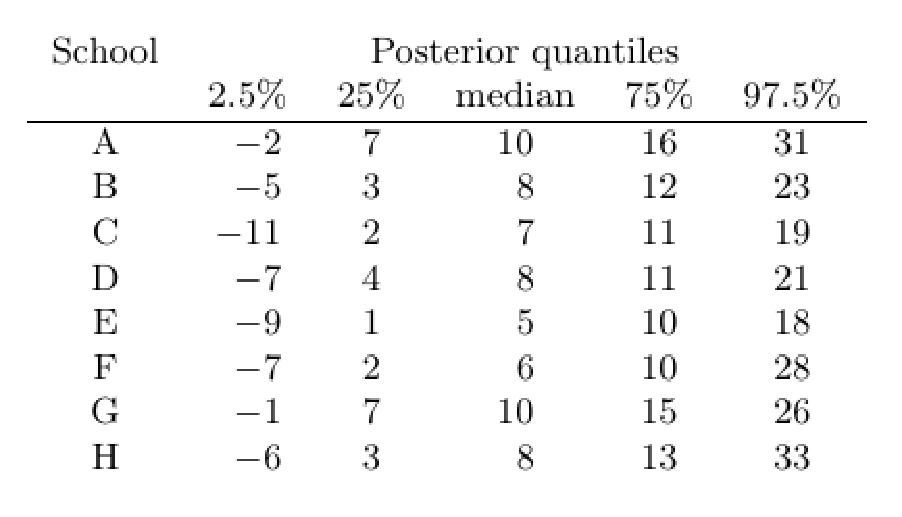
\includegraphics[scale = 0.45]{pictures/tbl_5_4.eps}
\caption{Sumarizace 200 simulací dopadu programu na osm uvažovaných škol}
\label{tbl_5_4}
\end{figure}

Obrázek 5.12a představuje histogram 200 simulací efektů pro školu A. Pokud máme k dispozici nasimulované hodnoty parametru $\theta$, můžeme klást i komplikovanější otázky jako např. jaké je aposteriorní rozdělení $max\{\theta_j\}$, kde $max\{\theta_j\}$ představuje efekt na nejúspěšnější z osmi škol. Obrázek 5.12b zobrazuje histogram 200 simulovaných efektů pro $max\{\theta_j\}$. Z obrázku vyplývá, že pouze 22 hodnot je vyšších než 28.4 bodů, a proto $Pr(max\{\theta_j\} > 28.4) \approx \frac{22}{200}$. Dalším příkladem je odhad $Pr(\theta_1 > \theta_3 | y)$, tj. aposteriorní pravděpodobnosti, že na škole A je program úspěšnější než na škole C, která je na základě nasimulovaných hodnot odhadnuta na $\frac{141}{200}$.
\begin{figure}[htp]
\centering
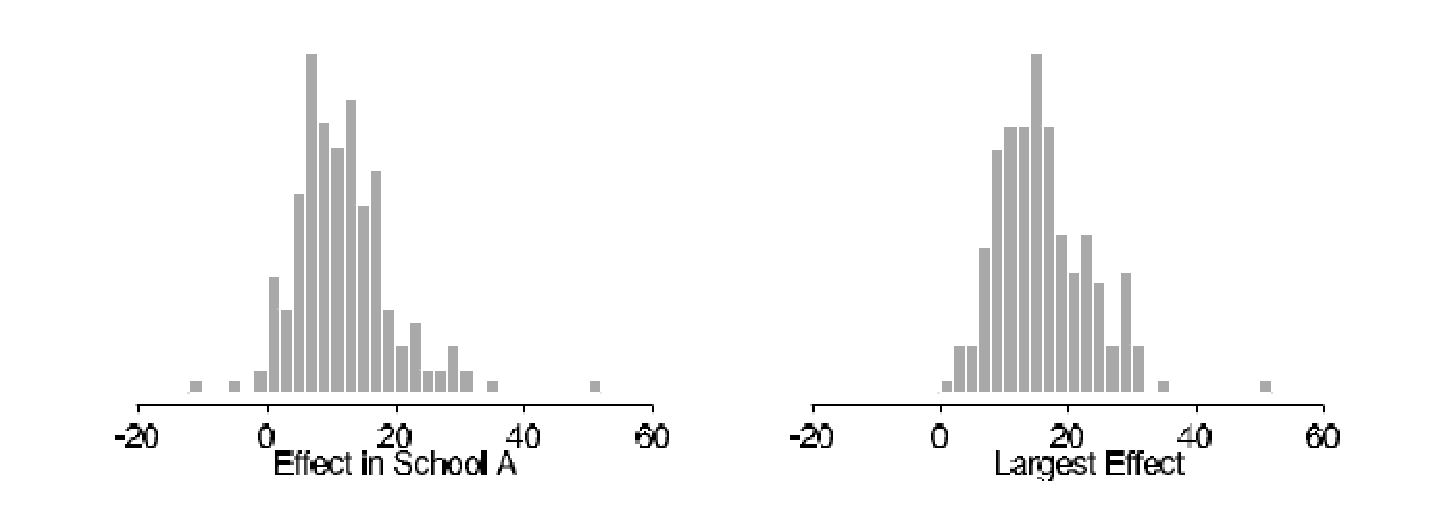
\includegraphics[scale = 0.45]{pictures/fig_5_8.eps}
\caption{Histogramy zkonstruované na základě 200 nasimulovaných hodnot - (a) histogram $\theta_1$, (b) histogram $max\{\theta_j\}$}
\label{fig_5_8}
\end{figure}

\section{Hierarchický model aplikovaný na meta analýzu}

Meta analýza je proces souhrnu závěrů výzkumných studií z určité oblasti výzkumu. Jako metoda kombinování informací z různých zdrojů je meta analýza blízká hierarchickému modelování. V následujícím textu se zaměříme na poměrně jednoduchou aplikaci hierarchického modelování na meta analýzu v medicíně.

Data pro náš příklad jsou uvedeny v tabulce na obrázku 5.13. Data se skládají ze dvou skupin pacientů postihnutých infarktem myokardu náhodně rozdělených do dvou skupin podle toho, zda-li jim byli aplikovány beta blokátory\footnote{Beta blokátory jsou skupina léků, která ovlivňuje centrální nervový systém a která pomáhá uvolňovat srdeční svaly.} Úmrtnost se pohybuje od 3\% do 21\% napříč studiemi, z nichž většina vykazuje mírný, byť statisticky nevýznamný, přínos beta blokátorů. Cílem meta analýzy je poskytnout kombinovanou analýzu studií s cílem získat indikovat celkovou sílu důkazů podporujících aplikaci beta blokátorů.
\begin{figure}[htp]
\centering
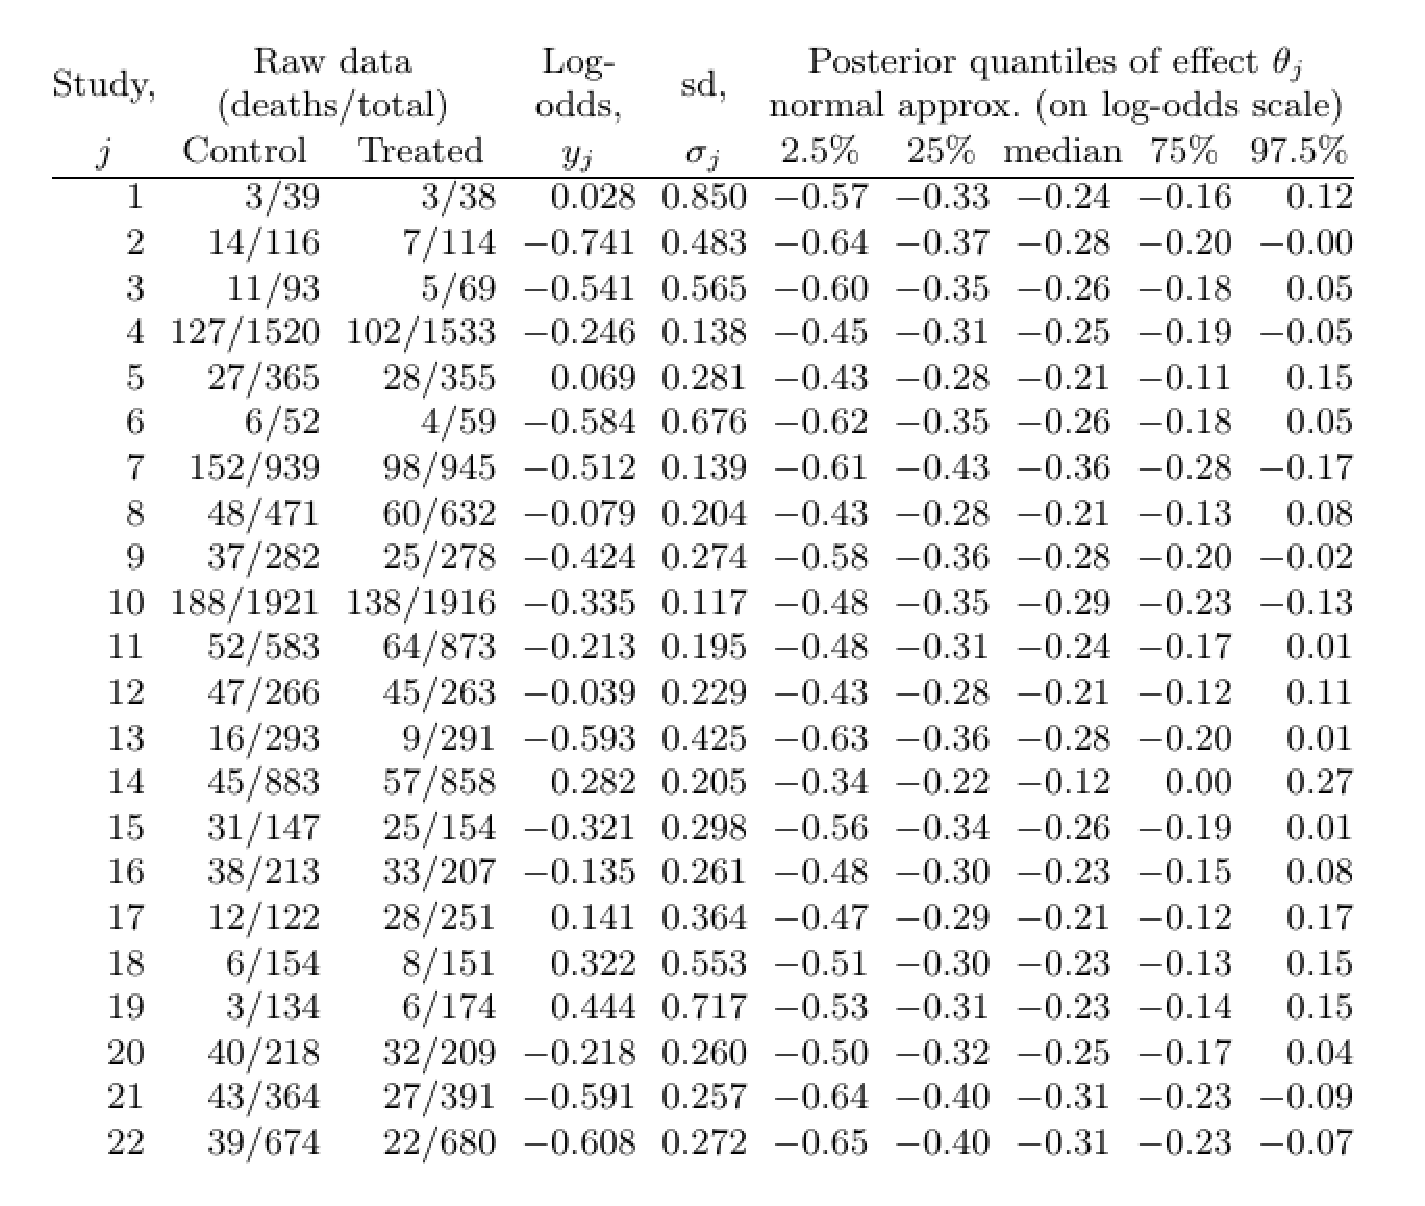
\includegraphics[scale = 0.45]{pictures/tbl_5_5.eps}
\caption{Výsledky 22 klinických testů tzv. beta blokátorů na snížení úmrtnosti po infarktu myokardu s empirickými log-odd hodnotami a přibližnými výběrovými rozptyly. Aposteriorní kvantily jsou založeny na 5~000 simulacích z Bayesiánského hierarchického modelu. Záporné efekty odpovídají snížené pravděpodobnosti úmrtí.}
\label{tbl_5_5}
\end{figure}

\subsection{Definování parametru}

Meta analýza zahrnuje data ve formě několika tabulek formátu 2x2. Jestliže $j$-tý klinický test zahrnuje $n_{0j}$ subjektů v kontrolní skupině (tj. ve skupině, které nebyl poskytnut lék) a $n_{1j}$ subjektů v testovací skupině (tj. ve skupině, které byl poskytnut lék) s počtem úmrtí $y_{0j}$ a $y_{1j}$ v první resp. ve druhé skupině, pak obvyklý model náhodného výběru zahrnuje dvě nezávislá binomická rozdělení s pravděpodobností úmrtí $p_{0j}$ a $p_{1j}$. Předmětem našeho zájmu jsou pak rozdíl pravděpodobností $p_{1j} - p_{0j}$, podíl pravděpodobností $p_{1j} / p_{0j}$ popř. podíl $\rho_j = \frac{p_{1j}}{1 - p_{1j}} / \frac{p_{0j}}{1 - p_{0j}}$. Z důvodu relativně snadné interpretace a skutečnosti, že se jeho aposteriorní rozdělení blíží normálnímu i v pro relativně malé výběry, se v následujícím textu zaměříme na logaritmus $\rho_j$, který budeme značit $\theta_j = \ln(\rho_j)$.

\subsection{Normální aproximace věrohodnostní funkce}

Jednoduchou Bayesiánskou analýzu můžeme založit na předpokladu normality, který jsme představili v předchozím textu, pokud závěry každého testu $j$ vyjádříme pomocí normální věrohodnostní funkce definované pro parametr $\theta_j$. Jeden z možných přístupů je založený na logit funkci, kdy $\theta_j$ můžeme odhadnout pomocí
\begin{equation}
y_j = \ln \Big(\frac{y_{1j}}{n_{1j} - y_{1j}}\Big) - \ln \Big(\frac{y_{0j}}{n_{0j} - y_{0j}}\Big)
\end{equation}
s výběrovým rozptylem
\begin{equation}
\sigma_j^2 = \frac{1}{y_{1j}} + \frac{1}{n_{1j} - y_{1j}} + \frac{1}{y_{0j}} + \frac{1}{n_{0j} - y_{0j}}.
\end{equation}

Odhadované hodnoty $y_j$ a jím odpovídající směrodatné odchylky $\sigma_j^2$ jsou zobrazeny jako čtvrtý a pátý sloupec tabulky na obrázku 5.13. V následujícím textu použijeme hierarchickou Bayesiánskou analýzu ke kombinaci výsledků 22 studií uvedených v této tabulce, čímž získáme lepší odhady jednotlivých parametrů $\theta_j$ společně s odhadem střední hodnoty a směrodatné odchylky přes všechny klinické testy.

\subsection{Inference v meta analýze}

Pomocí Bayesiánského přístupu se pokusíme zjistit, zda-li je možné považovat všechny studie za vzájemně porovnatelné v tom smyslu, že můžeme všechny jedince v těchto studiích považovat za náhodně vybrané z téže populace. V opačném případě nelze z výsledků jedné studie uvažovat na možné výsledky ostatních studií. Další možností je, že jednotlivé studie je možné považovat za vzájemně zaměnitelné, avšak nikoliv nezbytně nutně za identické popř. vzájemně nesouvisející. Jinými slovy, mezi jednotlivými testy existují rozdíly, nicméně tyto rozdíly nemají předvídatelný efekt. Tato poslední verze tak představuje kompromis mezi dvěma předchozími přístupy.

\subsection{Hierarchický normální model}

Nechť $y_j$ představuje bodové odhady $\theta_j$ získané na základě (5.38), kde $j = 1, ..., J$. Hierarchický normální model předpokládá
\begin{equation}
y_j | \theta_j, \sigma_j \sim N(\theta_j, \sigma_j^2),
\end{equation}
kde $\sigma_j$ je odpovídající směrodatná odchylka vypočtená pomocí (5.39), o které předpokládáme, že ji známe a že není zatížená chybou. Toto zjednodušení ve smyslu známé směrodatné odchylky má jen malý vliv, protože pro velké výběry (téměř všechny studie mají více než 50 pacientů jak v kontrolní tak testovací skupině) jsou binominální rozptyly poměrně přesně odhadnuty.

Nejprve s využitím předpokladu zaměnitelnosti použijeme normální apriorní rozdělení se střední hodnotu $\mu$ a směrodatnou odchylkou $\tau$, což jsou neznámé hyperparametry. K tomu budeme potřebovat hyperapriorní rozdělení pro $\mu$ a $\tau$. Pro hyperparametr $\mu$ je možné použít lokálně uniformní apriorní rozdělení, protože i v případě relativně malého počtu studií budou kombinovaná data dostatečně informativní ohledně populační střední hodnoty. Také v případě hyperparametru $\tau$ je nejjednodušší variantou aplikace lokálně uniformního rozdělení.

\subsection{Výsledky analýzy a porovnání s jednoduššími metodami}

Pokud bychom zkonstruovali graf, který je analogií grafu na obrázku 5.8, zjistili bychom, že marginální aposteriorní rozdělení hyperparametru $\tau$ dosahuje maxima pro nenulové hodnoty, ačkoliv hodnoty blízké nule jsou poměrně pravděpodobné s tím, že $\tau = 0$ má hustotu pravděpodobnosti pouze o 25\% menší než v modální hodnotě. Aposteriorní kvantily parametrů $\theta_j$ na logit měřítku pro uvažovaných 22 studií jsou uvedeny v posledních sloupcích tabulky na obrázku 5.13.

Protože je aposteriorní rozdělení parametru $\tau$ koncentrováno kolem hodnot, které jsou v porovnání s výběrovými směrodatnými odchylkami poměrně malé\footnote{To je patrné, pokud porovnáme hodnotu mediánu $\tau$ z tabulky na obrázku 5.14 s hodnotami $\sigma_j$ na obrázku 5.13.}, jsou Bayesiánské odhady zredukované a to zejména v případě testů s nízkou interní přesností.\footnote{Jedná se např. o testy 1, 6 a 18.} Významná homogenita klinických testů je dále indikována významným poklesem aposteriorního rozptylu při přechodu z odhadů pro jednotlivé testy na Bayesiánské odhady, které využívají data ze všech klinických testů. Pokud bychom použili přibližný postup pro odhad $\tau$, pak bychom získali směrodatnou odchylku, která by byla významně nižší než odpovídající Bayesiánský odhad.
\begin{figure}[htp]
\centering
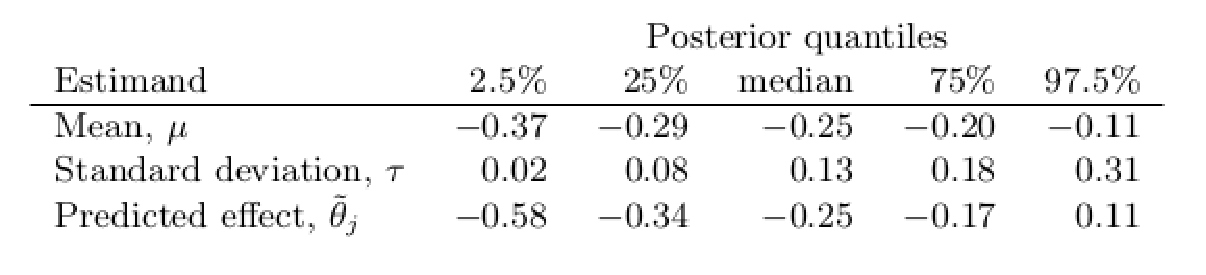
\includegraphics[scale = 0.45]{pictures/tbl_5_6.eps}
\caption{Vybrané kvantily pro střední hodnotu, směrodatnou odchylku a predikovaný parametr $\tilde{\theta}_j$ pro hypotetickou budoucí studii. Souhrnné statistiky jsou odvozeny z údajů v tabulce na obrázku 5.13 pro klinické testy beta blokátoru. Parametry $\tilde{\theta}_j$ předpokládají log-odd transformaci.}
\label{tbl_5_6}
\end{figure}

Pokud bychom zkonstruovali histogramy simulovaných aposteriorních hustot pravděpodobnosti jednotlivých $\theta_j$, byly by tyto histogramy výrazně sešikmené, ačkoliv rozdělení celkové střední hodnoty je symetrické. Aposteriorní rozdělení parametru $\theta_j$ pro nepřesné studie (např. 2 a 18) vykazují v porovnání s přesnějšími studiemi (např. 7 a 14) dlouhé chvosty.

V meta analýze se často soustředíme na odhad celkové střední hodnoty $\mu$. Pokud bychom vzájemně překryli grafy podmíněné aposteriorní střední hodnoty a směrodatné odchylky parametru $\mu$ pro dané $\tau$ s grafem aposteriorního rozdělení parametru $\tau$, zjistili bychom, že (a) rozumné rozmezí hodnot $E(\mu | \tau, y)$ je poměrně úzké a to zhruba od -0.26 do -0.24, nicméně (b) interval $sd(u | \tau, y)$ je nejméně o dvakrát tak delší než interval rozumných hodnot $\tau$. To ilustruje důležitost průměrování přes $\tau$ s cílem vzít v potaz nejistotu odhadu tohoto hyperparametru.\footnote{Např. podmíněná aposteriorní směrodatná odchylka $sd(\mu | \tau, y)$ má hodnotu 0.060 pro $\tau = 0.13$, nicméně po zprůměrování přes $\tau$ získáme hodnotu $sd(\mu|y) = 0.071$.}

Tabulka na obrázku 5.14 je souhrnem aposteriorních inferencí pro hyperparametry $\mu$ a $\tau$ a predikovaného efektu $\tilde{\theta}_j$ pro hypotetické budoucí klinické studie. Přibližný 95\% interval spolehlivosti parametru $\mu$ je $[-0.37, -0.11]$ resp. $[0.69, 0.90]$ po převedení na odd-log škálu (tj. po aplikaci exponenciály). Naproti tomu 95\% interval spolehlivosti, který je výsledkem společného odhadu\footnote{Společný odhad je odhad založený na všech klinických testech, jejichž všechna data dáme na `jednu hromadu', čímž předpokládáme $\tau = 0$.}, je významně užší a to $[0.70, 0.85]$. Nejistotu ohledně pravděpodobného efektu podání beta blokátorů můžeme prezentovat formou efektu $\tilde{\theta}_J$ nové hypotetické klinické studie, kterou můžeme považovat za zaměnitelnou s již realizovanými klinickými studiemi. Příslušná inference, která je zatížená ještě větší mírou nejistoty než tomu bylo v případě parametru $\mu$, je zachycena na posledním řádku tabulky na obrázku 5.14.

\section{Slabě informativní apriorní rozdělení hierarchických parametrů rozptylu}

Klíčovým prvkem výše uvedené analýzy je apriorní rozdělení hyperparametru $\tau$. Jako apriorní jsme použili uniformní rozdělení, nicméně literatura na Bayesiánskou statistiku nabízí řadu dalších neinformativních alternativ. Bohužel platí, že volba neinformativního apriorního rozdělení může mít zásadní vliv na výsledné inference a to zejména v případech, kdy je počet skupin $J$ malý stejně jako meziskupinový rozptyl $\tau$.

\subsection{Volba apriorního rozdělení}

\subsubsection{Nevlastní limita apriorního rozdělení}

Pro rozptyl na úrovni skupiny se jako nevlastní rozdělení často používají (a) uniformní rozdělení na intervalu $(0, A)$ pro $\tau$ nebo (b) inverzní gamma rozdělení s parametry $(\epsilon, \epsilon)$ pro $\tau^2$.

Uniformní rozdělení vede pro $A \rightarrow \infty$ k vlastnímu aposteriornímu rozdělení pokud $J \ge 3$. Proto pro konečné ale dostatečně vysoké $A$ nejsou inference příliš citlivé na konkrétní volbu jeho hodnoty.

Naproti tomu inverzní gamma rozdělení nevede k vlastnímu aposteriornímu rozdělení. To má za následek, že aposteriorní inference jsou citlivé na volbu $\epsilon$.

\subsubsection{Kalibrace}

Aposteriorní inference mohou být hodnoceny pomocí kalibrace aposteriorní střední hodnoty, což je Bayesiánská analogie pojmu `zkreslení' v klasické statistice. Pokud aposteriorní střední hodnotu označíme jako $\hat{\theta} = E(\theta | y)$, můžeme chybu v kalibraci aposteriorní střední hodnoty definovat jako $E(\theta | \hat{\theta}) - \hat{\theta}$. Pokud je volba apriorního rozdělení správná - tj. pokud jsou data získána tak, že nejprve náhodně vybereme $\theta$ z $p(\theta)$ a následně náhodně vybereme $y$ z $p(y | \theta)$ - pak je míra chyby v kalibraci nulová pro všechny hodnoty $\hat{\theta}$.

Jinými slovy, v klasické statistice při analýze zkreslení podmiňujeme skutečným $\theta$ a zkoumáme jeho odhad $\hat{\theta}$ založený na datech. Naproti tomu v Bayesiánském přístupu podmiňujme pozorovanými daty $y$ (a tím pádem také odhadem $\hat{\theta}$) a zkoumáme rozdělení parametru $\theta$, které mohlo vést k pozorovaným datům.

V případě nevlastních modelů však není možné náhodně vybrat $\theta$ z nenormalizovaného rozdělení. Abychom mohli zhodnotit kalibraci, je třeba předpokládat `skutečné apriorní rozdělení', z kterého bychom mohli náhodně vybrat $\theta$, společně `inferenčním apriorním rozdělením', které je použito v případě Bayesiánské inference.

V případě hierarchického modelu pro osm škol z výše uvedeného ilustračního příkladu, můžeme uvažovat nevlastní uniformní rozdělení pro $\tau$ jako limitní apriorní uniformní rozdělení nad intervalem $(0, A)$, kde $A \rightarrow \infty$. Pro libovolnou konečnou hodnotu $A$ vede nevlastní uniformní rozdělení k inferencím z pozitivním zkreslením, tj. nadhodnocením (v průměru) $\tau$.

Demonstrujme toto zkreslení v následujících dvou krocích. Nejprve předpokládejme, že jak skutečné tak inferenční apriorní rozdělení pro $\tau$ jsou uniformní nad $(0, A)$. Je zřejmé, že v tomto případě je zkreslení nulové. Následně předpokládejme, že skutečné apriorní rozdělení je stále definované nad intervalem $(0, A)$, zatímco inferenční apriorní rozdělení je nově definované nad intervalem $(0, \infty)$. Změna intervalu uniformního rozdělení nutně vede k nárůstu $\hat{\theta}$ pro libovolná data $y$ bez toho, aby se změnilo skutečné $\theta$.

\subsection{Třídy neinformativní a slabě informativních apriorních rozdělení pro parametry rozptylu v hierarchickém modelu}

\subsection{Obecné předpoklady}

Neinformativní popř. slabě informativní apriorní rozdělení chápeme jako prozatímní. po té, co je model nakalibrován, je třeba zhodnotit, zda-li je výsledné aposteriorní rozdělení smysluplné. Pokud tomu tak není, že třeba zvolit alternativní apriorní rozdělení.

\subsubsection{Apriorní uniformní rozdělení}

Nejprve se zaměřme na apriorní uniformní rozdělení. V případě tohoto rozdělení musíme specifikovat interval, nad kterým je rozdělení definováno. Vzhledem k tomu, že $\tau > 0$, by se jako přirozená volba mohlo zdát použití uniformního rozdělení pro $\ln(\tau)$, což by však vedlo k nevlastnímu aposteriornímu rozdělení. Alternativou by mohlo být definovat apriorní rozdělení na omezeném intervalu $[-A, A]$ pro velké $A$, nicméně výsledné aposteriorní rozdělení by bylo silně závislé na volbě dolní hranice $-A$.

Důvodem problému je skutečnost, že marginální věrohodnostní funkce $p(y|\tau)$ - po integraci přes $\theta$ a $\mu$ v (5.23) - se pro $\tau \rightarrow 0$ blíží konečné nenulové hodnotě. Proto, pokud použijeme pro $\ln(\tau)$ apriorní uniformní rozdělení, bude mít aposteriorní rozdělení nekonečný integrál. Jinými slovy, v hierarchickém modelu nemohou data nikdy vyloučit nulový rozptyl na úrovni skupiny, a proto apriorní rozdělení nemůže vykazovat nekonečnou pravděpodobnostní masu v této oblasti.

Další možností je aplikace normální rozdělení přímo na parametr $\tau$. Toto rozdělení má konečný integrál blízko $\tau = 0$, čímž se vyhneme výše uvedenému problému. Nicméně daní je pozitivní zkreslení z důvodu nekonečné pravděpodobnostní masy pro $\tau \rightarrow \infty$. Pro $J < 3$, kde $J$ představuje počet skupin, tak získáváme nevlastní aposteriorní rozdělení, čímž vlastně tvrdíme, že $\tau = \infty$. Ve své podstatě je to logický závěr, protože na základě omezeného počtu skupin je obtížné usuzovat na jejich podobnost či rozdílnost a tím pádem rozhodnout, zda-li tyto skupiny máme pro účely inferencí sloučit či nikoliv. Nicméně v případě Bayesiánského přístupu je poněkud krkolomné toto rozhodnutí učinit dopředu v situaci, kdy nám data neposkytují dostatečnou informaci. Dále, pro relativně malá $J$, jako např. 4 nebo 5, bychom měli mít na paměti, že tlustý pravý chvost aposteriorního rozdělení může vést k nadhodnocení $\tau$, a tím pádem vést k sloučení skupin, což nemusí být v porovnání s odhadem jednotlivých $\theta_j$ optimální.

Tyto nevlastní apriorní uniformní rozdělení můžeme interpretovat jako limity slabě informativních podmíněných konjugátních apriorních rozdělení. Apriorní uniformní rozdělení pro $\ln(\tau)$ je ekvivalentní $p(\tau) \varpropto \tau^{-1}$ nebo $p(\tau^2) \varpropto \tau^{-2}$, které mají formu inverzního $\chi^2$ rozdělení s nula stupni volnosti a lze je chápat limitu vlastního inverzního apriorního gamma rozdělení.

Uniformní rozdělení pro $\tau$ je ekvivalentní k $p(\tau^2) \varpropto \tau^{-1}$, což je inverzní $\chi^2$ rozdělení s -1 stupni volnosti. Toto rozdělení sice nelze chápat jako limitu vlastního inverzního $\chi^2$ rozdělení (protože to musí mít kladný počet stupňů volnosti), ale lze ho chápat jako limitu rodiny $t$ rozdělení omezenou na kladný interval.

Další neinformativní apriorní rozdělení, které je někdy zmiňováno v Bayesiánské literatuře, je uniformní rozdělení pro $\tau^2$. Toto rozdělení však nedoporučujeme, protože trpí nadhodnocováním odhadovaných parametrů a navíc vyžaduje $J \ge 4$ skupin pro vlastní aposteriorní rozdělení.

\subsubsection{Inverzní apriorní gamma rozdělení}

Parametr $\tau$ v modelu (5.35) nelze popsat žádnou jednoduchou rodinou konjugátního apriorního rozdělení, protože jeho marginální věrohodnostní funkce je komplexní funkcí dat všech $J$ skupin. Nicméně rodina inverzního gamma rozdělení je podmíněně konjugátní za předpokladu, že známe ostatní parametry modelu. To znamená, že pokud $\tau^2$ sleduje inverzní apriorní gamma rozdělení, pak podmíněné aposteriorní rozdělení $p(\tau^2 | \theta, \mu, y)$ je také inverzní gamma rozdělení. Inverzní gamma rozdělení s parametry $(\alpha, \beta)$ pro parametr $\tau^2$ může být také vyjádřeno jako inverzní $\chi^2$ rozdělení se škálou $s^2 = \frac{\beta}{\alpha}$ a $\nu = 2 \alpha$ stupni volnosti. Parametrizace inverzního $\chi^2$ rozdělení pak může být užitečná pro porozumění informace, která je na pozadí volby konkrétního vlastního apriorního rozdělení.

Inverzní apriorní gamma rozdělení s parametry $(\epsilon, \epsilon)$ je pokusem o neinformativnost v rámci podmíněné konjugátní rodiny s nízkou hodnotou parametru $\epsilon$ jako např. 0.01 nebo 0.001. Problém tohoto apriorního rozdělení spočívá v tom, že $\epsilon \rightarrow 0$ implikuje nevlastní aposteriorní rozdělení. Proto musíme pro $\epsilon$ zvolit rozumnou kompromisní hodnotu. Bohužel odhady nad daty, pro které je možné aplikovat nízké hodnoty $\epsilon$, jsou velmi citlivé na volbu konkrétní hodnoty tohoto parametru a výsledné apriorní rozdělení, jak je ilustrováno na obrázku 5.15 lze stěží považovat za neinformativní.
\begin{figure}[htp]
\centering
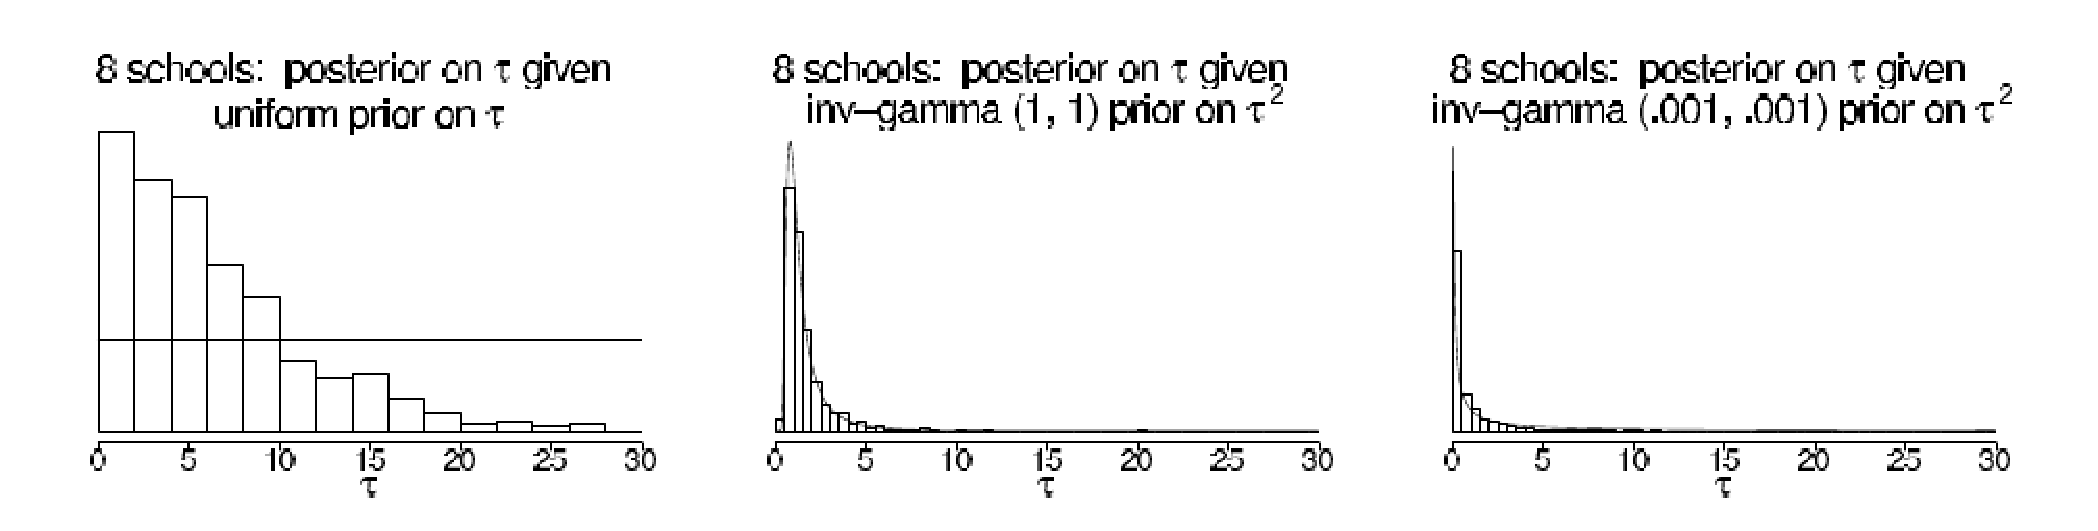
\includegraphics[scale = 0.42]{pictures/fig_5_9.eps}
\caption{Histogramy aposteriorních simulací parametru $\tau$ založených na třech apriorních rozděleních: (a) apriorním uniformním rozdělení pro $\tau$, (b) inverzním apriorním gamma rozdělením s parametry $(1, 1)$ pro $\tau^2$ a (c) inverzním apriorním gamma rozdělením s parametry $(0.001, 0.001)$ pro $\tau^2$. Souvislá čára na každém z grafů značí odpovídající apriorní rozdělení parametru $\tau$. Pro modely (b) a (c) je rozdělení parametru $\tau$ vypočteno s pomocí gamma rozdělení vynásobeného Jacobiánem transformace $1/\tau^2$. Jak je patrné z grafů, jsou aposteriorní inference v těchto modelech silně svázány s apriorním rozdělením.}
\label{fig_5_9}
\end{figure}

\subsubsection{Poloviční apriorní Cauchyho rozdělení}

Kromě výše uvedených, bychom také měli zvážit použití rodiny $t$ rozdělení\footnote{Vzhledem k podmínce $\tau > 0$ nás zajímá pouze část $t$ rozdělení definovaná nad intervalem $(0, \infty)$.} jako alternativní třídu, která jako mezní případy zahrnuje normální a Cauchyho rozdělení. Nejprve pro parametr $\tau$ použijeme $t$ rozdělení, protože jej lze s pomocí změny definice parametrů vyjádřit jako podmíněné konjugátní apriorní rozdělení.

Pro naše účely si postačí uvědomit, že poloviční Cauchyho rozdělení může být příhodné slabě informativní rozdělení - toto rozdělení má poměrně `široké' maximum a jediný škálový parametr, který budeme značit $A$, a který je zpravidla nastaven na vysokou hodnotu. V limitním případě $A \rightarrow \infty$  přechází Cauchyho rozdělení do uniformního rozdělení. Vysoké nicméně konečné hodnoty $A$ pak představují rozdělení, které lze považovat za slabě informativní, protože mají i ve chvostě mírný sklon (na rozdíl od např. polovičního normálního rozdělení) a umožňují tak dominanci dat, pokud je v tomto regionu věrohodnostní funkce silná. Poloviční Cauchyho rozdělení budeme používat v případech, kdy je parametr rozptylu odhadován na základě malého počtu skupin, tj. v případech, kdy jsou inference citlivé na volbu slabě informativního apriorního rozdělení.

\subsection{Aplikace na ilustrativní příklad osmi škol}

Vraťme se k našemu ilustrativnímu příkladu. Připomeňme, že parametry $\theta_1, ..., \theta_8$ představují relativní efekt programu na podporu studentů, který byl představen na osmi školách, a že parametr $\tau$ představuje směrodatnou odchylku tohoto efektu mezi jednotlivými školami. Efekt programu je měřen jako počet bodů, které studenti získali v testu jehož bodové rozpětí je 200 až 800 bodů s průměrným skóre 500 bodů. Největší možné rozpětí zkoumaného efektu je tak 300 bodů s realistickou směrodatnou odchylkou přibližně 100 bodů.

\subsubsection{Neinformativní apriorní rozdělení}

Obrázek 5.15 představuje aposteriorní rozdělení pro 8 škol, které jsou výsledkem tří různých voleb apriorních neinformativních rozdělení.


První z grafů na obrázku představuje aposteriorní rozdělení parametru $\tau$ pro uniformní apriorní rozdělení. Data poskytují oporu pro hodnoty $0 < \tau < 20$ s tenkým chvostem pro $\tau > 20$. Naproti tomu prostřední graf je založen na inverzním apriorní gamma rozdělení s parametry $(1, 1)$ pro $\tau^2$. Z aposteriorního rozdělení je zřejmé, že aposteriorní střední hodnota a medián parametru $\tau$ jsou menší a pravděpodobnostní masa je více koncentrována v levé části grafu, než tomu bylo v předchozím případě. Poslední z trojice grafů pak odpovídá inverznímu apriornímu gamma rozdělení s parametry $(0.001, 0.001)$ pro $\tau^2$. V tomto případě je celá pravděpodobnostní masa ještě více `natlačena' směrem k nižším hodnotám $\tau$, což je dáno tím, že marginální věrohodnostní funkce parametru $\tau$ zůstává i v blízkosti bodu 0 vysoká. Ze všech tří uvažovaných apriorních rozdělení se tedy zdá být nejvhodnější nejjednodušší přístup založení na apriorním uniformním rozdělení.

\subsection{Slabě informativní apriorní rozdělení}

Uniformní rozdělení je vhodné pro situaci, kdy analyzujeme osm škol, Nicméně v případě, kdy počet škol $J$ menší, poskytují data pouze omezenou informaci o mezi skupinovém rozptylu. Neinformativní apriorní rozdělení pak může mít za následek aposteriorní rozdělení, které je nevlastní nebo sice vlastní, nicméně nerealisticky `široké'. Pro ilustraci tohoto problému použijeme data pouze prvních tří škol.

\begin{figure}[htp]
\centering
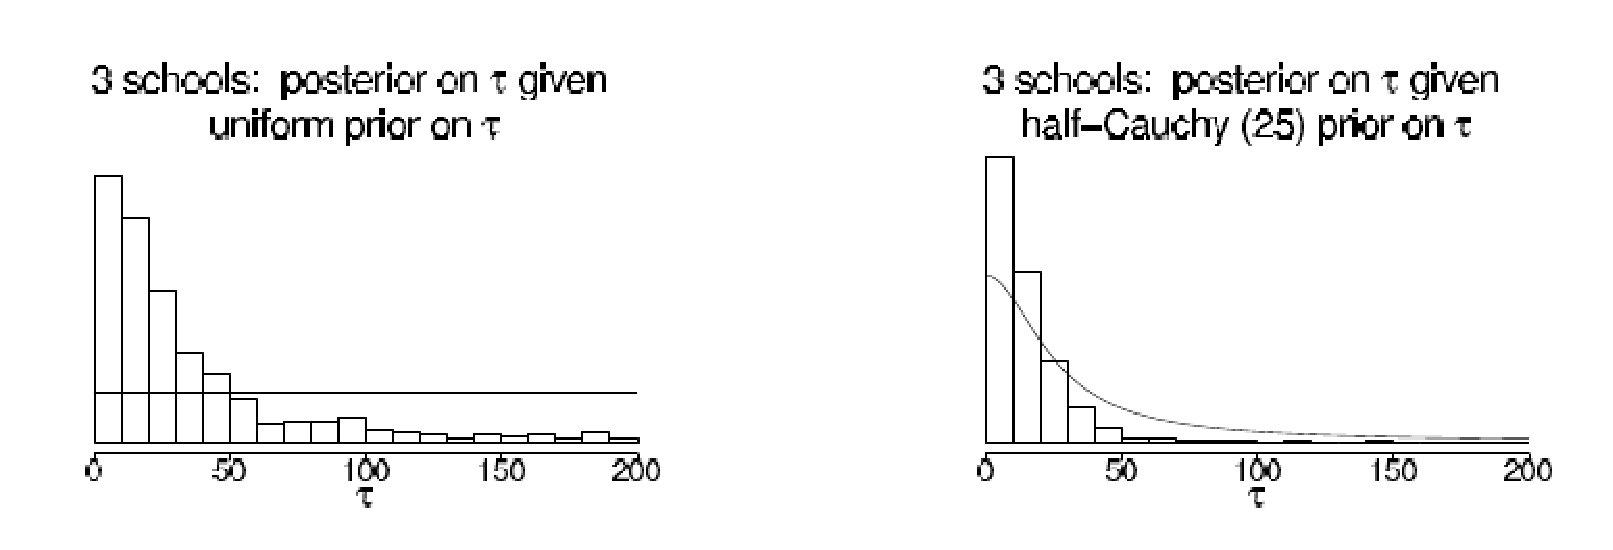
\includegraphics[scale = 0.42]{pictures/fig_5_10.eps}
\caption{Histogramy aposteriorních simulací parametru $\tau$ na datech tří škol založených na dvou apriorních rozdělení: (a) apriorním uniformním rozdělení na intervalu $(0, \infty)$ a (b) polovičního Cauchyho rozdělení s parametrem 25, které plní roli slabě informativního rozdělení kdy předpokládáme, že skutečná hodnota $\tau$ se nachází významně pod 100 body. Souvislá čára na každém z grafů značí odpovídající apriorní rozdělení parametru $\tau$. S pouze $J = 3$ skupinami je neinformativní apriorní uniformní rozdělení příliš `slabé'. Naproti tomu vlastní Cauchyho rozdělení se zdá být lepší variantou, protože nedeformuje inference v regionu s vysokými hodnotami věrohodnostní funkce.}
\label{fig_5_10}
\end{figure}

Obrázek 5.16 ilustruje aposteriorní rozdělení parametru $\tau$ pro dvě rozdílná aposteriorní rozdělení. Prvním je uniformní rozdělení, které se osvědčilo v případě $J = 8$ škol. Nicméně pro $J = 3$ škol má výsledné aposteriorní rozdělení příliš dlouhý pravý chvost, který obsahuje hodnoty $\tau$ příliš vysoké na to, aby byly realistické. Pravý histogram na obrázku 5.16 pak zobrazuje aposteriorní rozdělení parametru $\tau$ založené na polovičním apriorním Cauchyho rozdělení s parametrem $A = 25$.\footnote{Hodnotu parametru $A$ jsme záměrně zvolili vyšší než bychom očekávali pro směrodatnou odchylku podkladových $\theta_j$ v kontextu našeho ilustrativního příkladu. Důvodem je, že takto zvolený model limituje parametr $\tau$ pouze velmi omezeně.} Aposteriorního rozdělení, které je v grafu znázorněné souvislou čárou, dosahuje vysokých hodnot nad intervalem $\tau < 50$, který představuje nejrealističtější hodnoty parametru $\tau$. Z tohoto důvodu se poloviční Cauchyho rozdělení zdá být v roli apriorního rozdělení vhodnější než často používané normální rozdělení.

Poloviční Cauchyho rozdělení je možné použít také v případě, kdy bychom vzorek rozšířili na původních $J = 8$ škol. V tomto případě se však s ohledem na jeho jednoduchost jako vhodnější jeví normální rozdělení.
\chapter{Slovník}

\begin{table}
\begin{center}
\begin{tabular}{l l} 
\bf{anglicky} & \bf{česky}\\
\hline
time series & časová řada\\
cross-sectional data & průřezová data\\
pooled cross section data & sdružená průřezová data\\
panel data & panelová data\\
regression model & regresní model\\
explanatory variable & vysvětlující veličina\\
independent variable & nezávislá veličina\\
dependent variable & závislá veličina\\
error term / disturbance & chybová složka / chyba\\
slope parameter & parametr sklonu\\
intercept parameter & parametr průsečíku\\
population regression function (PRF) & populační regresní funkce\\
ordinary least square (OLS) estimates & odhad nejmenších čtverců\\
OLS regression line & OLS regresní přímka\\
sample regression function (SRF) & výběrová regresní funkce\\
residual & reziduum\\
sum of squared residuals & součet čtverců reziduí\\
total sum of squares (SST) & celkový součet čtverců\\
explained sum of squares (SSE) & vysvětlený součet čtverců\\
residual sum of squares (SSR) & reziduální součet čtverců\\
goodnes of fit & míra shody\\
unbiasedness of OLS & nestrannost OLS odhadů\\
standard error of regression (SER) & standardní směrodatná odchylka regrese\\
omitted variable bias & zkreslení z titulu opomenutí\\
 & relevantní vysvětlující proměnné\\
variance inflation factor (VIF) & inflační faktor rozptylu\\
degrees of freedom & stupně volnosti\\
standard deviation & směrodatná odchylka\\
standard error & směrodatná chyba\\
best linear unbiased estimator (BLUE) & nejlepší nezkreslený lineární odhad\\
sampling distribution & výběrové rozdělení\\
classical liner model (CLM) assumptions & předpoklady klasického lineárního modelu\\
one-sided test & jednostranný test\\
two-sided test & dvoustranný test\\
significance level & hladina významnosti\\
p-value & p-hodnota\\
confidence interval & interval spolehlivosti\\
multiple (joint) hypothesis & vícenásobná (sdružená) hypotéza\\
unrestricted model & neomezený model\\
restricted model & omezený model\\
adjusted $R^2$ & korigované $R^2$\\
resampling method & metoda opakovaného výběru\\
binary (dummy) variable & binární veličina\\
dummy variable trap & past binární veličiny\\
linear probability model (LPM) & lineární pravděpodobnostní model\\
generalized least squares (GLS) estimators & obecné odhady metodou nejmenších čtverců\\
weighted least squares (WLS) estimators & odhady metodou vážených nejmenších čtverců\\
\end{tabular}
\caption{Anglicko-český slovník vybraných statistických pojmů}
\end{center}
\end{table}

\begin{table}
\begin{center}
\begin{tabular}{l l} 
\bf{anglicky} & \bf{česky}\\
\hline
finite distributed lag (FDL) model & model s konečným rozdělením zpoždění\\
impact propensity & propensitní účinek\\
long-run propensity & dlouhodobá propensita\\
comtemporaneous exogenous & souběžně exogenní\\
serial correlation aka autocorrelation & sériová korelace aka autokorelace\\
spurious correlation & zdánlivá korelace\\
stationary time series & stacionární časové řada\\
weakly dependent time series & slabě závislá časová řada\\
covariance stationary proces & kovariančně stacionární proces\\
independent identically distributed (iid) & nezávislé stejnoměrně rozdělené\\
 & (náhodné veličiny)\\
moving average process of order one [MA(1)] & proces klouzavého průměru řádu jedna\\
autoregressive process of order one [AR(1)] & autoregresivní proces řádu jedna\\
trend-stacionary process & trendově stacionární proces\\
law of iterated expectations & zákon iterované střední hodnoty\\
unit root process & proces s jednotkovým kořenem\\
integrated process of order zero & integrovaný proces řádu nula\\
sequentially exogenous variables & sekvenčně exogenní veličiny\\
strict exogenity & striktní exogenita\\
contemporaneous exogenity & souběžná exogenita\\
quasi-differenced data & quasi diferencovaná data\\
feasible GLS (FGLS) estimators & dosažitelné GLS funkce odhadu\\
autogressive conditional heteroskedasticity (ARCH) model & model autoregresivní\\
 & podmíněné heteroskedasticity\\
maximum likelihood method & metoda maximální věrohodnosti\\
regression specification error test (RESET) & test chybné specifikace chybového\\
 & členu regresního modelu\\
nonested models & nevnořenené modely\\
random coefficient / random slope model & model s náhodným sklonem\\
average partial effect (APE) & průměrný parciální efekt\\
exogenous sample selection & exogenní výběr vzorku\\
endogenous sample selection & endogenní výběr vzorku\\
stratified sampling & stratifikovaný výběr\\
studentized residuals & studentizovaná rezidua\\
least absolute deviation (LAD) estimation & odhad metodou nejmenší\\
 & absolutní směrodatné odchylky\\ 
limited dependent variable (LDV) & omezená závislá veličina\\
corner solution response & hraniční řešení\\
maximum likelihood method & metoda maximální věrohodnosti\\
maximum likelihood estimation (MLE) & odhad na základě maximální věrohodnosti\\
log-likelihood function & logaritmická funkce věrohodnost\\
log-likelihood & logaritmická věrohodnost\\
likelihood ratio (LR) & věrohodnostní poměr\\
percent correctly predicted measure & míra správně predikovaného procenta\\
partial effect at the average (PEA) & parciální efekt na průměr\\
average partial effect (APE) & průměrný parciální efekt\\
quasi-maximum likelihood estimation (QMLE) & odhad metodou kvazimaximální věrohodnosti\\
censored regression model & cenzurovaný regresní model\\
truncated regression model & zkrácený regresní model\\
random draw & náhodné pozorování\\
truncated sample & omezený výběr\\
instrumental variable & pomocná veličina\\
key identification assumption & klíčový předpoklad identifikace\\
two stage OLS method & dvoufázová OLS metoda\\
two stage least squares (2SLS) estimator & odhad dvoufázovou metodou nejmenších čtverců\\
clasical errors-in-variables (CEV) assumptions & klasické předpoklady chyby měření\\
sampling error & chyba výběru / výběrová chyba\\
overidentification restrictions & omezení nadbytečné identifikace\\
simulatenous equations model (SEM) & model simultánních rovnic\\
observable variable & pozorovatelná veličina\\
unobservable variable & nepozorovatelná veličina\\
reduced form equation & rovnice redukované formy\\
reduced form parameter & parametr redukované formy\\
reduced form error & chybový člen redukované formy\\
identified equation & identifikovaná rovnice\\
overidentified equation & přeidentifikovaná rovnice\\
just idetified equation & právě identifikovaná rovnice\\
undefined equation & identifikovaná rovnice\\
predetermined variable & předvybraná veličina\\
observed / unobserved shifter & pozorovaná / nepozorovaná veličina posunu\\
likelihood & věrohodnost\\
posterior distribution & posteriorní pravděpodobnost / rozdělení\\
prior distribution & apriorní pravděpodobnost / rozdělení\\
scatter plot & korelační diagram\\
mixture model & směsného modelu\\
conjugacy & konjugace\\
proper / improper distribution & vlastní / nevlastní rozdělení\\
pivotal quantity & klíčová hodnota\\
location parameter & lokační parametr\\
scale parametr & škálovací parametr\\
nuisance parameter & nadbytečný parametr\\
random variable precision & přesnost náhodné veličiny (převrácená hodnota jejího rozptylu)\\
contour graph & konturový graf\\
unbounded function & neohraničená funkce\\
\end{tabular}
\caption{Anglicko-český slovník vybraných statistických pojmů}
\end{center}
\end{table}


\end{document}
